% Разработчики: сотрудники кафедры программного обеспечения вычислительной техники и автоматизированных систем БГТУ им. В.Г. Шухова
%
% Данный файл содержит требования к содержанию и оформлению дипломных работ и магистерских диссертаций кафедры ПОВТАС БГТУ им. В.Г. Шухова


% !TeX program = xelatex

\documentclass[14pt]{extarticle}

\usepackage[drawstamps=false]{bstunote}
\usepackage{amssymb, amsmath}

% \usepackage[a4paper, left=23mm, right=9mm, top=9mm, bottom=24mm]{geometry}
\usepackage[a4paper, left=30mm, right=10mm, top=10mm, bottom=20mm]{geometry}

\ifx\XeTeXversion\undefined % Проверяем: не используем ли мы XeLaTeX
\usepackage[T2A]{fontenc}	% Используем кириллицу в PDFLaTeX
\usepackage[utf8]{inputenc} % Кодировка исходного файла в PDFLaTeX - UTF-8
\fi

\usepackage[english, russian]{babel} % Подключаем многоязычную локализацию; russian = правила переноса, надписей (например, "Содержание")

\StampAuthor{\fontsize{7.5pt}{6pt}\selectfont Барышникова\kern0.1emВ\kern-0.2em.Д\kern-0.1em.}{3.06.26\,} % "\," - пробел в конце нужен только для наклонного шрифта 
\StampCheckBy{Осипов О.В.}{3.06.26\,}
%\StampConsultant{Картамышев С.В.}{3.06.26\,}
\StampNormControl{\fontsize{8.5pt}{6pt}\selectfont Бондаренко\kern0.1emТ\kern-0.2em.В\kern-0.1em.}{11.06.26\,}
% Если ФИО не помещается в графу, то подбираем шрифт внутри команд \fontsize{15pt}{12pt}\selectfont
% Пример:
%\StampNormControl{\fontsize{9.5pt}{6pt}\selectfont Бондаренко\kern0.1emТ\kern-0.2em.В\kern-0.1em.}{11.06.26\,}
\StampApprovedBy{\fontsize{11pt}{6pt}\selectfont Поляков\kern0.1emВ\kern-0.2em.М\kern-0.1em.}{25.06.26\,}

\StampWorkTheme{\fontsize{11pt}{10pt}\selectfont Реализация алгоритма извлечения звука музыкального инструмента из звукового потока на основе методов искусственного интеллекта}

% Если название ВКР не вмещается в графу, то подбираем шрифт и междустрочное расстояние командой \fontsize. Ещё можно добавить пе-ре-но-сы по сло-гам командой "\-". Но лучше обойтись без переносов по слогам, если это возможно.
% Пример:
%\StampWorkTheme{\fontsize{11pt}{10pt}\selectfont Разработка программного обеспечения для прог\-нозирования погоды на основе анализа спутниковых снимков с ис\-пользованием методов машинного обучения}
\StampOrganization{БГТУ~им.~В.Г.~Шухова, \makebox{МПИ-241}}

% Проверка установленных в системе шрифтов и их подключение

% Шрифт в рамках
\ifTUTeX % Если используется компилятор XeLaTeX или LuaLaTeX
\usepackage{fontspec}
\newfontface{\GOSTFontFamily}{GOST-type-A} [ % Название шрифта, который будет в рамках
Path = ./fonts/,
Extension = .ttf,
FakeSlant=0.3 	% Используем искусственный наклон
]
\StampFont{\GOSTFontFamily}
\else
% В PDFLaTeX для рамок лучше подобрать шрифт, похожий на чертёжный GOST Type A. Но такого там нет, поэтому выбираем стандартный шрифт без засечек.
\StampFont{\fontencoding{T2A}\fontfamily{cmss}\fontshape{it}\selectfont}
\fi

\ifTUTeX % Если используется компилятор XeLaTeX или LuaLaTeX

\defaultfontfeatures{Ligatures=TeX}

% Шрифт с засечками
\setmainfont{PT-Astra-Serif}[
Path = ./fonts/PT-Astra-Serif/,
Extension = .ttf,
UprightFont = *-Regular,
BoldFont = *-Bold,
ItalicFont = *-Italic,
BoldItalicFont = *-BoldItalic]

% Шрифт без засечек
\setsansfont{PT-Astra-Sans}[
Path = ./fonts/PT-Astra-Sans/,
Extension = .ttf,
UprightFont = *-Regular,
BoldFont = *-Bold,
ItalicFont = *-Italic,
BoldItalicFont = *-BoldItalic]

% Моноширинный шрифт
\setmonofont{PT-Mono}[
Path = ./fonts/PT-Mono/,
Extension = .ttf,
BoldFont = *-Bold,
UprightFont = *-Regular,
Scale=0.9
]

%\setmainfont{Times New Roman} % Шрифт с засечками
%\setsansfont{Arial}	% Шрифт без засечек
%\setmonofont[Scale=0.9]{Consolas} % Моноширинный шрифт

%\setmainfont{PT Astra Serif} % Шрифт с засечками
%\setsansfont{PT Astra Sans}	% Шрифт без засечек
%\setmonofont[Scale=0.9]{PT Mono} % Моноширинный шрифт
\fi

\ifLuaTeX % Если используется компилятор LuaLaTeX
% В LuaLaTeX включаем продвинутую микротипографику 
\usepackage[protrusion=true, expansion=true]{microtype}
\fi

\usepackage{float}

% Параметры оформления списка литературы при использовании пакета biblatex
%\usepackage[parentracker=true,
%	backend=biber,
%	style=gost-numeric, % стиль по ГОСТ Р 7.0.100–2018
%	language=auto,
%	autolang=other,
%	sorting=none % Порядок цитирования в тексте
%]{biblatex}
%\addbibresource{bibliography.bib} % Файл с литературными источниками
%\setlength{\biblabelsep}{3pt} % Расстояние после номера в списке литературы

\usepackage[colorlinks=true,linkcolor=blue,urlcolor=blue,citecolor=green!70!black,hypertexnames=false]{hyperref}
\usepackage{longtable}

\usepackage{tikz}
\usepackage{makecell}

\usetikzlibrary{positioning}
\usetikzlibrary{shapes.geometric}
\usetikzlibrary{shapes.misc}
\usetikzlibrary{calc}
\usetikzlibrary{chains}
\usetikzlibrary{matrix}
\usetikzlibrary{decorations.text}

\begin{document}
%% -------------------------------------------------------------------------------------
%% ------------------------------- Титульный лист --------------------------------------
%% -------------------------------------------------------------------------------------
\newgeometry{left=3cm, right=1.5cm, top=1.5cm, bottom=1.5cm}
\newpage
\begin{center}
	\small
	\textbf{МИНОБРНАУКИ РОССИИ} \\[0.5em]
	ФЕДЕРАЛЬНОЕ ГОСУДАРСТВЕННОЕ БЮДЖЕТНОЕ ОБРАЗОВАТЕЛЬНОЕ УЧРЕЖДЕНИЕ 
	ВЫСШЕГО ОБРАЗОВАНИЯ \\[0.3em]
	\textbf{<<БЕЛГОРОДСКИЙ ГОСУДАРСТВЕННЫЙ ТЕХНОЛОГИЧЕСКИЙ\\УНИВЕРСИТЕТ~им.~В.Г.~ШУХОВА>>}\\
	\textbf{(БГТУ~им.~В.Г.~Шухова)}
\end{center}
\vspace{1em}
\begin{list}{}{\setlength{\leftmargin}{0cm}\setlength{\parsep}{1pt}}
	\small\sloppy
	\item\textbf{Институт} информационных технологий и управляющих систем
	\item\textbf{Кафедра} программного обеспечения вычислительной техники и автоматизированных \makebox{систем}
	\item\textbf{Направление подготовки} 09.04.04 Программная инженерия
	\item\textbf{Направленность (профиль) образовательной программы} Разработка программно-информационных \makebox{систем}
\end{list}
\vspace{0.5cm}	
\begin{center}
\textbf{ВЫПУСКНАЯ КВАЛИФИКАЦИОННАЯ РАБОТА} \\[0em]
на тему: \\[1em]
\textbf{Реализация алгоритма извлечения звука\\музыкального инструмента из звукового потока\\на основе методов искусственного интеллекта} 
\end{center}
\vfill
\begin{flushleft}
	\small
	\begin{tabular}{@{}l l@{}}
		\hspace{0cm}\textbf{Магистрантка:}    & Барышникова Варвара Дмитриевна \\
		\hspace{0cm}\textbf{Зав. кафедрой:}   & канд.\,техн.\ наук, доц. Поляков Владимир Михайлович \\
		\hspace{0cm}\textbf{Руководитель:}    & канд.\,физ.-мат.\ наук, доц. Осипов Олег Васильевич
	\end{tabular}
\end{flushleft}
\vspace{1em}
{\small
\hspace*{10em}\textbf{К защите допустить} \\[-0.5em]
\hspace*{10em}\textbf{Зав. кафедрой \underline{\hspace{4cm}} /Поляков В.М./} \\[0.3em]
\hspace*{12em}\textbf{<<\underline{\hspace{1cm}}>>\underline{\hspace{3cm}} \the\year \ г.}
}

\vspace{1em}
{\centering\small\textbf{Белгород \the\year \ г.}\par}
\newpage

%%% -------------------------------------------------------------------------------------
%%% ------------------------------- Листы с заданием ------------------------------------
%%% -------------------------------------------------------------------------------------
\begin{center}
	\small
	\textbf{МИНОБРНАУКИ РОССИИ} \\[0.5em]
	ФЕДЕРАЛЬНОЕ ГОСУДАРСТВЕННОЕ БЮДЖЕТНОЕ ОБРАЗОВАТЕЛЬНОЕ УЧРЕЖДЕНИЕ 
	ВЫСШЕГО ОБРАЗОВАНИЯ \\[0.3em]
	\textbf{<<БЕЛГОРОДСКИЙ ГОСУДАРСТВЕННЫЙ ТЕХНОЛОГИЧЕСКИЙ\\УНИВЕРСИТЕТ~им.~В.Г.~ШУХОВА>>}\\
	\textbf{(БГТУ~им.~В.Г.~Шухова)}
\end{center}%
\begin{list}{}{\setlength{\leftmargin}{0cm}\setlength{\parsep}{1pt}}
	\small\sloppy
	\item\textbf{Институт} информационных технологий и управляющих систем
	\item\textbf{Кафедра} программного обеспечения вычислительной техники и автоматизированных \makebox{систем}
	\item\textbf{Направление подготовки} 09.04.04 Программная инженерия
	\item\textbf{Направленность (профиль) образовательной программы} Разработка программно-информационных систем
\end{list}
\vspace{-0.5cm}
{\small\noindent
\hspace*{8.0cm}Утверждаю:\\
\hspace*{8cm}Зав. кафедрой \hrulefill \,
\hspace*{8.0cm}<<\underline{\hspace{1cm}}>> \underline{\hspace{3cm}} \the\year \ г.
}
\begin{center}
	\small
	\textbf{ЗАДАНИЕ} \\
	на выпускную квалификационную работу магистрантки \\[0.3em]
	\noindent
	\underline{\makebox[\linewidth][c]{\textit{Барышниковой Варвары Дмитриевны}}}
\end{center}
\vspace{1em}
\begin{enumerate}[label=\arabic*., leftmargin=0pt, labelsep=0.25em, itemindent=13pt, itemsep=6pt] % Настройка нумерации
	\small\linespread{1}\selectfont
	\item Вид выпускной квалификационной работы (ВКР): \textit {магистерская диссертация.}
	\item Тема ВКР \textit{Реализация алгоритма извлечения звука музыкального инструмента из звукового потока на основе методов искусственного интеллекта} 
	утверждена приказом по университету от <<27>> января \the\year \ г. \textnumero 2/88.
	\item Срок сдачи магистранткой законченной ВКР: <<9>> июня \the\year \ г.
	\item Исходные данные: разделение музыкальных источников, выделение гитары из полифонических композиций, глубокое обучение, нейронные сети, архитектура Demucs, архитектура Open-Unmix, методы дообучения моделей, параметрически эффективная настройка, метод LoRA, спектральная аугментация, обработка аудиосигналов, спектральное перекрытие, метрики оценки качества разделения, фреймворк PyTorch, платформа Hugging Face.
	\item Содержание ВКР:\par
	\hspace{13pt}Введение,\par
	\hspace{13pt}Анализ состояния исследования в области извлечения источников звука,\par
	\hspace{13pt}Реализация и проектирование архитектуры программного обеспечения,\par
	\hspace{13pt}Проведение вычислительных экспериментов,\par
	\hspace{13pt}Заключение,\par
	\hspace{13pt}Список литературы,\par
	\hspace{13pt}Приложение А,\par
	\hspace{13pt}Приложение Б.\par
	\newpage
	\item Перечень графического материала: 18 рисунков, 3 таблицы. Презентация включает: 
	титульный слайд, актуальность, цель и задачи, постановку задачи, обзор литературы и 
	используемые технологии разработки, сравнение моделей извлечения аудиоисточников и их 
	ограничения, схема системы извлечения источников, диаграмму классов (модули формирования набора
	данных, обучения моделей, оценки обучения моделей), диаграмму последовательности сбора набора данных,
	формирование выборок данных, реализация алгоритма дообучения модели Demucs методом LoRA (архитектурные
	изменения и контуры обучения), схему реализации дообучения модели OpenUnmix, графиков итогов
	проведения дообучения базовых моделей, графики с анализом значений метрик SDR, SIR, SAR, SI-SDR,
	таблицу с оценкой и анализом полученных результатов, итоги.
\end{enumerate}
\advance\hoffset-1.5cm % Сдвигаем всю страницу влево на 1.5 см
% {\small\noindent Консультанты по работе с указанием относящихся к ним разделов:\\%
% % Если консультантов нет, то эту таблицу и строку над ней нужно удалить
% \begin{tabular}{|p{5cm}|p{4cm}|p{2.9cm}|p{2.9cm}|}
% 	\hline
% 	\parbox[c][2cm][c]{5cm}{\centering\textbf{Раздел}} &
% 	\parbox[c][2em][c]{4cm}{\centering\textbf{Консультант}} &
% 	\parbox[c][2em][c]{2.9cm}{\centering\textbf{Задание выдал} (подпись, дата)} &
% 	\parbox[c][2em][c]{2.9cm}{\centering\textbf{Задание принял} (подпись, дата)} \\
% 	\hline
% 	&  &  &  \\
% 	\hline
% 	%Введение & Сидоров А.И. &  &  \\
% 	%\hline
% \end{tabular}
% }

\vspace{1em}
\noindent {\small Дата выдачи задания: <<28>> \textit{января} \the\year\ г. }\\
\vspace{1em}
\noindent
\hspace*{9cm} 
\begin{minipage}{6cm} 
	\centering
	\underline{\hspace{\linewidth}} \\[-0.3em]
	{\footnotesize (подпись руководителя)}
\end{minipage}

\vspace{1em}

\noindent {\small Задание приняла к исполнению }\\
\vspace{1em}
\noindent
\hspace*{9cm}
\begin{minipage}{6cm}
	\centering
	\underline{\hspace{\linewidth}} \\[-0.3em]
	{\footnotesize (подпись магистрантки)}
\end{minipage}
\vspace{1em}

{\centering \bf \small КАЛЕНДАРНЫЙ ПЛАН \par}%
{\small\linespread{1}\selectfont%
\begin{longtable}{|@{}c@{}|p{8.3cm}|c|c|}%
\hline%
{\parbox[c][1.7cm][c]{0.8cm}{\centering \bf \textnumero{} \\ п/п}} &
\parbox{8.3cm}{\centering \bf Наименование этапов работы} &
\parbox{3.4cm}{\centering \bf  Срок выполнения этапов работы} &
{\centering \bf  Примечание} \\
\endfirsthead
\hline%
{\parbox[c][1.7cm][c]{0.8cm}{\centering \bf \textnumero{} \\ п/п}} &
\parbox{8.3cm}{\centering \bf Наименование этапов работы} &
\parbox{3.4cm}{\centering \bf  Срок выполнения этапов работы} &
{\centering \bf  Примечание} \\
\endhead
	\hline
	1 & Анализ предметной области задачи разделения музыкальных источников. Постановка цели и задач исследования. & 02.02.26 -- 15.02.26 & Выполнено \\
	\hline
	2 & Обзор существующих архитектур и методов разделения источников звука (Demucs, Open-Unmix). Выбор стратегий дообучения нейронных сетей. & 16.02.26 -- 22.03.26 & Выполнено \\
	\hline
	3 &  Сбор и подготовка размеченного набора данных акустической гитары и пианино. & 23.03.26 -- 29.03.26 & Выполнено \\
	\hline
	4 & Разработка программного конвейера дообучения моделей Open-Unmix и Demucs. & 30.03.26 -- 29.04.26 & Выполнено \\
	\hline
	5 & Проведение серии экспериментов: оценка базовой модели htdemucs\_6s, полное дообучение Open-Unmix, дообучение Demucs методом LoRA. & 30.04.26 -- 17.05.26 & Выполнено \\
	\hline
	6 & Анализ и визуализация полученных результатов. Построение графиков. & 18.05.26 -- 31.05.26 & Выполнено \\
	\hline
	7 & Оформление пояснительной записки. Подготовка выступления. & 01.06.26 -- 08.06.26 & Выполнено \\
	\hline
\end{longtable}
}
\vspace{1em}
{\small
\noindent\makebox[0.6\textwidth]{Магистрантка \hrulefill} \textit{Барышникова Варвара Дмитриевна}} \\[-0.5em]
\noindent
\hspace*{5cm}{\footnotesize (подпись)}
\hspace{5cm}{\footnotesize (Ф.И.О.)}

\vspace{2em}

{\small
	\noindent\makebox[0.6\textwidth]{Руководитель \hrulefill} \textit{Осипов Олег Васильевич}}\\[-0.5em]
\noindent
\hspace*{5cm}{\footnotesize (подпись)}
\hspace{5cm}{\footnotesize (Ф.И.О.)}


%%% -------------------------------------------------------------------------------------
%%% ----------------------------- Лист проверки заимствований ---------------------------
%%% -------------------------------------------------------------------------------------
\newpage
\advance\hoffset 1.5cm % Сдвигаем всю страницу обратно на 1.5 см вправо
\begin{center}
	\textbf{Результаты проверки ЭВ ВКР на заимствование}
\end{center}

\vspace{1em}

\noindent Кафедра программного обеспечения вычислительной техники и автоматизированных систем\\[0.5em]

\noindent
\makebox[3.2cm][l]{Магистрантка \underline{\hspace{13.4cm}}}%
\parbox[t]{3.5cm}{\centering \makebox{Барышникова В.Д.}\\[-0.5em] {\footnotesize (Ф.И.О.)}}%
\parbox[t]{4.5cm}{\centering \,\\[-0.5em] {\footnotesize (подпись)}}%
\parbox[t]{2.2cm}{\centering МПИ-241\\[-0.5em] {\footnotesize (группа)}}%
\parbox[t]{2.5cm}{\centering \,\\[-0.5em] {\footnotesize (дата)}}%


\vspace{1em}

\noindent
Тема ВКР: Реализация алгоритма извлечения звука музыкального инструмента из звукового потока на основе методов искусственного интеллекта.

\vspace{1em}

\noindent
ВКР прошла проверку на объём заимствований.\\
Итоговая оценка заимствований:

\vspace{3em}
\noindent Работу проверил\\
\noindent
\makebox[0.0cm][l]{\underline{\hspace{\linewidth}}}%
\parbox[t]{5.4cm}{\makebox[5.4cm][l]{канд. физ.-мат. наук, доцент}\\[-0.2em]%
{\centering\footnotesize (уч. степень, должность)\par}}%
\parbox[t]{4.0cm}{\centering \,\\[-0.2em] \footnotesize (подпись)\par}%
\parbox[t]{2.5cm}{\centering \,\\[-0.2em] \footnotesize (дата) \par}%
\parbox[t]{4.5cm}{\centering \makebox{Хлопов А.М.}\\[-0.2em] \footnotesize (Ф.И.О.)\par}%


\vspace{3em}
\noindent Руководитель ВКР\\
\noindent
\makebox[0.0cm][l]{\underline{\hspace{\linewidth}}}%
\parbox[t]{5.4cm}{ \makebox{канд.\,физ.-мат.\ наук, доц.}\\[-0.2em]%
{\centering\footnotesize (уч. степень, должность)\par}}%
\parbox[t]{4.0cm}{\, \\[-0.2em]%
{\centering\footnotesize (подпись)\par}}%
\parbox[t]{2.5cm}{ {\, \\[-0.2em] \footnotesize (дата)\par}}%
\parbox[t]{4.5cm}{{\centering%
\makebox{Осипов О.В.}}\\[-0.2em]{\centering\footnotesize (Ф.И.О.)\par}}%

\restoregeometry

\clearpage
\initpagenumbering
\setcounter{page}{4} % Текущая страница - четвёртая

\section*{OПРЕДЕЛЕНИЯ, СOКРAЩЕНИЯ И OБOЗНAЧЕНИЯ}
\par SiSec 2018 (Signal Separation Evaluation Campaign) --- кампания по оценке разделения сигналов 2018 года.
\par SiSec 2018 MUS --- задача, которая решалась во время кампании SiSec 2018. Задача состояла в оценке систем, 
которые извлекают музыкальные инструменты из популярных музыкальных аудиопотоков, миксов музыкальных инструментов.
\par MUSDB18 --- набор данных музыкальных композиций с разделенными источниками, который был составлен в рамках задачи SiSec 2018 MUS.
\par MSS (music source separation) --- задача выделения источников из музыкального потока.
\par SOTA (state of art) --- <<состояние искусства>>, стандарт, признанный в исследовательской среде в рамках какой-либо исследовательской задачи.
\par MSST-WebUI (Music-Source-Separation-Training WebUI) --- веб-интерфейс, который объединяет множество современных моделей разделения источников.
\par BSS Eval (Blind Source Separation Evaluation) --- стандартный набор метрик для оценки качества разделения источников (Blind Source Separation Evaluation). Включает три основных показателя — SDR, SIR и SAR — которые совместно дают полную картину качества работы модели: общую чистоту сигнала, уровень подавления помех и отсутствие артефактов.
\par SDR (Signal to Distortion Ratio) --- метрика, оценивающая общую чистоту выделенного сигнала. Учитывает все виды ошибок: помехи от других инструментов, артефакты обработки и шум. Чем выше, тем лучше качество разделения.
\par SIR (source to interference ratio) --- метрика, оценивающая способность модели подавлять помехи от других источников. Показывает, насколько чисто выделен целевой инструмент без примесей остальных.
\par SAR (sources to artifacts ratio) --- метрика, оценивающая отсутствие искусственных искажений в выделенном сигнале. Отражает, насколько естественно звучит результат без металлических призвуков, щелчков и размытости.
\par SI-SDR (Scale-Invariant SDR) --- метрика, оценивающая качество сигнала независимо от его громкости. Аналог SDR, но не учитывает различия в абсолютной амплитуде, оценивая только форму волны.
\par STFT (Short-Time Fourier Transform) --- оконное преобразованием Фурье (ОПФ).
\par BLSTM (Bidirectional Long Short-Term Memory) --- двунаправленная долговременная краткосрочная память, архитектура рекуррентной нейронной сети, в которой два независимых слоя с долговременной краткосрочной памяти обрабатывают входную последовательность одновременно в прямом (от прошлого к будущему) и обратном (от будущего к прошлому) направлениях, что позволяет модели учитывать как предыдущий, так и последующий контекст для каждого элемента последовательности.
\par PCM (Pulse Code Modulation) --- импульсно-кодовая модуляция, метод цифрового представления аналогового сигнала, при котором непрерывный сигнал преобразуется в последовательность дискретных отсчётов.
\par CPU (Central Processing Unit) --- центральный процессор.
\par GPU (Graphics Processing Unit) --- графический процессор; графический вычислительный ускоритель.
\par PCI (Peripheral Component Interconnect) --- это стандарт высокоскоростной шины, которая соединяет периферийные устройства (например, видеокарту) с центральным процессором и оперативной памятью на материнской плате.
\par ReLU (Rectified Linear Unit) --- линейная функция активации в нейронных сетях, возвращающая входное значение для положительных аргументов и ноль для отрицательных.
%

% Содержание
\renewcommand{\contentsname}{\rucontentsname}
\tableofcontents

% \section*[ВВЕДЕНИЕ]{ВВЕДЕНИЕ} % Заголовок I уровня (глава) без номера
% \section{ОПИСАНИЕ ПРЕДМЕТНОЙ ОБЛАСТИ}
% % Первый уровень
% \subsection{Методы решения нелинейных уравнений} % Второй уровень
% \subsubsection{Метод Ньютона}  Третий уровень
% \par\textbf{Математический вывод метода Ньютона} % Четвёртый уровень
\section*[ВВЕДЕНИЕ]{ВВЕДЕНИЕ}
Задача автоматического разделения музыкальных источников является одной из ключевых в области цифровой обработки 
сигналов и машинного обучения. Технологии и методы извлечения отдельных инструментов из сложных многоинструментальных 
записей находят применение в музыкальном продюсировании, реставрации архивных аудиоматериалов \cite{demucs}, а 
также лежат в основе систем интеллектуального анализа музыкальных композиций \cite{Spleeter, rus_speech_recogn}.

Современные подходы к извлечению аудиоисточников из таких музыкальных записей опираются на архитектуры
глубокого обучения, обрабатывающих сигнал либо в виде спектраграмм, либо в виде исходных временных отсчетов.
Развитие этой области привело к появлению мощных универсальных моделей: благодаря обучению на крупных размеченных 
наборах данных, такие модели успешно и с высокой точностью выделяют стандартные классы инструментов (например, ударные, бас) 
\cite{demucs}.

Современные нейросети хорошо справляются с базовыми задачами разделения звука, но сталкиваются с 
серьезными трудностями при работе с гармоническими инструментами, такими как фортепиано и гитара. 
Их частотные диапазоны сильно пересекаются, что делает качественное разделение нетривиальной задачей.
Тем не менее, потребность в точном выделении партий таких инструментов высока: это необходимо как для 
профессионального звукорежиссирования, так и для автоматического анализа музыки. 
На практике существующие универсальные модели имеют здесь два главных ограничения.
Во-первых, при работе со схожими по тембру инструментами они часто создают неточные частотные маски. 
Это приводит к артефактам и <<протеканию>> одного инструмента в дорожку другого~\cite{metrics}.
Во-вторых, чтобы настроить модель на работу с новыми, специфичным инструментом, её нужно либо переобучать целиком
(что требует огромных вычислительных мощностей), либо использовать методы эффективной адаптации, которые
в основном разрабатываются для текстовых и генеративных моделей, а не для аудио.

В настоящее время в научной литературе существуют ограниченное количество работ, в которых реализуется применение
эффективного дообучения именно для нейросетевых моделей разделения аудиоисточников: к примеру,
в рамках статьи~\cite{audio_prompt} исследуется возможность и эффективность применения  промтов к 
извлечению источников из аудиопотока. В работе \cite{mag_lora} впервые параметрически эффективный метод низкоранговой 
адаптации \cite{LoRA} был применён к модели извлечения источников AudioSep для изучения
эффективного дообучения при небольшом количестве эпох и показал, что качество выделения значительно улучшилось после
проведённого дообучения.

Успешное применение метода низкоранговой адаптации к задачам обработки речевых сигналов было произведено в 
рамках статьи \cite{LoRA_emotion}. Это позволяет также предположить эффективность метода и для задач 
разделения музыкальных источников, где также требуется адаптация общих признаков к специфичным классам.

Отсутствие исследований, посвященных применению методов параметрически эффективного дообучения (PEFT) к 
задачам разделения аудио, формирует явный научный пробел. 
Это обуславливает необходимость сравнительного анализа того, как полное обновление весов и эффективная адаптация
влияют на качество и скорость работы современных архитектур извлечения источников.

Цель работы: повышение качества и эффективности извлечения музыкальных 
инструментов из звукового потока за счет применения методов дообучения специализированных моделей 
искусственного интеллекта, используемых для разделения аудиоисточников.

Для достижения цели были выделены следующие задачи:
\begin{itemize}[label=$\bullet$, wide]
	\item Проанализировать современные архитектуры извлечения аудиоисточников и определить ограничения в их работе.
	\item Сформировать специализированный размеченный набор данных, необходимый для дообучения базовых моделей и решения выявленных ограничений.
	\item Спроектировать и реализовать алгоритм дообучения базовых моделей разделения аудиоисточников.
	\item Провести серию вычислительных экспериментов, сравнить производительность и качество разделения дообученных моделей с использованием объективных метрики и субъективной оценки.
\end{itemize}


\textbf{Объект исследования:} нейросетевые архитектуры разделения музыкальных источников, работающие в частотной и временной области.

\textbf{Предмет исследования:} методы полного дообучения и параметрически эффективной адаптации моделей для выделения музыкальных 
инструментов.

Настоящая работа состоит из введения, трёх глав, заключения, списка использованных источников и приложений. 
В первой главе представлен теоретический обзор архитектур разделения источников, методов адаптации нейронных 
сетей и метрик оценки качества. Во второй главе описаны проектирование экспериментального конвейера, формирование 
набора данных и программная реализация алгоритмов дообучения. Третья глава содержит результаты проведённых 
экспериментов, сравнительный анализ моделей и выводы по полученным данным.

% https://radiotochki.net/blog/ai-tech/iskusstvennyy-intellekt-v-restavracii-zvuka-novaya-era-dlya-vinila-i-kasset.html


\section{АНАЛИЗ СОСТОЯНИЯ ИССЛЕДОВАНИЯ В ОБЛАСТИ ИЗВЛЕЧЕНИЯ ИСТОЧНИКОВ ЗВУКА}

% Рекомендуемый объём первой главы – 25-30 страниц.
	% - История развития задачи,
	% - Современные нейронные архитектуры (U‑Net на спектрограммах, Conv‑TasNet‑подобные, Open‑Unmix, Demucs, Spleeter).
	% - Метрики оценки качества (SDR, SIR, SAR).
	% - Ограничения существующих решений для извлечения конкретных инструментов. ??
	% - Классические методы source separation (ICA, NMF, спектральные методы).
	% - Современные методы дообучения нейронных сетей  для аудио и языковых моделей.

% ----------------- 1. Литературный обзор по разрабатываемой тематике

\textit{Выделение аудио-источников (Audio Source Separation)} — процесс извлечения заранее определённого набора 
источников звука из смешанного аудиосигнала. Цель такой задачи — выделить конкретные источники, 
например вокал, инструменты или фоновый шум, из сложной аудиозаписи (рисунок ~\ref{fig:sourcesep}).

\begin{figure}[h!]
	\centering
	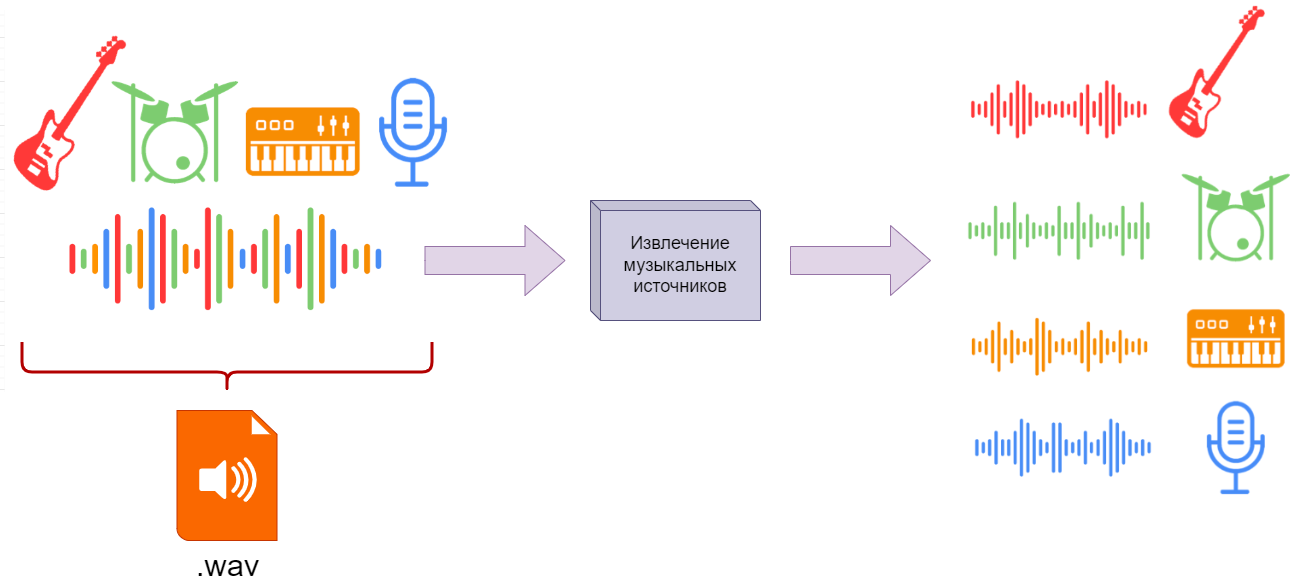
\includegraphics[width=1\textwidth]{figures/задача извлечения источников.png}
	\caption{Упрощенный процесс разделения источников из аудиозаписи. Авторский материал}
	\label{fig:sourcesep}
\end{figure}

\par Для разделения источников используются алгоритмы обработки сигналов, которые используют различные техники: 
спектральный анализ, анализ во временной и частотной областях, машинное обучение.
\par Итогом выполнения задачи декомпозиции смешанного аудиосигнала являются выходные данные в виде компонент, представляющих 
собой изолированные аудиодорожки исходного источника (например, партию гитары, барабанов или вокала). 
Такая аудиодорожка является единицей музыкального аудиопотока в задаче выделения источников. 
Когда происходит запись в студии звукозаписи, например, музыкального трека, то происходит запись отдельных музыкальных инструментов и вокала и образуется финальная композиция. 
И цель задачи извлечения сигналов, в том, чтобы воссоздать эти индивидуальные дорожки из смешанного сигнала-музыкальной дорожки.
\par Притом, такая задача подразумевает получение из одного аудиотрека (аудиопотока) несколько источников (то есть задача сложнее, 
чем из потока шума получить какой-то один источник – в статье~\cite{waveform_domain} приводится пример появления задачи – потребность услышать и вычленить 
из общего шума общественного места выделить голос и речь своего собеседника).

\par Таким образом, необходимо провести обзор и анализ методов разделения музыкальных источников, являющимися стандартами 
в наше время, определить возможные методы дообучения таких моделей, а также метрики, которыми можно оценить проведённое дообучение.

\subsection{Постановка задачи}
Задача извлечения источников из музыкального сигнала формулируется следующим образом~\cite{digital_signal}: <<Дан звуковой файл в формате .wav, 
содержащий запись нескольких музыкальных инструментов. Звуковой файл представляет собой оцифрованный аналоговый сигнал $x(t)$.
Необходимо найти аудиосигналы $\hat{s}_i$, удовлетворяющие следующим условиям>>.

\begin{equation*}
\begin{cases}
    x(t) = \displaystyle\sum_{i=1}^{N} s_i(t) + n(t), \\[8pt]
    \hat{s}_i(t) = \mathcal{F}(x(t), i) \approx s_i(t),
\end{cases}
\label{eq:task_system}
\end{equation*}

где
\begin{itemize}[label=$\bullet$, wide]
    \item $x(t)$ --- исходный смешанный аудиосигнал;
    \item $s_i(t)$ --- эталонный аудиосигнал $i$-го источника;
    \item $N$ --- количество источников в композиции;
    \item $n(t)$ --- шумовой компонент (помехи, внешние источники);
    \item $\mathcal{F}(x(t), i)$ --- оператор извлечения $i$-го источника, реализуемый нейросетевой архитектурой;
    \item $\hat{s}_i(t)$ --- аудиосигнал $i$-го источника, полученный оператором извлечения источников.
\end{itemize}


\subsection{Вклад кампании SiSEC MUS 2018 в задачу разделения источников}

\par В статье, посвящённой реализации нейронной сети Open-Unmix~\cite{openunmix} упоминается крупная международная
кампания SiSEC 2018 \cite{sigsep_camp, sigsep_camp2}, в рамках которой были стандартизированы подходы к оценке качества
разделения аудиоисточников. Среди основных задач данной кампании была задача извлечения из профессионально записаной музыки 
музыкальных инструментов по следующим общим категориям:
\begin{itemize}[label=$\bullet$, wide]
\item барабаны (drums),
\item бас (bass),
\item вокал (vocals),
\item другие музыкальные инструменты и звуки (other).
\end{itemize}

В рамках кампании SiSEC Mus 2018 сообществом исследователей был сформирован эталонный набор данных MUSDB18~\cite{MUSDB18}, 
содержащий 150 музыкальных композиций с разделенными аудио источниками в сумме составляющие 
10-часовой плейлист. 
Набор данных MUSDB18 всё ещё является самым большим бесплатным 
набором в открытом доступе и активно используется в задачах дообучения нейронных 
сетей, решающих задачу разделения источников ~\cite{waveform_domain} (при необходимости или скудности 
материалов этого набора данных исследователи прибегают к самостоятельному сбору специфичных наборов данных~\cite{MUSDB18_dop}).
Но чаще всего обучение больших базовых моделей, решающих задачу извлечения аудиоисточников, происходит именно на этом наборе.

\subsection{Способы представления звукового сигнала для задачи разделения источников}
Разные нейросетевые методы разделения музыкальных источников работают с разным представлением звукового сигнала. От того, какой
способ был выбран, зависит эффективность самого метода и его архитектура.
В современной литературе по цифровой обработке сигналов и машинному обучению выделяют три основных класса представлений \cite{stft_1977, hyb_spectr}:
\begin{itemize}[label=$\bullet$, wide]
	\item временное (waveform),
	\item частотное (spectral),
	\item частотно-временное (time-frequency).
\end{itemize}

\subsubsection{Временное представление}
Наиболее фундаментальным способом представления звука является дискретизированный временной сигнал $x[n]$, где $n = 0,1, \dots ,N-1$ 
--- номер отсчёта, $N$ --- общая длина сигнала. Значение $x[n]$ соответствует амплитуде звукового давления в момент времени $\frac{n}{f_s}$
где $f_s$ — частота дискретизации (обычно 44100 Гц или 48000 Гц для музыкального контента) \cite{spectral}.

С точки зрения физики временной сигнал отражает колебание давления воздуха, которые были зафиксированы микрофоном, 
записывающим аудиосигнал. Монофонический звуковой сигнал (моносигнал) представляет собой последовательность вещественных чисел $x[n]$, 
где каждый отсчёт отражает мгновенное значение амплитуды.
Для удобства обработки значения обычно нормализуются к диапазону $[-1,1]$ или сохраняются в стандартном цифровом формате PCM (импульсно-кодовая модуляция) 
с фиксированной разрядностью (например, 16 или 24 бита). Именно такой формат данных лежит в основе несжатых форматов (.wav, .aiff), а также 
служит промежуточным представлением при декодировании сжатых форматов (.mp3, .aac) перед их обработкой нейросетевыми алгоритмами.

В задачах разделения источников временное представление используется в архитектурах, работающих во временной области, таких как 
Conv-TasNet \cite{Conv-TasNet} и Demucs \cite{demucs, waveform_domain}, которые работают непосредственно с сырыми отсчётами, применяя одномерные свёртки 
для извлечения признаков.


\subsubsection{Частотно-временное представление}
Большинство современных методов разделения музыкальных источников работают во частотно-временной области,
применяя оконное преобразование Фурье (Short-Time Fourier Transform, STFT) 
для перевода исходного аудиосигнала в спектральное представление.
Характерным примером такой архитектуры является модель Open-Unmix \cite{openunmix}.

\par\textit{Оконное преобразование Фурье (ОПФ)} вычисляется путём разбиения дискретного сигнала $x[n]$ на перекрывающиеся сегменты (фреймы)
с помощью скользящего окна.
На каждом шаге локальный фрагмент сигнала умножается на оконную функцию $w[n]$, после чего к нему применяется дискретное преобразование
Фурье. Для обеспечения наложения соседних сегментов сигнала окно анализа последовательно смещается вдоль него с шагом $H$, 
который строго меньше длины окна $L$~\cite{stft_2008}:
\begin{equation*}
    X[m, k] = \sum_{n=0}^{L-1} x[n + mH] \cdot w[n] \cdot e^{-j 2\pi k n / L},
    \label{eq:stft}
\end{equation*}

где 
\begin{itemize}[label=$\bullet$, wide]
	\item $X[m, k] \in \mathbb{C}$ --- комплексное значение ОПФ для $m$-го временного сегмента и $k$-го частотного отсчёта;
	\item $L$ --- длина окна, количество отсчётов в одном сегменте (обычно это 2048 или 4096 отсчётов);
	\item $H$ --- шаг смещения окна, определяющий степень перекрытия соседних участков (обычно это $H = L/4$ или $H = L/2$);
	\item $w[n]$ --- оконная функция, применяемая к сегменту сигнала;
	\item $k = 0, 1, \dots, L/2$ --- индекс частотной компоненты  (соответствует физической частоте $f_k = k \cdot f_s / L$);
	\item $m = 0, 1, \dots, M-1$ --- индекс временного сегмента, где $M$ --- общее число фреймов;
	\item $j$ --- мнимая единица.
\end{itemize}

Физически оконное преобразование Фурье представляет собой переход от одномерного временного сигнала к двумерному 
частотно-временному представлению. 
Каждый комплексный коэффициент $X[m, k]$ характеризует амплитуду и фазу частотной компоненты $f_k$ в конкретный момент времени $t_m = mH/f_s$.

\par\textit{Спектрограмма} представляет собой двумерное представление сигнала, которое формируется на основе оконного 
преобразования Фурье (ОПФ) путём вычисления модуля или квадрата модуля его комплексных коэффициентов. 
В зависимости от цели анализа выделяют амплитудную и энергетическую спектрограммы:

\begin{equation*}
    S[m, k] = \lvert X[m, k] \rvert \quad \text{(амплитудная)},
    \label{eq:amp_spectrogram}
\end{equation*}

\begin{equation*}
    P[m, k] = \lvert X[m, k] \rvert^2 \quad \text{(энергетическая)},
    \label{eq:power_spectrogram}
\end{equation*}

На практике для сжатия широкого диапазона аудиосигнала часто применяется логарифмическое масштабирование:
\begin{equation*}
    S_{\text{log}}[m, k] = \log\left(1 + \lvert X[m, k] \rvert\right) \quad \text{(логарифмическая)}.
    \label{eq:log_spectrogram}
\end{equation*}

Визуально спектрограмма представляет собой двумерное изображение (тепловая карта), где по оси абсцисс 
откладывается время, по оси ординат --- частота, а яркость цвета на графике соответствует энергии 
соответствующей спектральной компоненты.
Для музыкальных сигналов такая визуализация позволяет наглядно выделить гармоническую структуру инструментов, 
проявляющуюся в виде горизонтальных полос на частотах, кратных основной частоте тона. 
Пример спектрограммы музыкального сигнала приведён на рисунке~\ref{fig:spectrogram}.

\begin{figure}[h!]
	\centering
	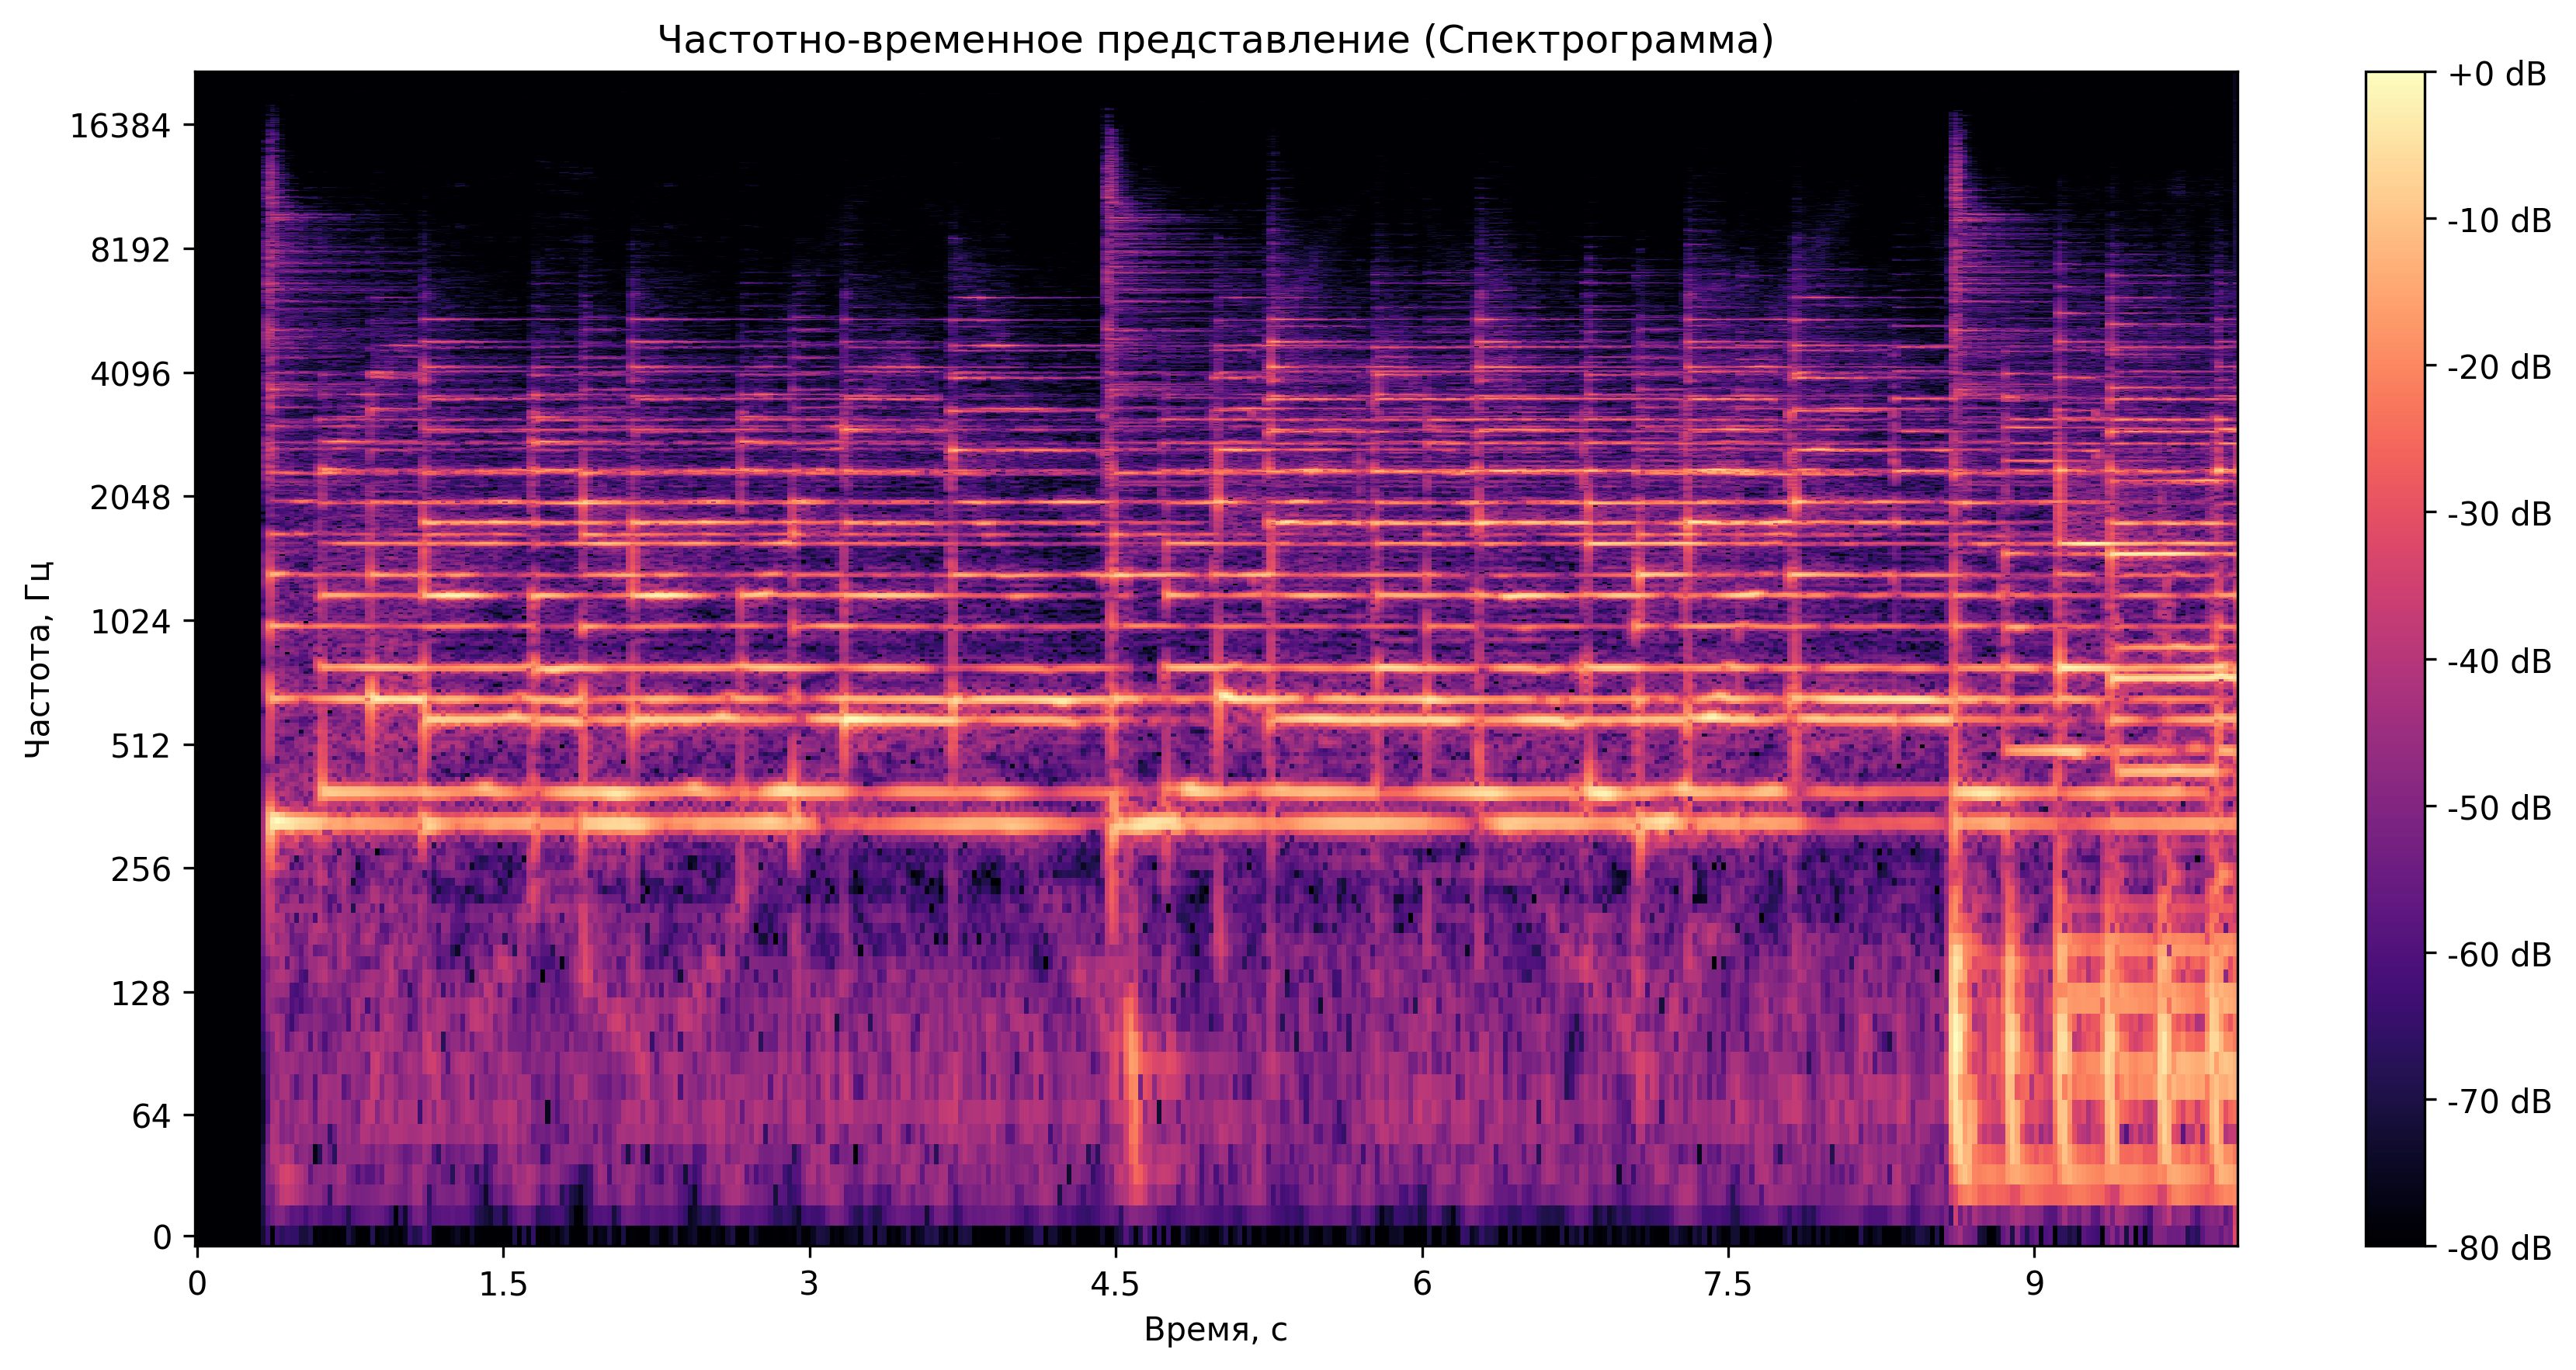
\includegraphics[width=1\textwidth]{figures/spectrogram.png}
	\caption{График спектрограммы музыкальной композиции. Авторский материал}
	\label{fig:spectrogram}
\end{figure}

В контексте задач разделения музыкальных источников спектрограмма служит в качестве основного входного представления 
для моделей, работающих в частотной области (например, Open-Unmix \cite{openunmix}).
В рамках такого подхода нейросетевая архитектура обучается предсказывать матрицы частотно-временных масок $M_c[m, k] \in [0, 1]$ 
для каждого источника $c$, которые затем применяются к исходному аудиосигналу для выделения отдельных компонент источников:
\begin{equation*}
    \hat{S}_c[m, k] = M_c[m, k] \cdot S_{\text{mix}}[m, k],
    \label{eq:masking}
\end{equation*}

\noindent где \begin{itemize}[label=$\bullet$, wide]
	\item $S_{mix}$ --- спектрограмма исходного музыкального файла;
	\item $\hat{S}_c[m, k]$ --- оценка спектрограммы $c$-го источника.
\end{itemize}

Для восстановления временного сигнала из спектрограммы применяется \textit{обратное ОПФ (iSTFT, inverse STFT)} (формула \ref{eq:istft}).

\begin{equation}
    \hat{x}[n] = \frac{1}{L} \sum_{m=0}^{M-1} \left( \frac{1}{2\pi} \sum_{k=0}^{L-1} \hat{X}[m, k] \cdot e^{j 2\pi k n / L} \right) \cdot w[n - mH],
    \label{eq:istft}
\end{equation}

\noindent где $\hat{X}[m, k]$ --- комплексная спектрограмма с применённой маской (сохраняется фаза исходной композиции или восстанавливается 
итеративными методами).

% -----------------  2. Обзор существующих аналогов, методов и технологий разработки аналогичных программ,
% -----------------  3. Объект и предмет исследования,
% -----------------  4. Постановка задачи,
% -----------------  5. Практическая и теоретическая значимость,
% -----------------  6. Используемые методы и технологии разработки ПО,
% -----------------  7. Краткие теоретические сведения.

\subsection{Обзор современных архитектур моделей разделения источников}

Современные архитектуры извлечения аудиоисточников можно условно разделить на два основных 
класса в зависимости от того, в какой области они обрабатывают аудиосигнал: во временной области (Demucs \cite{demucs}) 
или в частотной (Open-Unmix \cite{openunmix} и Spleeter \cite{Spleeter}). Далее рассмотрим эти основные виды архитектур и сравним их способы
 реализации и применение.

 \subsubsection{Архитектура модели Open‑Unmix} 

Архитектуры, работающие в частотной области (например, Open-Unmix~\cite{openunmix} и Spleeter), 
основаны на предварительном преобразовании входного временного аудиосигнала в спектрограмму с использованием оконного
преобразования Фурье. 
В таком представлении каждый элемент матрицы спектрограммы соответствует амплитуде (энергии) конкретной 
частотной компоненты в заданный момент времени. 

В процессе работы нейросетевая модель анализирует эту спектрограмму и предсказывает частотно-временные маски для 
каждого заданного источника. 
Далее полученная маска поэлементно умножается на спектрограмму исходного аудиомикса, после чего к 
результату применяется обратное оконное преобразование Фурье (iSTFT) для получения итоговой аудиодорожки источника. 

Детальная структура модели Open-Unmix, которая является на текущей момент эталонной реализацией спектрального подхода,
представлена в работе~\cite{openunmix}. Схема ее архитектуры приведена на рисунке ~\ref{fig:openunmix}. 
\begin{figure}[h!]
	\centering
	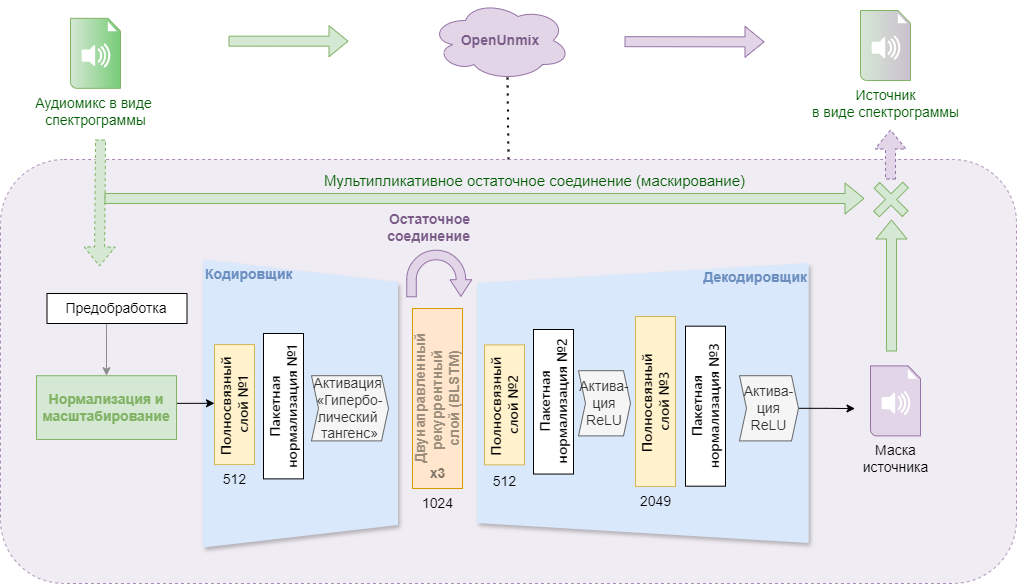
\includegraphics[width=1\textwidth]{figures/open unmix.png}
	\caption{Архитектура модели Open-Unmix. Авторский материал}
	\label{fig:openunmix}
\end{figure}

Общая идея модели Open-Unmix заключается в преобразовании исходного файла аудиомикса музыкальных 
инструментов в формате спектрограммы в набор спектрограмм отделенных музыкальных инструментов-источников из 
этого микса.

Модель Open-Unmix состоит из следующих компонентов:
\begin{enumerate}[label=\arabic*)]
\item Предобработка данных --- так как предобученная модель Open-Unmix обучалась на наборе данных MUSDB18~\cite{MUSDB18}, аудиозаписи которого 
подвергались AAC-сжатию, в результате которого диапазон спектрограмм обрезался до 16 кГц, в модели Open-Unmix на этапе предобработки
 входного сигнала выполняется <<обрезка>> спектрограммы по оси частот с исключением частотных ячеек, соответствующих более высоким частотам (больше 16 кГц).

\item Входная нормализация и масштабирование --- блок обучаемых аффинных параметров. Он выполняет нормализацию входных 
спектрограмм для улучшения качества работы модели с помощью поэлементного сдвига и масштабирования входных спектрограмм,
выравнивая распределение амплитуд по частотным каналам перед подачей на основные слои модели,
что ускоряет сходимость градиентного спуска.

\item Блок кодирования признаков (кодировщик) --- это совокупность механизмов и линейных слоёв внутри Open-Unmix, которая занимается сжатием 
входного аудиопотока в компактный набор признаков --- то есть выполняет проекцию высокоразмерного частотно-канального представления в компактное
 скрытое (латентное) пространство.
В отличие от классических кодировщиков, данный блок не стремится восстанавливать входной сигнал, а формирует признаки, оптимальные для 
последующего предсказания маски. Процесс кодирования включает:
    \begin{itemize}[label=$\bullet$, wide]
		\item Линейную проекцию (fc1, Fully Connected, первый полносвязный слой) --- линейный слой без смещения, формирующий точку максимального сжатия данных (<<узкое горлышко>>).
		Ограничение размерности на этом этапе принуждает модель отбрасывать избыточную спектральную информацию и шум, формируя наиболее плотное и информативное представление перед рекуррентной обработкой.
		\item Пакетную нормализацию (bn1, Batch Normalization layer, первый слой пакетной нормализации) --- это модуль, который выполняет стандартизацию выходных 
		значений полносвязного слоя, обеспечивая согласованность признаков перед их подачей на нелинейное преобразование $\tanh$.
		\item Функцию активации гиперболического тангенса (tanh) --- нелинейная функция активации, ограничивающая значения активации
		диапазоном $[-1, 1]$, что необходимо для устойчивой работы рекуррентных слоёв.
		Формула функции гиперболического тангенса имеет вид:
		\begin{equation}
			\label{eq:tanh}
			\tanh(x) = \frac{e^{x} - e^{-x}}{e^{x} + e^{-x}}
		\end{equation}
		где $x$ --- выход слоя нормализации.
	\end{itemize}
\item Центральный рекуррентный модуль --- представляет собой три последовательных реккурентных слоя 
двунаправленной долговременной краткосрочной памяти (Bidirectional Long Short-Term Memory, BLSTM). 
Его главная задача --- анализ временных зависимостей в сигнале.
Такая многослойная архитектура обеспечивает формирование признаков по принципу иерархии: начальные слои фиксируют кратковременные 
локальные особенности звучания (езкие всплески амплитуды, атаки звуков), а последующие слои последовательно 
объединяют эти данные, выявляя долгосрочные музыкальные закономерности (мелодические фрагменты, гармонические последовательности).

Для предотвращения исчезновения градиентов и сохранения спектральной информации при глубокой обработке на промежуточных этапах применяется 
механизм \textit{остаточного соединения (Skip Connection)}.
На схеме~\ref{fig:openunmix} он изображён фиолетовой стрелкой над блоком <<Двунаправленный рекуррентный слой>> и обозначает 
объединение входного тензора с результатом обработки блока BLSTM. Математически эта логика представлена в формуле \ref{eq:skipson}:
	\begin{equation}
		\label{eq:skipson}
		h = x + \mathcal{F}_{\mathrm{BLSTM}}(x),
	\end{equation}
где
	\begin{itemize}[label=$\bullet$, wide]
		\item $x$ --- входное представление размера 512,
		\item $\mathcal{F}_{\mathrm{BLSTM}}(\cdot)$ --- преобразование, выполняемое стеком BLSTM-слоёв.
	\end{itemize}

То есть данные из начала блока копируются в конец, минуя сложные вычисления. Это нужно, чтобы важная информация не потерялась при глубокой обработке.
Такой приём обеспечивает прямой градиентный поток и ускоряет сходимость оптимизатора.

\item Блок декодирования (декодировщик) --- отвечает за восстановление размерности тензора до исходных размеров 
для последующего формирования маски.
В отличие от классических декодеров, данный блок не обучается восстанавливать исходный сигнал, а предсказывает коэффициенты маски, 
которые при поэлементном умножении на входной спектр определяют целевой источник.

Архитектурно декодировщик зеркален кодировщику и включает:
    \begin{itemize}[label=$\bullet$, wide]
		\item Два полносвязных слоя (fc2 и fc3) --- слой fc2 проецирует объединённый вектор признаков из расширенного 
		пространства обратно в компактное представление, а слой fc3 расширяет его до исходного числа частотно-канальных коэффициентов, 
		формируя основу для последующего вычисления весовой маски.
        \item Два слоя пакетной нормализации (bn2 и bn3) --- стабилизируют распределение сигналов внутри пакета на промежуточных
		этапах восстановления.
        \item Функцию активации ReLU --- функция применяется после нормализации и на финальном выходе блока декодировщика.
		Формально функция определяется следующим образом:
			\begin{equation*}
				\label{eq:relu}
				\operatorname{ReLU}(x) = 
				\begin{cases} 
					0, & \text{если } x < 0, \\
					x, & \text{если } x \geq 0,
				\end{cases}
			\end{equation*}
	\end{itemize}
		Фунция ReLU заменяет все отрицательные значения нулями. 
		Это обеспечивает два важных свойства: во-первых, модель фокусируется только на значимых признаках, подавляя фоновый шум; 
		во-вторых, гарантируется неотрицательность итоговой маски, что соответствует физической природе амплитудного спектра, 
		потому что интенсивность частотных компонент не может принимать отрицательные значения.

\item Механизм мультипликативного маскирования (Multiplicative Skip-Connection) --- механизм финального выделения 
целевого источника, при котором исходный спектр аудиомикса поэлементно умножается на предсказанную 
маску только на выходе сети.
Такой подход предпочтительнее прямой генерации спектрограммы <<с нуля>>, так как позволяет переиспользовать фазовую информацию из 
исходного сигнала, избегая артефактов реконструкции. 
Модель Open-Unmix вычисляет широкополосную маску, значение которой в каждом частотно-временном элементе
 отражает долю энергии целевого источника в общем аудиомиксе. Процесс итогового разделения описывается формулой поэлементного умножения:
\begin{equation*}
    \hat{S} = X \odot \hat{M},
\end{equation*}
где 
\begin{itemize}[label=$\bullet$, wide]
	\item $X \in {R}^{T \times F}$ --- исходная спектрограмма аудиомикса (суммарное представление всех инструментов),
	\item $\hat{M} \in {R}^{T \times F}$ --- предсказанная нейросетью маска (выход модуля декодирования после функции активации
	 ReLU, обеспечивающей неотрицательность значений),
	\item $\hat{S}$ --- результирующая спектрограмма целевого аудиоисточника.
\end{itemize}
\end{enumerate}

Таким образом, архитектура Open-Unmix реализует сквозной конвейер частотно-временного разделения 
источников, в котором входная спектрограмма аудиомикса последовательно проходит через блок кодирования признаков, 
двунаправленную рекуррентную сеть для моделирования временных зависимостей и блок восстановления размерности, 
формирующий оценку маски для извлечения целевого сигнала. 
Финальное выделение изолированной дорожки осуществляется путём поэлементного умножения 
предсказанной маски на исходную спектрограмму, что обеспечивает восстановление целевого источника с сохранением фазовой информации и минимизацией 
артефактов, характерных для генеративных моделей.

Модель Open-Unmix  обладает рядом сильных сторон, однако имеет и специфические ограничения, которые важно учитывать при выборе базовой модели. 
Среди преимуществ можно отметить:
\begin{enumerate}[label=\arabic*)]
	\item Авторы модели Open-Unmix называют ей эталонной 
	реализацией~\cite{openunmix} для задач разделения источников. 
	Текст исходной программы, предобученные веса и документация находятся в открытом доступе, что обеспечивает полную воспроизводимость 
	результатов и упрощает интеграцию в исследовательские и прикладные проекты.
	\item Применение двунаправленной реккурентной LSTM-сети позволяет анализировать сигнал 
	как в прямом, так и в обратном направлении~\cite{BLSTM}.
	Это преимущество важно для разделения гармонических инструментов, где для корректного выделения аудиоисточника требуется понимание 
	всей музыкальной композиции вцелом.
	\item По сравнению с современными тяжёлыми гибридными 
	или генеративными архитектурами, Open-Unmix показывает конкурентноспособные значения метрик на эталонных наборах данных 
	при значительно меньших требованиях к вычислительным мощностям, что делает её удобной для экспериментов в условиях ограниченных ресурсов.
	\item Чёткое разделение на блоки кодирования, рекуррентной обработки и декодирования 
	позволяет адаптировать архитектуру под специфические задачи: замену слоёв BLSTM на трансформерные слои, добавление многозадачного
	обучения или расширение конвейера на новые классы источников.
\end{enumerate}

Но модель Open-Unmix также имеет следующие ограничения:
\begin{enumerate}[label=\arabic*)]
	\item Так как слои LSTM идет последовательно, это ограничивает возможности параллелизации при обучении и запуске модели. 
	Обработка длинных аудиопоследовательностей требует значительного времени и памяти, что затрудняет применение модели в 
	системах реального времени с жёсткими требованиями к низкой задержке.
	\item Подход на основе идеальных масок, которым оперирует модель Open-Unmix, предполагает, что источники в аудиомиксах независимы и их можно суммировать. 
	Когда инструменты занимают один частотный диапазон, модель вынуждена идти на компромисс при оценке весов. 
	Это приводит к взаимному <<перетеканию>> аудиосигналов: в выделенной дорожке одного инструмента остаются слышимые 
	фрагменты другого, так как сеть не может однозначно разделить общую энергию в этих частотах.
	\item Поскольку модель предсказывает только громкость частот (амплитуду), а фазу просто 
	копирует из исходного микса, это часто приводит к звуковым искажениям. Особенно это заметно 
	там, где волны разных инструментов в миксе конфликтовали друг с другом, вызывая на выходе 
	характерные <<фазовые артефакты>>, <<размытость звука>> или <<металлический>> призвук.
\end{enumerate}

Архитектура Open-Unmix представляет собой сбалансированное решение для задачи разделения музыкальных 
источников, сочетающее интерпретируемость, воспроизводимость и конкурентоспособное качество. 
Основные ограничения модели связаны с вычислительной сложностью рекуррентных блоков и допущениями, 
лежащими в основе подхода маскирования.

\subsubsection{Архитектура модели Spleeter}
Модель Spleeter — это система разделения музыкальных источников, разработанная компанией Deezer в 2019 году~\cite{Spleeter}. 
Модель основана на архитектуре U-Net~\cite{unet}, работающей в частотной области, и обучена на синтетически 
сгенерированном наборе данных из 25 тысяч композиций.
В отличие от рекуррентных подходов, модель Spleeter использует полностью сверточную архитектуру типа U-Net,
что обеспечивает высокую скорость обработки за счёт параллелизации вычислений.

Модель Spleeter стала одним из первых доступных промышленных решений для разделения звука. 
Она поддерживает выделение 2, 4 или 5 источников (вокал, ударные, бас, фортепиано и 
категория <<остальное>>), что обеспечило ей широкую популярность благодаря простоте использования.

Согласно официальной документации~\cite{SpleeterArch}, архитектура Spleeter состоит 
из следующих ключевых блоков:
\begin{enumerate}[label=\arabic*)]
	\item Подготовка входных данных. Исходный аудиосигнал $x(t)$ преобразуется в комплексную спектрограмму с помощью оконного 
	преобразования Фурье с размером окна 4096 и шагом сдвига 1024.
	\item Кодировщик. Его задача --- проанализировать входную спектрограмму и постепенно выделить из неё самые важные особенности звука. Для этого используется цепочка сверточных блоков. Каждый такой блок последовательно выполняет три действия:
	\begin{itemize}[label=$\bullet$, wide]
		\item применяет свёртку $3 \times 3$ с шагом 2, чтобы сжимать данные и уменьшать их размерность;
		\item проводит пакетную нормализацию;
		\item использует функцию активации ReLU.
	\end{itemize}
	\item Блок сжатия --- это центральная часть сети, где данные достигают минимальной размерности.
	Такое ограничение заставляет модель отбрасывать шум и второстепенные детали, фокусируясь исключительно на самых важных абстрактных 
    характеристиках музыкального сигнала.
	\item Декодировщик с остаточными связями. Этот блок постепенно восстанавливает 
	исходную размерность спектрограммы с помощью транспонированных сверток, объединяя сжатые признаки с деталями более ранних слоев
	для повышения точности восстановления.
	\item Генерация маски и восстановление сигнала. На выходе модель формирует весовую маску, которая поэлементно умножается на 
	исходную спектрограмму аудиомикса. Затем с помощью обратного оконного преобразования Фурье полученный 
    спектр преобразуется обратно в готовый аудиосигнал целевого источника.
\end{enumerate}

Модель Spleeter имеет следующие преимущества:
\begin{enumerate}[label=\arabic*)]
	\item Высокая скорость выполнения запроса. Благодаря полностью сверточной архитектуре без рекуррентных связей, 
	все вычисления могут быть распараллелены на графическом процессоре. Обработка трека происходит в 5–10 раз быстрее, чем в реальном 
	времени, что делает модель пригодной для потоковых сервисов.
	\item Эффективное сохранение деталей. Архитектура модели Spleeter, основанная на модели U-Net c 
	механизмом skip-connections озволяет восстанавливать высокочастотные компоненты, которые часто теряются в 
	архитектурах с сильным сжатием, обеспечивая «прозрачное» звучание.
	\item Устойчивость к переобучению. Использование пакетной нормализации и умеренной глубины сети 
	(по сравнению с Transformer-моделями) снижает риск переобучения на небольших наборах данных.
\end{enumerate}

Также существуют значимые ограничения в работе модели Spleeter:
\begin{enumerate}[label=\arabic*)]
	\item Частотные артефакты. Работа исключительно в магнитудной области с сохранением фазы из 
	аудиомикса приводит к артефактам в областях сильного спектрального перекрытия источников.
	\item Малая гибкость архитектуры. Фиксированная структура U-Net сложнее адаптируется под новые 
	классы источников или многозадачное обучение по сравнению с модульными подходами (Open-Unmix, Demucs).
	\item Модель Spleeter является устаревшей и не применяется в современных исследованиях в связи с тем, что больше не поддерживается разработчиками.
	У модели сохраняются зависимости от устаревших версий библиотек Python, что становится проблемой при исследовании.
\end{enumerate}

\subsubsection{Архитектура модели Demucs}

\par В статье~\cite{demucs} разработчики социальной сети Facebook описывают новый подход к методу извлечения источников. 
Demucs (Hybrid Transformer Demucs) на данный момент является одним из стандартов индустрии (SOTA --- state of the art) 
задачи извлечения источников.
\par Demucs~\cite{demucs} – это нейронная сеть глубокого обучения, которая была разработана для решения задачи 
выделения аудио-источников. В основе нейросети Demucs лежит свёрточная нейронная сеть UNet~\cite{unet}, 
которая используется для семантической сегментации изображений. То есть Demucs использует подход 
сети Unet обработки изображений и применяет для обработки волн аудиосигнала по спектрограммам~\cite{demucs}.
\par В статье музыкальная композиция сравнивается с коктейльной вечеринкой, где каждый голос, 
фоновая мелодия и шум – каждый этот элемент является стемом, и тогда задача выделения голоса собеседника,
 с которым ведется диалог на вечеринке, является как раз задачей разраделения источников. 
 Но задача выделения источников из музыкальной композиции отличается от задачи выделения голоса собеседника 
 на в первую очередь тем, что в ней интересует в этой задаче выделение не 
 какого-то одного приоритетного источника звука из несвязанного фонового шума, а целый набор тонов и 
 тембров в согласованном потоке.
\par Разработчики модели Demucs основываются на архитектуре Conv-Tasnet и адаптируют ее под извлечение 
источников, т.к. изначально модель Conv-Tasnet предназначалась для извлечения речи из аудиопотока \cite{Conv-TasNet}.
% \par https://docs.google.com/spreadsheets/d/1lIi9ijNv80Ri0ZBvqT3l41x0mEp1WcwK_03Jp97BIdU/edit?gid=0#gid=0 

Модель Demucs (в актуальных версиях v3/v4~\cite{demucs}) представляет собой гибридную архитектуру, 
объединяющую свёрточные нейронные сети, трансформерные блоки и параллельную обработку аудиосигнала 
как во временной области (waveform domain), так и в частотной (спектрограмма на основе ОПФ). 
В отличие от традиционных методов, которые предсказывают только амплитудные маски, Demucs одновременно 
анализирует амплитуду и фазу сигнала. Это позволяет точнее восстанавливать временную структуру звука и 
избегать характерных искажений, возникающих при простом умножении спектра на маску.
Архитектура модели Demucs представлена на рисунке \ref{fig:demucs}.

\begin{figure}[h!]
	\centering
	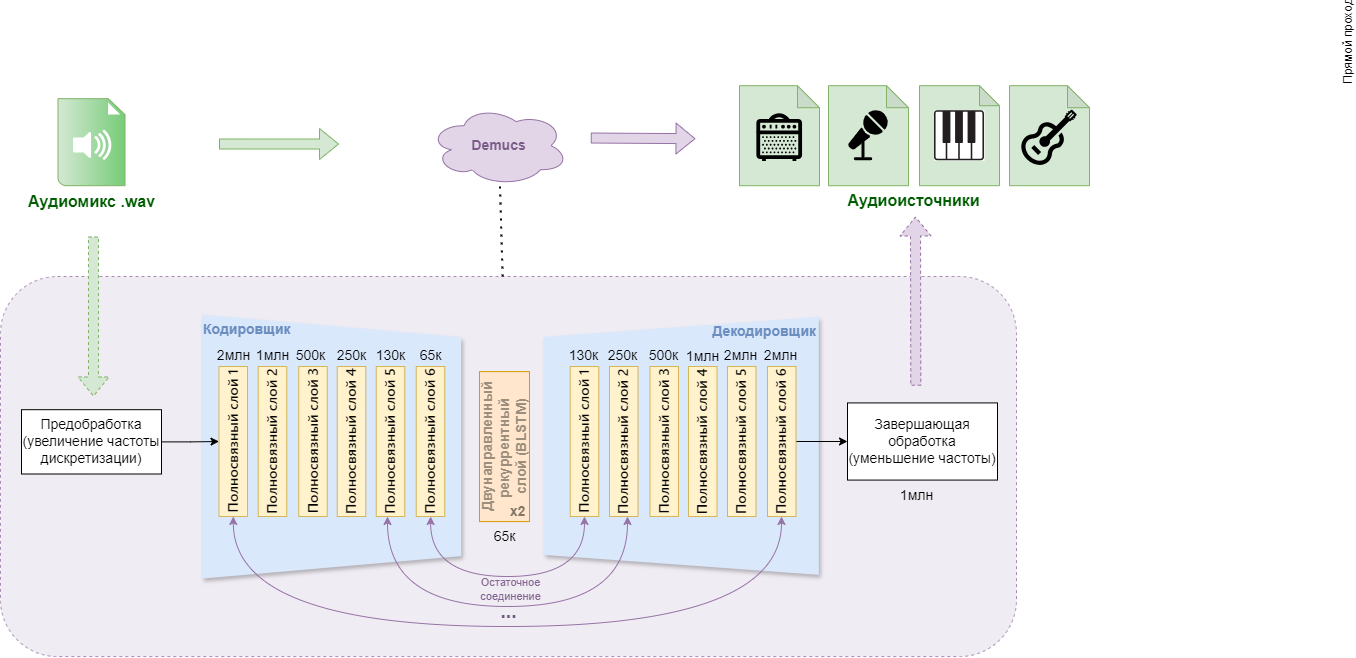
\includegraphics[width=1\textwidth]{figures/demucs схема.png}
	\caption{Схема архитектуры модели Demucs. Авторский материал}
	\label{fig:demucs}
\end{figure}


Модель Demucs состоит из следующих основных компонент:
\begin{enumerate}[label=\arabic*)]
	\item Гибридный кодировщик. Исходный аудиосигнал преобразуется в сжатое представление с помощью одномерных сверточных 
	слоев. Особенность модели HT Demucs в том, что она анализирует сигнал одновременно и как звуковую волну, и как спектрограмму (в этом и заключается <<гибридность>> модели).
	Это позволяет объединить высокую точность во времени с пониманием частотной структуры моделью.
	\item Блок разделения. На этом этапе используются слои трансформера. В отличие от рекуррентных сетей (применяемых, 
	например, в Open-Unmix), механизм внимания позволяет модели анализировать всю композицию целиком, а не только короткие 
	фрагменты. Это критически важно для качественного разделения инструментов с долгим и сложным звучанием.
	\item Гибридный декодировщик. Здесь сжатые данные преобразуются обратно в звуковой сигнал с помощью обратных сверточных слоев. 
	Декодировщик также работает в двух режимах: он восстанавливает и временную волну (с помощью одномерных сверточных слоёв), 
	и частотный спектр (с помощью двумерных свёрточных слоёв), а затем суммирует эти результаты для получения итогового звука.
	\item Расчёт гибридной функции потерь. При обучении модель оценивает неточности одновременно и во временной, и в частотной области. 
	Благодаря этому итоговый результат получается естественным на слух и корректным по своему спектральному составу.
\end{enumerate}

Главное преимущество модели Demucs как модели, работающей непосредственно с исходной звуковой волной и обрабатывающей аудиосигнал
в виде последовательности амплитудных значений (волн), заключается в сохранении полной информации о сигнале, включая его фазовые характеристики. 
Это критически важно для четкого и естественного воспроизведения резких звуков, таких как щипок струны гитары или удар по барабану, 
которые часто <<размываются>> при работе исключительно со спектрограммами.

Также к преимуществам модели Demucs относятся:
\begin{enumerate}[label=\arabic*)]
	\item На эталонных наборах данных (например, MUSDB18) модель Demucs демонстрирует показывают результаты 
	лучше, чем рекуррентные архитектуры эталонных наборах данных (например, Open-Unmix), особенно по метрикам общего 
	качества сигнала (SDR) и отсутствия посторонних шумов (SAR).
	\item Благодаря механизму внимания модель анализирует не просто короткие отрезки звука, а целые музыкальные фразы. 
	Это помогает ей гораздо эффективнее разделять инструменты со схожим тембром, опираясь на общую структуру композиции.
	\item Поскольку модель оптимизируется одновременно и по временным, и по частотным характеристикам, итоговый результат 
	получается естественным на слух и при этом математически точным по своему спектру.
\end{enumerate}

Однако у модели Demucs также есть свои ограничения, которые создают препятствия при её использовании 
в исследовательских работах:
\begin{enumerate}[label=\arabic*)]
	\item Из-за особенностей работы трансформера затраты ресурсов растут очень быстро при увеличении длины аудио. 
	Это требует значительно больше видеопамяти и времени на обработку по сравнению с более легкими моделями.
    \item Модель Demucs v4 содержит сотни миллионов параметров. Без специальных методов сжатия такую архитектуру 
	практически невозможно запустить на устройствах с ограниченными ресурсами.
	\item В случаях, если два инструмента играют одновременно и сильно перекрываются по частотам, модель иногда 
	начинает <<додумывать>> звук, создавая фантомные шумы или искажения там, где их быть не должно.
\end{enumerate}


\subsection{Анализ методов дообучения предобученных моделей разделения источников}

Существуют задачи, в рамках которых средств существующих предобученных нейронных сетей недостаточно и возникает потребность
провести над выбранной нейронной сетью ряд действий, позволяющих <<научить>> её тому контексту, которому она не была
<<обучена>> ранее, в процессе основного обучения, и которого не хватает для решения специфичной исследовательской задачи. 
При этом чаще всего такое обучение требуется провести без утраты тех <<знаний>>, которым была обучена модель первоначально,
 так как повторное переобучение модели с нуля --- дорогостоящий процесс, требующий больших вычислительных мощностей, больших 
 наборов данных, настройки всех параметров и т.д.

В таких случаях современные исследователи прибегают к подходу дообучения модели, в рамках которого модель не требуется переобучать
заново, но необходимо провести её <<тонкую настройку>> (fine-Tuning)~\cite{finetune, goodfellow} --- то есть на уровне механики модели провести некоторые действия, чтобы
научить нейронную сеть новым концептам с максимальным сохранением предыдущего накопленного опыта.

В случае задачи разделения источников в аудиосигнале обучение предобученной архитектуры модели с открытым исходным кодом 
на целевом наборе данных позволяет адаптировать модель к специфическим классам источников, о которых  модель не <<знала>>
 и которые не умела извлекать до этого, без необходимости обучения «с нуля».

Метод <<тонкой настройки>> в настоящее время широко применяется на различных предобученных нейросетевых моделях, включая модели извлечения аудиоисточники.
В зависимости от вычислительных ограничений и объёма данных для решения задачи дообучения применяется одна из трех основных стратегий: 
полная тонкая настройка, частичная настройка выходного блока и адаптация низкого ранга~\cite{finetune2}.

% https://temofeev.ru/info/articles/kak-doobuchat-ogromnye-modeli-s-maksimalnym-kachestvom-i-minimalnymi-zatratami-lora/
% https://dzen.ru/a/Z6sLY3hq8hZHohH-
% https://truetech.dev/ru/ai-development/services/llm/llm-lora-fine-tuning.html

\subsubsection{Полное дообучение}

Полное дообучение представляет собой стратегию обновления всех весов предобученной модели на новом,
 целевом наборе данных (например, полное дообучение применялось в работе \cite{finetune_piano_guitar}). 
 Все параметры предобученной модели размораживаются, и оптимизатор обновляет веса всех слоёв на
 новом наборе данных. 
 Обучение проводится с пониженным коэффициентом обучения (learning rate), 
 чтобы не разрушить уже усвоенные при первичном обучении спектрально-временных представлений, 
 но позволить сети адаптироваться к новому распределению данных.

В контексте задач разделения музыкальных источников данный подход подразумевает дообучение всей 
архитектуры на целевом наборе данных, содержащем изолированные партии инструментов, отсутствующие в 
исходном распределении модели. 
На предварительном этапе конфигурация выходного слоя адаптируется под новое количество источников, после
 чего оптимизатор обновляет веса всех слоёв сети, обеспечивая полную адаптацию внутренних спектрально-временных
представлений к специфике целевых классов.

Основное преимущество данного подхода — максимальная гибкость адаптации модели к специфике задачи,
 в том числе к особенностям частотного диапазона и перекрытию гармоник между инструментами. 
Также к преимуществам можно отнести:
\begin{enumerate}[label=\arabic*)]
  \item Простота реализации, метод не требует модификации архитектуры, чаще всего достаточно внести небольшое количество 
  изменений.
  \item При достаточном объёме наборов данных данный метод демонстрирует хорошее качество разделения источников \cite{demucs, finetune-2024}.
\end{enumerate}

Несмотря на высокую эффективность, стратегия сопряжена с существенными вычислительными и методическими ограничениями. 
Полное обновление весов требует значительного объёма видеопамяти для хранения градиентов и состояний оптимизатора,
 что часто делает процесс недоступным в средах с ограниченным аппаратным бюджетом \cite{LoRA}.
Кроме того, метод критически зависит от объёма и качества целевой выборки: при недостатке данных высок риск 
переобучения на специфичные акустические условия записей, а некорректно подобранные гиперпараметры могут привести к катастрофическому 
забыванию базовых признаков. 
В связи с этим полное дообучение целесообразно применять при наличии достаточных вычислительных ресурсов и сбалансированного 
набора данных.


\subsubsection{Методы «параметрического» дообучения (адаптация части параметров)}

Существует класс методов, которые отталкиваясь от концепции метода полного дообучения, дообучают не полностью
всю модель, а только часть её весов:  замораживают основную массу весов предобученной модели и обучают лишь 
малую добавочную часть параметров (обычно < $5\%$ от общего числа). Такие методы называют <<частичным дообучением>>
или <<параметрически эффективная адаптация>> \cite{peft}.

Суть метода заключается в том, что все слои кодировщика и рекуррентного/сверточного блока, размораживается 
только выходной слой (декодировщик или классификационная <<голова>>, выходной слой)~\cite{goodfellow}. 
Модель использует предобученные признаки общего звукового представления, 
а перестраивается только механизм соответствия признаков в целевые маски источников ~\cite{goodfellow}.

Использование методов параметрически эффективной адаптации (PEFT) имеет несколько явных преимуществ перед полным переобучением модели:
\begin{enumerate}[label=\arabic*)]
\item Поскольку в процессе обучения обновляется лишь небольшая часть весов сети, процесс проходит значительно быстрее и 
требует гораздо меньше видеопамяти~\cite{goodfellow}.
\item Заморозка основных слоев сети защищает модель от <<катастрофического забывания>>: она не утрачивает общие акустические 
закономерности, усвоенные при первоначальном обучении на больших массивах данных~\cite{SpeechSep, goodfellow}.
\item Низкие затраты на обучение позволяют исследователю быстро проверять различные гипотезы, менять состав обучающей 
выборки и подбирать гиперпараметры, не ожидая результата несколько дней~\cite{goodfellow}.
\end{enumerate}

Однако у такого подхода есть и свои ограничения, которые важно учитывать:
\begin{enumerate}[label=\arabic*)]
\item Если целевой инструмент звучит принципиально иначе, чем то, на чем училась базовая модель, замороженные слои 
не смогут полноценно подстроиться под новые спектральные особенности этого инструмента. 
В результате качество разделения достигнет предела своей эффективности.~\cite{SpeechSep}.
\item Модель, эффективно дообученная на чистых студийных записях, часто теряет качество при работе с более сложными 
материалами. Например, при обработке концертных записей или аудиоnтреков с артефактами сжатия ей не хватает внутренней гибкости 
для полной перестройки своих представлений, в отличие от модели, обученной с нуля непосредственно на таких данных ~\cite{SpeechSep}.
\end{enumerate}


\subsubsection{Адаптация низкого ранга (LoRA, Low Rank Adaptaion)}

Метод LoRA (Low Rank Adaptaion --- дословно переводится как <<адаптация на основе низкого ранка>>) был разработан для 
больших языковых генеративных моделей~\cite{LoRA}, но нашёл применение в большом пласте работ по дообучению моделей 
в машинном обучении, например, активно используется при дообучении генеративных моделей \cite{LoRA-sd}. 
Этот метод --- наиболее распространённая реализация парадигмы параметрически эффективного дообучения.

Основное отличие LoRA от методов полного дообучения и частичного дообучения заключается в том, что здесь адаптируется некоторое
количество параметров, результатом метода LoRA являются те веса, которые были преобразованы.
Низкоранговые методы дообучения основаны на идее замены части весов матриц на низкоранговые приращения, которые обучаемы,
 а исходные веса при этом остаются неизменными. Подход LoRA схематично представлен на рисунке ~\ref{fig:lora}.

Суть подхода LoRA представлена в названии метода: исследователи при создании этого метода проверяли гипотезу, которая заключалась 
в том, что внутренняя размерность (ранг) матрицы весов $\Delta W = W_{fine\_tuning} - W_0$ (где $W_{fine\_tuning}$ --- веса модели 
после дообучения, $W_0$ --- веса исходной модели) в больших моделях обладает низким рангом, несмотря на то, что 
исходная матрица весов $W_0$ имеет полный ранг. Это явление объясняется избыточной параметризацией современных 
нейросетей~\cite{LoRA23}: число обучаемых параметров значительно превышает минимально необходимое для решения задачи, что позволяет
 оптимизатору концентрировать полезные градиенты в низкоранговом подпространстве без потери обобщающей способности 
 (то есть <<предыдущих знаний>>).

\begin{figure}[h!]
	\centering
	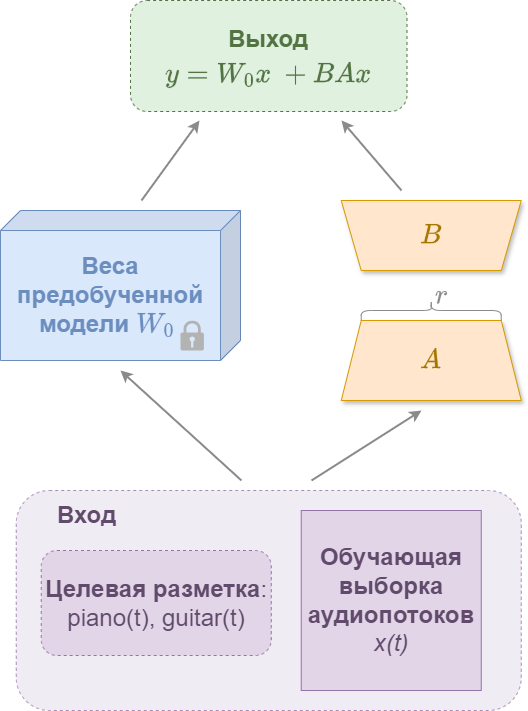
\includegraphics[width=0.5\textwidth]{figures/lora.png}
	\caption{Схема обучения модели подходом LoRA. Авторский материал}
	\label{fig:lora}
\end{figure}

Такое предположение позволяет декомпозировать изменение весов в виде произведения двух матриц более низкого ранга, чем матрица весов
 (а не оптимизировать саму матрицу весов изменяемого слоя):
\begin{equation*}
    \Delta W = BA,
\end{equation*}

где 
\begin{itemize}[label=$\bullet$, wide]
	\item $A \in R^{r \times k}$ --- матрица размерности ${r \times k}$,
	\item $B \in R^{d \times r}$ --- матрица размерности ${d \times r}$,
	\item $r \ll \min(d, k)$ --- ранг матрицы $W$, должен быть как можно меньше.
\end{itemize}

В процессе дообучения методом LoRA корректируются только матрицы $A$ и $B$ (считаются их градиенты и обновляются), 
что позволяет существенно снизить объём обучаемых параметров и требования к памяти GPU. Модель обучается лишь в низкоранговом 
подпространстве, которое описывается этими низкоранговыми матрицами, причём веса модели 
$W_0$ замораживаются и не преобразуются. Для получения итогового результата матрицы складываются:

\begin{equation}
    y = W_0x + \Delta Wx = W_0x + BAx,
\end{equation}

где 
\begin{itemize}[label=$\bullet$, wide]
	\item $A$ инициализируется Гауссовским распределением $A = N(0, \sigma^2)$,
	\item $B$ инициализируется 0,
	\item $W_0$ --- исходная матрица обучаемой модели.
\end{itemize}

Таким образом, LoRA заменяет полное обновление весов на обучение только компактных адаптеров, что сокращает 
количество обновляемых параметров на 70–91\%~\cite{LoRA}, снижает потребление видеопамяти и минимизирует риск катастрофического 
забывания исходных знаний модели, который часто сопутствует методам полного дообучения. В задаче выделения аудио источников, 
метод LoRA может применяться к отдельным слоям или компонентам модели (например, слоям свёртки или частотно‑временным модулям), 
что позволяет выполнять адаптацию параметров без изменения архитектуры исходной сети.

Среди преимуществ метода разработчики LoRA приводят следующие~\cite{LoRA}:
\begin{enumerate}[label=\arabic*)]
	\item Адаптеры LoRA небольшого размера, в связи с чем требования к размеру ресурсов для их расположения достаточно снижены.
	\item Поскольку градиенты вычисляются только для небольшого числа новых параметров, нагрузка на видеокарту резко снижается. 
	Это позволяет дообучать крупные нейронные сети даже на бесплатных тарифах облачных сервисов (например, Google Colab).
	\item Веса адаптеров A и B сохраняются отдельно от основной модели. Их можно быстро загружать, заменять или комбинировать без внесения изменений в архитектуру исходной модели.
	В рамках задачи извлечения источников, это позволяет поддерживать библиотеку адаптеров для различных инструментов 
	и комбинировать их при запуске модели.
	\item Поскольку основные веса модели $W_0$ остаются замороженными, она не теряет общие закономерности, которые усвоила при первоначальном 
	обучении на больших массивах данных.
\end{enumerate}

Однако у метода есть и свои ограничения, которые важно учитывать при выборе стратегии дообучения:
\begin{enumerate}[label=\arabic*)]
	\item Необходимость подбора ранга r. Значение ранга r является гиперпараметром, требующим эмпирической настройки.
	Если выбрать слишком маленькое значение, модель не сможет достаточно подстроиться под новую задачу. 
	Если слишком большое --- пропадёт главное преимущество метода, заключающеся в виде экономии ресурсов, и он станет почти сопоставим с полным дообучением.
	\item Метод LoRA исходит из того, что для адаптации к новой задаче нужны лишь небольшие корректировки весов. 
	Если новые данные сильно отличаются от тех, на которых модель училась изначально (например, переход от чистых студийных треков к 
	зашумлённым концертным записям), этих корректировок может не хватить. 
	В таких ситуациях полное переобучение часто показывает лучшие результаты и быть более эффективным решением.
\end{enumerate}


\subsection{Метрики оценки качества (SDR, SIR, SAR)}

В основных исследованиях, направленных на изучение дообучения моделей разделения источников, полученные результаты 
оцениваются при помощи метрик, которые являются стандартами в части оценки ~\cite{metrics}.

% demucs:   SDR, SIR, SAR, 
% spleeter: SDR, SIR, SAR, ISR
% unmix:    SDR, 

% итого:
% SDR (Signal to Distortion Ratio)
% SIR (source to interference ratio)
% SAR (sources to artifacts ratio)
% ISR / SI-SDR (source Image to Spatial distortion Ratio)
% Human evaluations

Чтобы объективно сравнить, насколько хорошо модели разделяют звук, недостаточно субъективной оценки.
В этой области приняты математические стандарты, которые сравнивают предсказанный моделью сигнал аудиоисточника $\hat{s}_k$ 
с идеальным эталоном $s_k$~\cite{metrics}. 

Главная идея этих метрик заключается в том, чтобы разделить общую ошибку на независимые составляющие. 
Оценивается не просто общая разница в сигналах, а определяется, что именно пошло не так: остались ли в выделенной дорожке источника
звуки других инструментов (интерференция) или добавил ли алгоритм свои посторонние шумы и искажения (артефакты). 
Такой подход позволяет независимо оценить два ключевых аспекта: насколько чисто и естественно выделен целевой инструмент и насколько эффективно 
подавлены все остальные.

В данной работе применяются классические метрики семейства BSS Eval (Blind Source Separation Evaluation)~\cite{metrics}, 
а также их современная модификация SI-SDR. Выбор конкретных показателей для каждой модели опирается на стандарты, 
заданные в оригинальных статьях этих архитектур:
\begin{itemize}
    \item для Open-Unmix~\cite{openunmix} ключевым показателем традиционно выступает общий SDR;
    \item для Demucs~\cite{demucs} и Spleeter~\cite{Spleeter} принято оценивать полный набор характеристик: SDR, SIR и SAR.
\end{itemize}
Следование этим устоявшимся стандартам оценки гарантирует, что оценка будет методологически корректна, 
а полученные результаты можно будет честно сопоставить с эталонными показателями.

\subsubsection{Декомпозиция сигнала по методу BSS Eval}
Согласно методологии оценки сигнала BSS Eval~\cite{metrics}, восстановленный сигнал аудиоисточника $\hat{s}$ может быть представлен в виде суммы
независимых друг от друга составляющих в соответствии с формулов~\ref{eq:signal_sum}:
\begin{equation}
	\label{eq:signal_sum}
    \hat{s} = s_{\mathrm{target}} + e_{\mathrm{interf}} + e_{\mathrm{noise}} + e_{\mathrm{artif}},
\end{equation}
где
\begin{itemize}[label=$\bullet$, wide]
	\item $\hat{s}$ --- сигнал, полученный алгоритмом извлечения аудиоисточников;
	\item $s$ --- эталонный сигнал исходного аудиоисточника;
	\item $s_{\mathrm{target}}$ --- компонента, представляющая собой проекцию сигнала $\hat{s}$ на пространство истинного сигнала $s$;
	\item $e_{\mathrm{interf}}$ --- компонента интерференции (другие посторонние источники, не относящиеся к источнику $s$);
	\item $e_{\mathrm{noise}}$ --- компонента шума (фоновый шум, шум оборудования, не связанный с источниками);
	\item $e_{\mathrm{artif}}$ --- компонента артефактов (искажения, внесённые алгоритмом).
\end{itemize}

Поскольку в стандартных музыкальных датасетах (например, MUSDB18) нет отдельной дорожки с фоновым шумом, компонентой $e_{\mathrm{noise}}$ 
пренебрегают и её объединяют с артефактами $e_{\mathrm{artif}}$. 
Оба этих слагаемых представляют собой искажения, не относящиеся ни к целевому инструменту, ни к интерференции. 
В популярной библиотеке \texttt{mir\_eval} шум также не выделяется отдельно, если для него не задан строгий эталон. 
Таким образом, формула декомпозиции сигнала упрощается до следующей:
\begin{equation*}
    \hat{s} \approx s_{\mathrm{target}} + e_{\mathrm{interf}} + e_{\mathrm{artif}}.
\end{equation*}

На основе этого разложения вычисляются три основные метрики (в децибелах, дБ), каждая из которых отвечает за свой аспект качества:
\begin{itemize}[label=$\bullet$, wide]
    \item SDR показывает общее качество разделения, учитывая все типы ошибок сразу.
    \item SIR демонстрирует, насколько эффективно модель подавила посторонние инструменты.
    \item SAR оценивает, насколько чистым получился звук без посторонних шумов, внесенных самим алгоритмом.
\end{itemize}

Метрика \textit{SDR (Signal-to-Distortion Ratio, отношение сигнала к искажению)} оценивает
общее отношение энергии оцениваемого сигнала $s_{\mathrm{target}}$ к суммарной энергии всех ошибок, возникающих в процессе разделения.
(например, наличие артефактов и наложения на источник других аудиоисточников).

Формула~\ref{eq:SDR} описывает математическое определение метрики SDR:
\begin{equation}
	\label{eq:SDR}
    \mathrm{SDR} = 10 \log_{10} \left( \frac{\lVert s_{\mathrm{target}} \rVert_2}{\lVert e_{\mathrm{interf}} + e_{\mathrm{artif}} \rVert_2} \right),
\end{equation}

\noindent где $\lVert \cdot \rVert_2$ --- квадрат Евклидовой нормы вектора дискретного сигнала.

Чем выше значение метрики SDR, тем лучше качество полученного источника. 
Значение 0 дБ означаетчто энергия полезного сигнала равна энергии ошибок. Положительные значения указывают на 
преобладание полезного сигнала. Увеличение значения метрики SDR на 10 дБ соответствует десятикратному 
улучшению отношения сигнал к ошибке. В исследованиях по разделению аудиоисточников~\cite{demucs, Spleeter, openunmix} метрика SDR служит 
критерием при сравнении качества моделей.

\par Метрика \textit{SIR (Signal-to-Interference Ratio, отношение сигнала к интерференции)} измеряет способность модели 
подавлять другие источники в исходном аудиомиксе.
Эта метрика игнорирует артефакты и шум, фокусируясь исключительно на <<чистоте>> разделения: насколько хорошо алгоритм 
отделил, например, вокал от аккомпанемента.
Формула~\ref{eq:SIR} описывает математическое определение метрики~SIR:

\begin{equation}
	\label{eq:SIR}
    \mathrm{SIR} = 10 \log_{10} \left( \frac{\lVert s_{\mathrm{target}} \rVert_2}{\lVert e_{\mathrm{interf}} \rVert_2} \right).
\end{equation}

Высокие значения SIR (например, >10–15 дБ) означают, что в выделенной дорожке практически не слышно других инструментов
и это свидетельствуют о качественном разделении источников.
Однако высокий SIR не гарантирует высокого субъективного качества: сигнал может быть <<чистым>> от других инструментов, 
но при этом содержать сильные артефакты обработки (эффект <<под водой>>, фазовые искажения), которые метрика SIR не учитывает, но учитывают другие метрики.

\par Метрика \textit{SAR (Signal-to-Artifacts Ratio, отношение сигнала к артефактам)} оценивает естественность звучания выделенного источника, абстрагируясь от наличия других инструментов.
Метрика чувствительна именно тем к искажениям, которые вносит метод разделения: эхо, фазовые сдвиги, <<музыкальный шум>>.
Формула~\ref{eq:SAR} описывает математическое определение метрики~SAR:

\begin{equation}
	\label{eq:SAR}
    \mathrm{SAR} = 10 \log_{10} \left( \frac{\lVert s_{\mathrm{target}} + e_{\mathrm{interf}} \rVert_2}{\lVert e_{\mathrm{artif}} \rVert_2} \right).
\end{equation}

Низкие значения метрики SAR часто указывают на наличие слышимых артефактов, даже если значение общей метрики SDR высокое.
Для задач, где важно естественное звучание (например, реставрация или улучшение качества), SAR является критически важным показателем.
Для моделей, работающих со спектрограммами (Open-Unmix~\cite{openunmix}, Spleeter~\cite{Spleeter}), низкое значение SAR часто указывает на ошибки, 
возникающие при некорректном применении частотной маски.

\subsubsection{Метрика SI-SDR, масштабно-инвариантное отношение сигнала к искажению}
Классические метрики чувствительны к громкости сигнала: например, если модель выдаёт правильный по форме, но более тихий сигнал, 
значение метрики SDR будет занижено.

Метрика \textit{SI-SDR (Scale-Invariant SDR, масштабно-инвариантное отношение сигнала к искажению)} устраняет эту зависимость: она 
предварительно нормализует предсказанный сигнал по громкости относительно эталона. 
Таким образом, метрика оценивает только сходство формы сигнала, игнорируя разницу в общей амплитуде.

Пусть $s$ — эталонный сигнал, $\hat{s}$ — оцениваемый предсказанный сигнал. Определим проекцию оценки $\hat{s}$ на направление эталонного сигнала $s$:

% Проекция оценки на направление эталонного сигнала
\begin{equation*}
    \alpha = \frac{\langle \hat{s}, s \rangle}{\lVert s \rVert_2}, \quad s_{\mathrm{proj}} = \alpha s,
\end{equation*}

\noindent где
\begin{itemize}[label=$\bullet$, wide]
	\item $\langle \cdot, \cdot \rangle$ --- скалярное произведение,
	\item $\alpha$ --- оптимальный коэффициент масштабирования.
\end{itemize}

Тогда итоговая метрика вычисляется следующим образом:

\begin{equation*}
    \mathrm{SI\text{-}SDR} = 10 \log_{10} \left( \frac{\lVert s_{\mathrm{proj}} \rVert_2}{\lVert s_{\mathrm{proj}} - \hat{s} \rVert_2} \right).
\end{equation*}

Эта метрика особенно полезна для моделей временной области (например, Demucs или Conv-TasNet~\cite{demucs}), 
где выходная амплитуда может варьироваться в процессе обучения.
Кроме того, метрика SI-SDR является дифференцируемой функцией, что позволяет использовать её непосредственно в качестве 
функции потерь при обучении нейронных сетей.

\subsection{Выводы}
В данной главе были рассмотрены теоретические основы задачи разделения музыкальных источников. 
Бали рассмотрены основные способы представления аудиосигнала (временной и частотный), а также математическое определение
оконного преобразования Фурье, лежащее в основе формирования спектрограмм.
Также были рассмотрены принципы работы ключевых современных нейросетевых архитектур, выявлены их особенности и ограничения. Был рассмотрен
математический аппарат для объективной оценки их качества таких архитектур.
Изучены стратегии дообучения предобученных нейросетевых моделей, сравнены подходы полного дообучения и параметрически эффективной настройки.

Проведённый в главе анализ позволил сделать выбор моделей и стратегий дообучения для дальнейшего исследования:
\begin{enumerate}[label=\arabic*)]
    \item В качестве базовых моделей выбраны Open-Unmix и Demucs. Они имеют открытый исходный код, 
	модульную структуру и хорошо зарекомендовали себя в задачах разделения гармонических инструментов. 
	Модель Spleeter исключена из рассмотрения из-за устаревшей архитектуры и проблем с совместимостью современных библиотек.
    \item На основе изученных стратегий сформирован план проведения дообучения: к трансформерной архитектуре Demucs будет 
	применен метод эффективной настройки низкого ранга, а для рекуррентной модели Open-Unmix выбрано полное обновление параметров,
	что обусловлено её архитектурными ограничениями.
\end{enumerate}

Таким образом, теоретическая база полностью сформирована, что позволяет перейти к экспериментальному этапу исследования.

\section{\MakeUppercase{Реализация и проектирование архитектуры программного обеспечения}}

На основе теоретического анализа первой главы были сформированы требования к архитектуре программной системы дообучения моделей 
извлечения источников. Данная глава посвящена проектированию и реализации конвейера дообучения, поддерживающего различные стратегии оптимизации
для соответствующих архитектур в соответствии с их архитектурными и вычислительными особенностями.
Основным решением стало применение к гибиридной трансформерной архитектуре модели Demucs параметрически эффективной настройки LoRA, а для
рекуррентной модели Open-Unmix, работающей в спектральной области, реализовать полное обновление параметров сети.
Выбор обусловлен различиями в структуре моделей. 

Метод LoRA эффективно работает со слоями внимания и линейными проекциями в архитектуре Demucs, позволяя адаптировать крупную сеть при
минимальном количестве обучаемых параметров. В случае Open-Unmix основу вычислений составляют рекуррентные блоки BLSTM.
Прямое применение низко-ранговых адаптеров к рекуррентным слоям требует сложной модификации алгоритма обратного распространения ошибки 
и не гарантирует стабильной сходимости на малых объёмах данных. Поэтому полное дообучение является наиболее надёжным и воспроизводимым 
вариантом для корректной настройки временных зависимостей под специфику целевого набора данных.

В последующих разделах главы подробно описывается структура модулей системы дообучения: подготовки и обработки данных, 
алгоритмы интеграции LoRA-адаптеров в слои трансформеров модели Demucs, конфигурация алгоритмов полного дообучения рекуррентной сети Open-Unmix,
а также механизмы обеспечения стабильности обучения, логирования 
и сохранения обученных моделей.

\subsection{Общая схема взаимодействия компонент разрабатываемой системы}
Реализованная система дообучения спроектирована по модульному принципу с чётким разделением ответственности между 
компонентами подготовки данных, адаптации архитектуры, оптимизации и оценки качества. 
Архитектура системы включает три основные внутренние подсистемы:
\begin{itemize}[label=$\bullet$, wide]
	\item модуль работы с набором данных,
	\item модуль адаптации и запуска моделей,
	\item модуль проведения экспериментов и оценки результатов,
	\item модуль интеграции с внешними платформами для обеспечения воспроизводимости всего процесса эксперимента — от загрузки сырых данных до публикации готовых дообученных моделей.
\end{itemize}


Схема взаимодействия модулей представлена на рисунке \ref{fig:pipeline}. На схеме для каждого модуля приведен набор содержащихся внутри него
классов и взаимодействие их между собой.
\begin{figure}[h!]
	\centering
	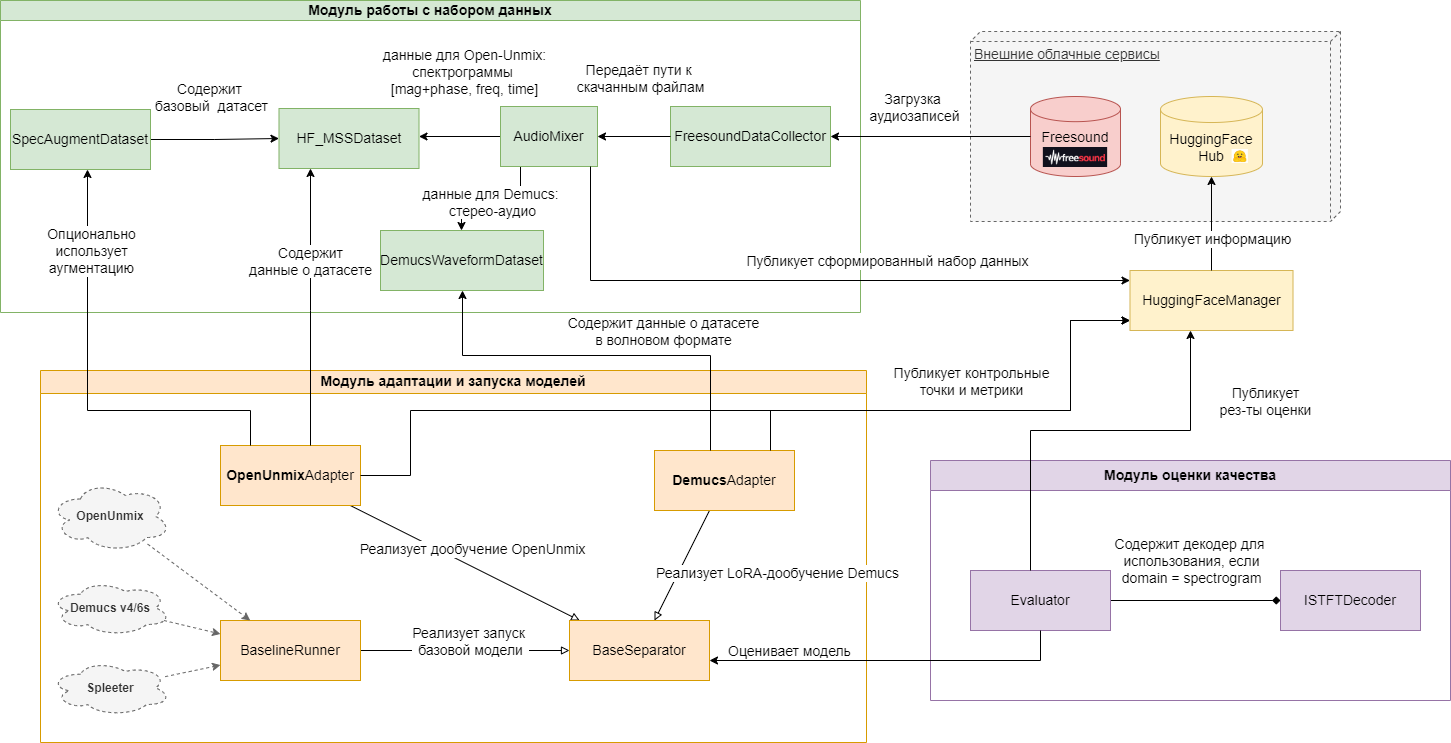
\includegraphics[width=1\textwidth]{figures/диаграмма классов сокр.png}
	\caption{Диаграмма взаимодействия модулей системы дообучения. Авторский материал}
	\label{fig:pipeline}
\end{figure}

Диаграмма классов (рисунки \ref{fig:diagclass1} и \ref{fig:diagclass2}) отражает модульную архитектуру разработанной системы, а также детализирует
состав классов в каждом модуле.
Модуль работы с набором данных содержит как логику сбора и подготовки данных для использования при дообучении базовых моделей 
(классы \texttt{FreesoundDataCollector}, \texttt{AudioMixer}), так и классы для работы уже в экспериментальной части системы 
(классы \texttt{HF\_MSSDataset}, \texttt{DemucsWaveformDataset} и \texttt{SpecAugmentDataset}). Класс \texttt{FreesoundDataCollector} 
реализует интерфейс загрузки аудио по тегам через API, а \texttt{AudioMixer} выполняет синтез миксов с заданным соотношением 
громкости источников. Для спектральных моделей класс \texttt{HF\_MSSDataset} обеспечивает предвычисление STFT и возврат тензоров 
магнитуды/фазы, тогда как \texttt{DemucsWaveformDataset} подготавливает сырые временные сигналы фиксированной длины для временных 
архитектур. Класс \texttt{SpecAugmentDataset}, реализующий паттерн Декоратор, применяет случайное маскирование по частоте и 
времени к тренировочным данным. Реализация классов модуля представлена в листинге~\ref{lst:module_dataset}.

Модуль обучения и адаптации моделей построен на едином базовом интерфейсе (класс \texttt{BaseSeparator}), 
который задает общие правила процесса обучения. На его основе созданы конкретные реализации для разных архитектур. 
Например, класс \texttt{OpenUnmixAdapter} управляет полным циклом дообучения рекуррентной сети Open-Unmix.
Он использует оптимизатор AdamW и планировщик скорости обучения CosineAnnealingLR, а также поддерживает работу с 
аугментированными данными. 
Для модели Demucs разработан класс \texttt{DemucsAdapter}. Он реализует эффективную настройку с помощью метода LoRA, 
внедряя адаптеры только в целевые линейные слои. Для ускорения работы и экономии видеопамяти здесь также предусмотрена 
поддержка смешанной точности FP16 и обучение на уменьшенных подвыборках данных. 
Класс \texttt{BaselineRunner} предоставляет интерфейс для запуска предобученных моделей без какого-либо изменения их весов, 
что необходимо для сравнения их работы с дообученными версиями. Реализация этих классов показана в листинге~\ref{lst:module_train}.

\begin{figure}[h!]
	\centering
	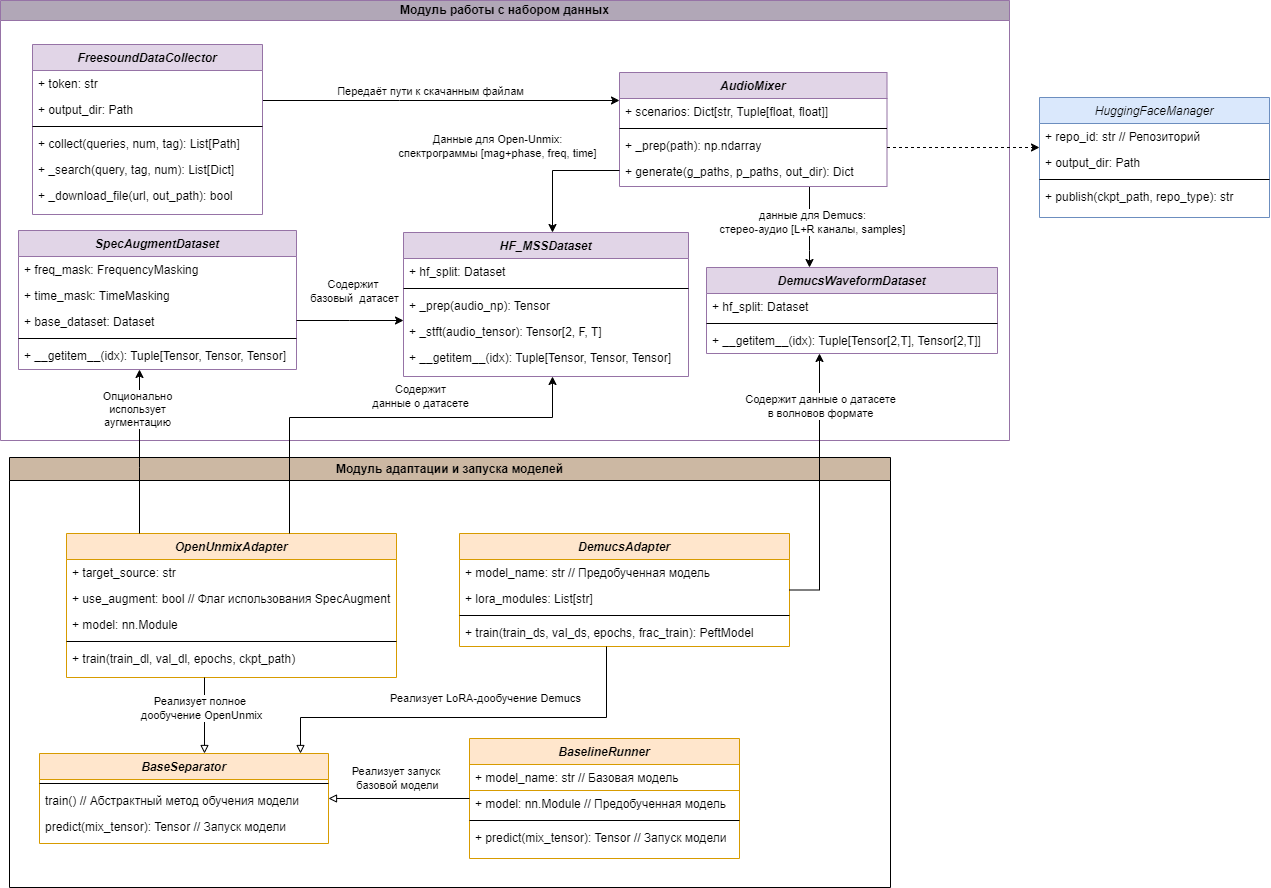
\includegraphics[width=1\textwidth]{figures/диаграмма классов (датасет+модели).png}
	\caption{Диаграмма классов. Модуль работы с набором данных и модуль адаптации и запуска моделей. Авторский материал}
	\label{fig:diagclass1}
\end{figure}

Модуль оценки качества содержит как основные классы для расчёта метрик и публикации результатов (классы \texttt{UnifiedEvaluator},
\texttt{HuggingFaceManager}) , так и вспомогательные классы для восстановления аудиосигнала из спектрального представления 
(класс \texttt{ISTFTDecoder}). Класс \texttt{ISTFTDecoder} выполняет обратное оконное преобразование Фурье с применением окна Ханна для
корректного восстановления временного сигнала из магнитуды и фазы. 
Класс \texttt{UnifiedEvaluator} реализует конвейер запуска моделей: переводит модель в режим оценки, выполняет прямой проход на 
тестовой выборке, рассчитывает метрики стандарта BSS Eval (SDR, SIR, SAR, SI-SDR) через библиотеку mir\_eval и фиксирует время выполнения. 
Реализация основных классов модуля представлена в листинге~\ref{lst:module_eval}.
Класс \texttt{HuggingFaceManager} отвечает за публикацию артефактов исследования: адаптированных контрольных точек моделей, подготовленных наборов данных, метрик качества
и сопроводительной документации в репозиторий Hugging Face Hub, обеспечивая открытость и воспроизводимость результатов. Реализация класса представлена в листинге ~\ref{lst:module_huggingface}.

\begin{figure}[h!]
	\centering
	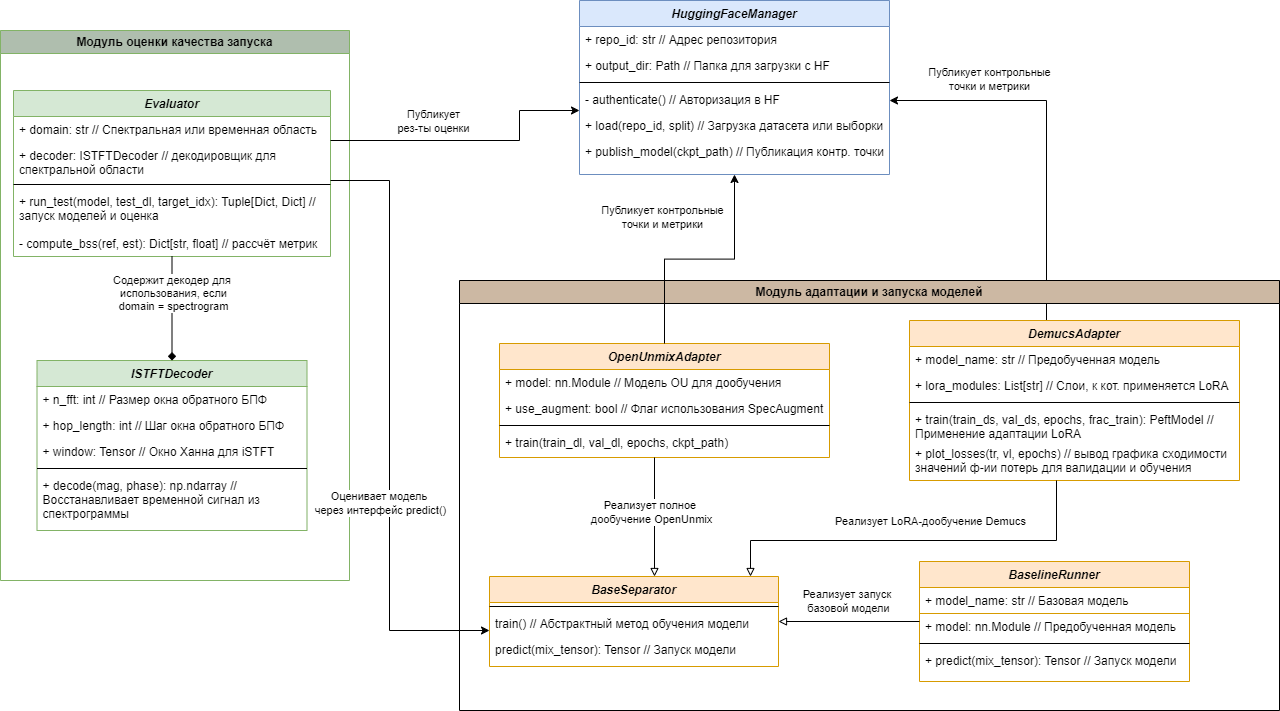
\includegraphics[width=1\textwidth]{figures/диаграмма классов (модели + оценка).png}
	\caption{Диаграмма классов. Модуль оценки качества запуска, класс взаимодействия с сервисом HuggingFace и модуль адаптации и запуска моделей. Авторский материал}
	\label{fig:diagclass2}
\end{figure}

\subsection{Модуль сбора и подготовки данных}

Особый интерес в контексте данной задачи представляет извлечение гармонических инструментов с высоким частотным 
перекрытием, таких как фортепиано и акустическая гитара, поскольку их совместное звучание формирует сложные 
спектральные коллизии ~\cite{piano_guitar_sep}, требующие от модели способности различать особые паттерны, а не полагаться лишь на 
грубую частотную фильтрацию.

Готовые эталонные наборы данных, такие как MUSDB18 ~\cite{MUSDB18} или Slakh2100 \cite{Slakh2100}, не предоставляют достаточного количества материалов 
для решения этой задачи: данные инструменты в них либо отсутствуют, либо сгруппированы в общие категории без 
отдельных чистых дорожек. В связи с этим был сформирован собственный размеченный набор на основе данных из открытых источников.
Для этого требовалось найти отдельные свободно размещённые файлы аудио с отдельно записанным звуком гитары и отдельно пианино,
затем с использованием программных средств их смешать между собой в разных комбинациях, чтобы получить разнообразие в наборе данных, 
сформировать выборки на два этапа дообучения (обучение и валидация), а также тестовую.

Кроме формирования набора данных, модуль отвечает за его публикацию во внешний сервис, а также за отдельную логику
по приведению набора к формату, который каждая из моделей могла бы получать на вход. 

Помимо сборки и разделения данных, модуль реализует функцию стандартизации. Для обеспечения совместимости с отличающимися
архитектурами предусмотрена адаптация формата входных данных: преобразование в спектрограммы для спектральной модели
Open-Unmix и поддержание временного формата для сети Demucs.
Завершающим этапом работы модуля является публикация готового набора данных во внешний сервис для воспроизводимости всех этапов 
(т.к. сессии среды Google Colab не позволяют дольше часа хранить в локальном хранилище данные).

\subsubsection{Загрузка исходных аудиозаписей. Клиент взаимодействия с сервисом Freesound}

Для формирования набора данных было решено использовать отдельные аудиозаписи гитары и пианино.
На начальном этапе рассматривалась возможность искусственной генерации аудиозаписей программными средствами.
Была проведена серия экспериментов по синтезу композиций гитары и пианино с использованием библиотек цифровой 
обработки сигналов (librosa, pydub, midiutil). Однако после проведения экспертной оценки сгенерированных записей
оказалось, что они не являются пригодными, так как на слух аудиодорожки звучали искусственно и 
звук не был похож на исходные музыкальные инструменты, поэтому этот путь оказался тупиковым.
Запись живых музыкантов также не подходила: это требовало бы студийного оборудования и значительных временных затрат,
которых в рамках исследования было недостаточно.

Поэтому было решено прибегнуть к использованию внешнего сервиса. Главными критериями выбора были открытый и бесплатный 
доступ к материалам. Выбор остановился на сервисе Freesound, который является открытым крупным репозиторием пользовательских 
аудиозаписей, распространяемых под свободными лицензиями. 
Наличие у сервиса официального программного интерфейса позволило автоматизировать поиск и скачивание нужных файлов через 
реализацию инстеграции в стиле REST API.

На рисунке \ref{fig:dataset-sd} отображена диаграмма последовательности процесса формирования набора данных через интерфейс сервиса Freesound.
\begin{figure}[h!]
	\centering
	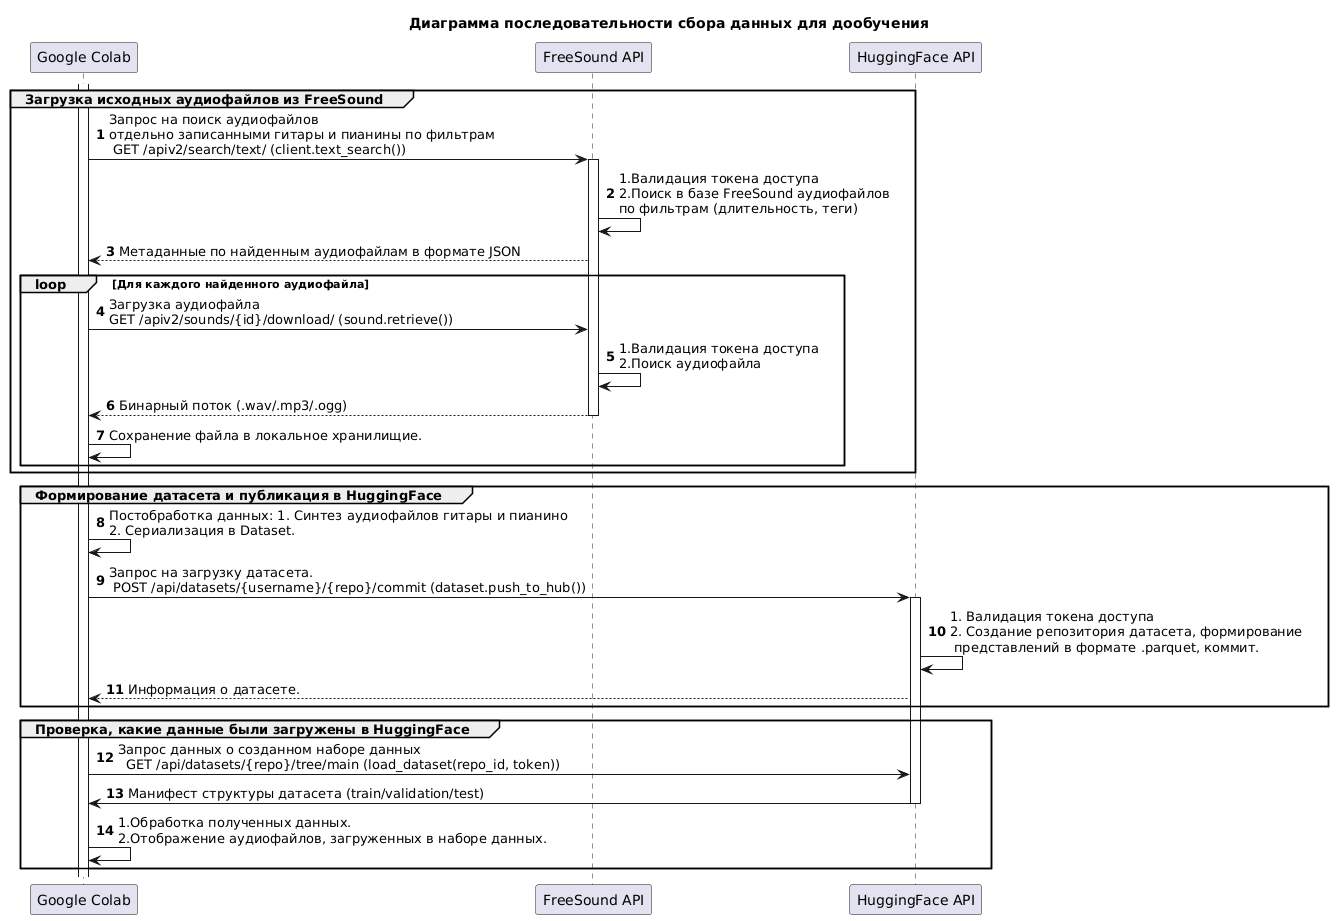
\includegraphics[width=1\textwidth]{figures/dataset/dataset.png}
	\caption{Диаграмма последовательности процесса формирования набора данных. Авторский материал}
	\label{fig:dataset-sd}
\end{figure}

Для работы с программным интерфейсом сервиса Freesound требовалась авторизация при выполнении каждого запроса.
После регистрации на сайте был получен уникальный ключ доступа (токен), который передавался в заголовке каждого HTTP-запроса.

Процесс сбора начинался с поиска записей по заданным критериям.
Для этого отправлялся GET-запрос по маршруту GET /apiv2/search/text/ (в реализации библиотеки freesound-api метод 
соответствует функции text\_search).

Параметры, по которым велся отбор аудиофайлов, подробно описаны в таблице~\ref{tab:freesound_search_params}.
\begin{longtable}{|l|>{\raggedright\arraybackslash}p{7cm}|>{}p{6.5cm}|}
	\caption{Параметры метода поиска аудиозаписей сервиса Freesound}
	\label{tab:freesound_search_params} \\
	\hline
	\textbf{Параметр} & \textbf{Значение} & \textbf{Назначение} \\
	\hline
	\endfirsthead
	
	\hline
	\textbf{Параметр} & \textbf{Значение} & \textbf{Назначение} \\
	\hline
	\endhead

	\hline
	\endfoot

	\hline
	\endlastfoot

	query & Для гитары: <<guitar>> \allowbreak <<acoustic guitar>> \allowbreak <<guitar clean>>. Для~пианино: <<piano>>, <<piano classic>>, <<piano jazz>> & Текстовые вариации запросов для поиска записей музыкальных инструментов. \\
	\hline
	filter & tag:"solo" \allowbreak duration:[5 TO 15] & Тег solo устанавливает ограничение на записи с аккомпанементом. Тег duration устанавливает границы длительности в 5–15 секунд. \\
	\hline
	fields & id, name, previews, license, download & Минимизация объёма ответа за счёт запроса только необходимых полей. \\
	\hline
	page\_size & 20–50 & Контроль количества результатов на один запрос для соблюдения ограничений частоты запросов к серверу. \\
	\hline
\end{longtable}

После определения списка подходящих аудиофайлов выполнялась их загрузка в локальное хранилище Google Colab.
Загрузка исходных файлов осуществлялась по маршруту GET /apiv2/sounds/\{id\}/download/ (в реализации библиотеки freesound-api --- функция retrieve\_preview), 
возвращающий бинарный поток аудиофайла в ответ на GET-запрос.

При сохранении файлу присваивалось <<безопасное>> наименование без недопустимых символов.
Также выполнялась проверка формат загружаемого файла: сохранялись только файлы с расширениями .wav, .mp3 или .ogg, а остальные переименовывались в .wav. 
Таким образом был обеспечен единый стандарт данных для дальнейшей обработки.

В результате выполнения алгоритма отбора аудиотреков было загружено 27 аудиофайлов 
с гитарой и 16 с пианино. Каждый из них далее требовалось смешать между собой с разной громкостью.

\subsubsection{Синтез аудиомиксов из загруженных айдиофайлов и постобработка}
% : все аудиозаписи нормализуются к диапазону $[-1, 1]$,
%  приводятся к единой частоте дискретизации 44,1~кГц и нарезаются на фиксированные сегменты длительностью 4~секунды

Логика по синтезу сырых аудиофайлов в аудиомиксы и формирование выборок была реализована в классе \texttt{AudioMixer}.
На основе загруженных аудиодорожек был сформирован набор аудиомиксов путём линейного 
суммирования сигналов с различными соотношениями громкости (равная громкость, гитара громче, пианино громче),
что позволило смоделировать реалистичные сценарии спектрального перекрытия в диапазоне 200–500 Гц (критическом для тембрового различения данных инструментов).
Сценарии балансировки громкости источников в аудиомиксах были заданы следующие:
\begin{enumerate}[label=\arabic*)]
	\item \texttt{balanced} --- равнозначное усиление гитары и пианино (коэффициенты громкости сбалансированы: и для аудиофайла с гитарой, и с пианино применялся множитель 0.8);
	\item \texttt{guitar\_loud} --- доминирование гитары в миксе (коэффициенты: для гитары --- 1.0, для пианино --- 0.5);
	\item \texttt{piano\_loud} — доминирование пианино (коэффициенты: для пианино --- 1.0, для гитары --- 0.5).
\end{enumerate}
Благодаря такому подходу модель учится работать с разной громкостью инструментов и лучше справляется с реальными 
аудиомиксами, где баланс между инструментами может сильно меняться.

Перед тем как смешивать звуки, каждый файл проходит подготовку в методе \texttt{prepare\_audio} класса \texttt{AudioMixer}:
\begin{enumerate}[label=\arabic*)]
	\item Приведение к единой частоте дискретизации. 
	Все сигналы конвертируются в частоту $f_s = 44\,100$~Гц с помощью библиотеки librosa
	Это необходимо, чтобы при одинаковых параметрах оконного преобразования Фурье ($N_{fft}=4096$, $hop=1024$) 
	все спектрограммы имели одинаковый размер по оси ординат (где отложены частоты) --- иначе модель Open-Unmix не сможет 
	работать с пакетами данных фиксированной формы.
	\item Все записи приводятся к длине ровно 4 секунды: если исходная запись короче 4 секунд, она дополняется нулевыми отсчётами (тишиной);
	если длиннее — берётся только первый 4-секундный кусок. Это нужно, чтобы все входные тензоры имели одинаковый размер и не возникало ошибок при их обработке.
\end{enumerate}

Метод \texttt{generate} перебирает все возможные комбинации загруженных дорожек гитары и пианино. 
Для каждой пары и каждого сценария громкости выполняются следующие действия:
\begin{enumerate}[label=\arabic*)]
	\item Смешивание сигналов. Сигналы умножаются на коэффициенты громкости и складываются:
		\begin{equation*}
			y_{\text{mix}} = \alpha_g \cdot y_g + \alpha_p \cdot y_p,
			\label{eq:audio_mixing}
		\end{equation*}
		где
			\begin{itemize}[label=$\bullet$, wide]
				\item $y_{\text{mix}}$ --- итоговый смешанный аудиосигнал;
				\item $y_g$, $y_p$ --- исходные сигналы гитары и пианино;
				\item $\alpha_g$, $\alpha_p$ --- коэффициенты, регулирующие громкость инструментов.
			\end{itemize}
	\item Нормализация громкости. Полученный из двух инструментов аудиосигнал масштабируется таким образом, чтобы его
	максимальное абсолютное значение амплитуды не превышало 1. Это предотвращает цифровые искажения сигнала и 
	гарантирует, что все значения отсчётов сигнала будут расположены в диапазоне $[−1,1]$.
	\item Вместе с полученным аудиомиксом сохраняются нормализованные версии отдельных инструментов-источников,
	которые далее будут использоваться как эталонные исходные источники при обучении и оценке качества разделения.
	\item Все выходные файлы получают структурированные имена вида \texttt{mix\_XXXX\_scenario\_role.wav}, 
	где \texttt{role} указывает на тип сигнала (mixture --- полученный аудиомикс, guitar --- источник-гитара, 
	piano --- источник-пианино). Такое именование файлов упрощает дальнейшую загрузку данных.
\end{enumerate}

\subsubsection{Состав и количество выборок}

Исходный набор данных был разделён на три выборки: обучающую, валидационную и тестовую в соотношении 70:15:15 (рисунок~\ref{fig:trainset}).

\begin{figure}[h!]
	\centering
	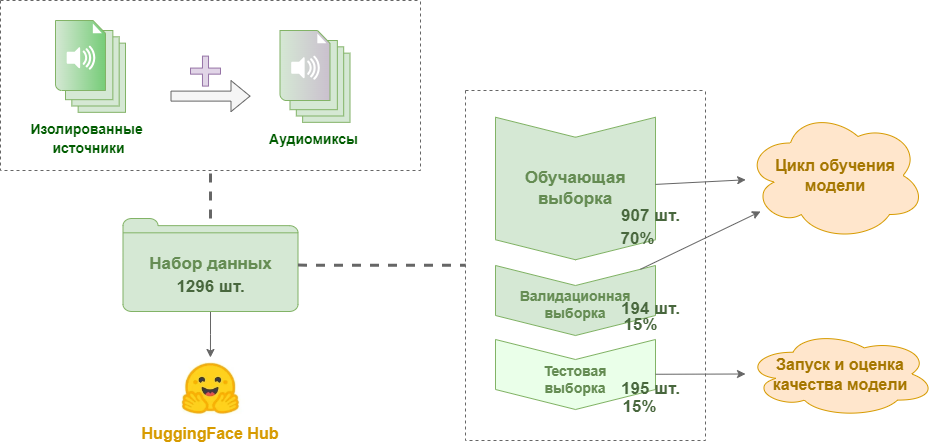
\includegraphics[width=1\textwidth]{figures/состав выборок.png}
	\caption{Структура разделения набора данных на обучающую, валидационную и тестовую выборки. Авторский материал}
	\label{fig:trainset}
\end{figure}

% Выжимка про типы выборок: https://habr.com/ru/articles/500196/

При разделении важно было, чтобы все миксы, сгенерированные из одной пары исходных файлов 
(гитара + фортепиано), попадали исключительно в одну выборку. Например, если из пары 
\texttt{guitar\_001.wav} и \texttt{piano\_001.wav} были созданы три микса с разной громкостью 
(сбалансированный, с доминированием гитары и с доминированием фортепиано), все три должны 
оказаться либо в обучающей, либо в тестовой выборке.
Это исключает ситуацию, когда модель обучается на одних вариантах громкости этих инструментов, 
а тестируется на других вариантах тех же самых записей. В противном случае модель могла бы 
<<запомнить>> конкретные ноты и тембр, что привело бы к завышенным метрикам качества и 
некорректной оценке её обобщающей способности.

Процедура разделения реализована в виде двухэтапного алгоритма с фиксацией состояния генератора 
псевдослучайных чисел (\texttt{random\_state=42}) для обеспечения воспроизводимости результатов. 
На первом этапе исходный набор аудиомиксов разделяется на обучающую выборку (70\%) и отложенную часть (30\%). 
На втором этапе отложенная часть аудиомиксов делится пополам на валидационную и тестовую 
(по 15\% от общего объёма данных).

Для обеспечения сбалансированности каждой выборки применялось пропорциональное разделение по типу 
сценария смешивания аудиомиксов: сбалансированные инструменты (\texttt{balanced}), 
с преобладанием гитары (\texttt{guitar\_loud}) и с акцентом на пианино (\texttt{piano\_loud}).
Это гарантирует, что все три категории аудиомиксов равномерно представлены в каждой выборке.
Такой подход позволил сохранить сходное распределение соотношений громкости в выборках 
на всех этапах эксперимента.

На листинге \ref{lst:split_sets} представлена логика разделения всех смешенных аудиоисточников 
на три основные выборки для применения их далее на всех шагах дообучения и тестирвания работы моделей.

\begin{lstlisting}[caption={Разделение всех смешенных аудиоисточников на три основные выборки}, label={lst:split_sets}, language=Python]
RANDOM_SEED = 42
np.random.seed(RANDOM_SEED)

# Этап 1: выделение обучающей выборки (70%) и отложенной части (30%)
idx_train, idx_temp = train_test_split(
    all_indices, test_size=0.30, random_state=RANDOM_SEED, stratify=scenario_labels
)

# Этап 2: разделение остатка на тест и валидацию.
# каждая составит по 15% от исходного объёма данных
idx_val, idx_test = train_test_split(
    idx_temp, test_size=0.50, random_state=RANDOM_SEED, stratify=scenario_labels[idx_temp]
)
\end{lstlisting}

Итогом работы модуля является структурированный словарь метаданных, содержащий пути к сгенерированным 
файлам, информацию о применённом сценарии и принадлежность к выборке. 
Данная структура передаётся в конвейер загрузки данных. 
Поскольку все подвыборки получены из одного набора данных и разделены с сохранением пропорций, 
распределение ключевых признаков (типов смешения и громкостных соотношений) остаётся статистически 
однородным. Это исключает ситуацию, когда обучающие и проверочные данные существенно различаются 
по составу, что гарантирует объективность сравнительного анализа моделей.

Тренировочная выборка, содержащая 910 файлов, использовалась для выполнения обновления параметров модели:
на этих данных вычислялась функция потерь и выполнялся шаг оптимизатора, что позволяло модели адаптироваться
к специфике выделения гитары как аудиоисточника.

Валидационная выборка, включающая 194 файлов, применялась для контроля процесса обучения:
после каждой эпохи на ней рассчитывалась ошибка валидации (val\_loss), что позволяло реализовать 
механизм ранней остановки и отобрать контрольную точку модели с наилучшей обобщающей способностью.

Итоговая тестовая выборка содержала 195 независимых треков, на которых проводилась финальная оценка 
всех метрик качества (SDR, SIR, SAR, SI-SDR). 
Несмотря на относительно небольшой объём, её размер является статистически достаточным для надёжной 
оценки качества разделения источников. 

\subsubsection{Интеграция с платформой HuggingFace}

Для обеспечения воспроизводимости экспериментов, сохранения версий файлов моделей и наборов данных,
в системе реализована интеграция с облачным сервисом HuggingFace Hub.
Данный сервис предоставляет специализированные репозитории, оптимизированные для хранения и управления артефактами машинного обучения.
Интерфейс для аутентификации, выгрузки и загрузки подготовленных данных и дообученных моделей в сервис HuggingFace
реализоан в классе \texttt{HuggingFaceManager}, а логика подготовки данных в специальный формат
для последующей передачи их в модели вынесена в класс \texttt{HF\_MSSDataset}.

\par\textbf{Публикация и загрузка набора данных в сервис HuggingFace}
\label{sec:huggingface}

Процесс публикации данных выстроен в виде последовательного конвейера взаимодействия 
объектов классов \texttt{AudioMixer} и \texttt{HuggingFaceManager}.
Сначала метод \texttt{generate} класса \texttt{AudioMixer} формирует стандартный Python-словарь 
(\texttt{Dict[str, List]}), содержащий пути к сформированным файлам аудиомиксов в формате \texttt{.wav}
и соответствующую разметку по выборкам.

Затем этот словарь передаётся в экземпляр класса \texttt{HuggingFaceManager}.
На этом этапе данные преобразуются в формат Parquet --- стандартный для платформы 
Hugging Face столбцовый формат, обеспечивающий высокую степень сжатия. 
Для корректной интерпретации звуковых файлов к соответствующему столбцу применяется класс Audio 
из библиотеки datasets, который настраивает автоматическое декодирование аудиофайлов при обращении к элементам набора.  

Публикация сформированного набора данных в облачный репозиторий осуществляется через метод 
\texttt{publish\_dataset} класса \texttt{HuggingFaceManager}. Он принимает на вход словарь DatasetDict, 
содержащий именованные выборки (train, val, test).
Процедура публикации включает следующие этапы:
\begin{enumerate}[label=\arabic*)]
	\item Аутентификация. Выполняется авторизация в сервис Hugging Face Hub с использованием API-токена. Предварительно была 
	осуществлена регистрация в сервис с последующей регистрацией персонального токена доступа.
	\item Валидация и конвертация. Если данные переданы в виде стандартного словаря, они автоматически конвертируются в формат DatasetDict.
	\item Загрузка набора данных. Вызывается метод push\_to\_hub, который загружает все выборки в 
	указанный репозиторий, сохраняя метаданные (пути к файлам, сценарии смешения, принадлежность к выборке).
\end{enumerate}

По завершении операции модуль возвращает URL-ссылку на опубликованный набор данных, что позволяет повторно использовать его в 
других экспериментах или передать для независимого воспроизведения.

Для загрузки опубликованного набора данных в среду Google Colab реализован 
метод \texttt{load} в классе \texttt{HuggingFaceManager}, который обеспечивает выборочную загрузку отдельных выборок или полного набора.
Также метод поддерживает режим потоковой передачи, при котором файлы считываются по мере необходимости 
без полного скачивания в хранилище.

Для обработки в подходящий формат загруженного набора данных реализован класс \texttt{HF\_MSSDataset},
наследующий интерфейс torch.utils.data.Dataset. Класс решает две основные задачи:
\begin{enumerate}[label=\arabic*)]
	\item Загрузка и стандартизация аудиофайлов. Метод обращения к элементу набора данных \texttt{\_\_getitem\_\_} (то есть получение одной из трех выборок по ключу train/validation/test)
	извлекает из загруженной выборки по тройке аудиофайлов: сам аудиомикс и два файла с инструментами-источниками
	и приводит к единому формату (конвертация numpy-массива в тензор torch формы [1, T]).
	При этом автоматически аудиофайлы декодируются из Parquet-формата в NumPy-массивы, содержащие амплитуды аудиосигнала.
	\item Применение ОПФ. После приведения к единой размерности выполняется динамическое вычисление оконного преобразования Фурье
	в методе \_stft. Комплексный спектр разделяется на магнитудную и фазовую компоненты, которые объединяются в тензор 
	формы $[2, F, T]$ (где первое измерение соответствует каналам (магнитуда, фаза), $F = 2049$ --- число частотных интервалов, $T$ --- число временных интервалов).
	Такой подход позволяет хранить в облаке только временные сигналы, что экономит пространство локального хранилища, 
	а спектральные представления вычислять непосредственно в процессе обучения.
\end{enumerate}

\par\textbf{Публикация и загрузка моделей из сервиса HuggingFace}

Публикация дообученных моделей и сопутствующих им артефактов реализуется через метод 
\texttt{publish\_model}, который автоматизирует процесс выгрузки результатов исследования в 
репозиторий сервиса HuggingFace типа <<model>>.

При публикации выполняются следующие действия:
\begin{enumerate}[label=\arabic*)]
	\item Если указанный репозиторий не существует, он создаётся автоматически с заданными параметрами доступа.
	\item Файл с весами модели (.pt, .safetensors) загружается в корень репозитория.
	\item При наличии файла с результатами оценки в локальном хранилище (metrics.json) он также выгружается для документирования качества модели.
	\item Модуль автоматически формирует файл README.md в стандарте Hugging Face, содержащий: метаданные (лицензия, теги), краткое описание модели, пример кода для запуска модели.
\end{enumerate}


\subsection{Адаптация Open-Unmix для полного дообучения}
Процесс адаптации модели Open-Unmix организован в виде двух логически разделённых режимов работы: контура дообучения и контура валидации, 
что обеспечивает контроль качества на каждом этапе и предотвращает переобучение. 
Валидационный режим выполняется после завершения каждой эпохи обучения, что обеспечивает контроль качества на каждом этапе и 
предотвращает переобучение. Несмотря на то, что оба режима используют общую архитектуру модели и функцию потерь,
они различаются по поведению: в режиме обучения применяется спектральное маскирование, вычисление градиентов и обновление весов, 
тогда как в режиме валидации модель работает в режиме запуска без изменения параметров.

На рисунке \ref{fig:train-ou} представлена схема реализации алгоритма дообучения модели OpenUnmix с разделением на два контура -- дообучение и валидации.

\begin{figure}[h!]
	\centering
	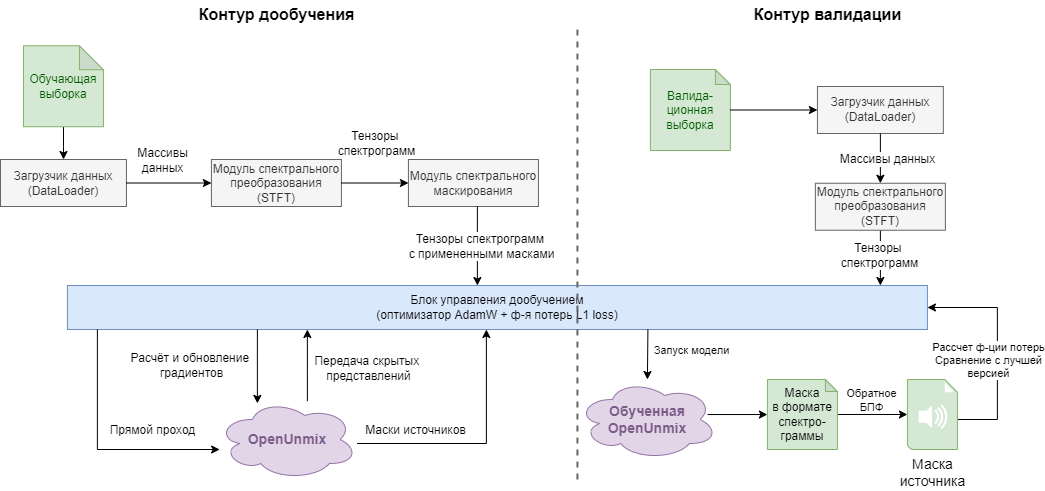
\includegraphics[width=1\textwidth]{figures/конвейер обучения open unmix.png}
	\caption{Схема реализации алгоритма дообучения модели OpenUnmix. Авторский материал}
	\label{fig:train-ou}
\end{figure}

% В рамках контура дообучения реализован итеративный процесс обновления параметров нейросетевой архитектуры на основе обучающей выборки.
% Обучающая выборка поступает в систему через класс  , использующий ранее описанный адаптер HF_MSSDataset, который выполняет потоковую загрузку аудио из Hugging Face Hub, стандартизацию длительности (4 секунды) и динамическое вычисление STFT с параметрами, описанными в разделе 2.X.

\subsubsection{Контур дообучения}
Процесс дообучения модели Open-Unmix начинается с загрузки аудиофайлов из обучающей выборки. 
Для этого используется стандартный класс DataLoader из библиотеки torch.utils.data, который разбивает данные на небольшие 
пакеты, перемешивает их и загружает в несколько потоков для ускорения работы.

Полученные сырые аудиосигналы затем преобразуются в спектрограммы.
Этот этап работает через взаимодействие классов \texttt{HuggingFaceManager} и \texttt{HF\_MSSDataset},
которые были описаны в разделе~\ref{sec:huggingface}.
Они переводят временной сигнал в частотно-временное представление, готовое для подачи в нейронную сеть.

Перед началом обучения загружается предобученная модель OpenUnmix (версия umxhq) из репозитория 
sigsep/open-unmix-pytorch с помощью механизма torch.hub. 
Поскольку задача дообучения --- выделение гитары, производится следующая замена: перенастраиваем выход модели на 
канал guitar и размораживаются все параметры сети (устанавливается \texttt{requires\_grad=True}), 
чтобы модель могла полностью подстроиться под новые данные. 
Все вычисления автоматически выполняются на доступном графическом или центральном процессоре.

Для обучения настраиваются следующие компоненты:
\begin{itemize}[label=$\bullet$, wide]
	\item оптимизатор AdamW с начальной скоростью обучения $lr = 10^{-4}$ и коэффициентом регуляризации $\text{weight\_decay} = 10^{-3}$;
    \item планировщик скорости обучения CosineAnnealingLR, который плавно снижает скорость обучения до минимального значения $lr_{\min} = 10^{-5}$;
    \item функция потерь $L_1$ (среднее абсолютное отклонение), оценивающая разницу между предсказанием и эталоном.
\end{itemize}

Для каждого пакета данных из обучающей выборки выполняется следующий цикл:
\begin{enumerate}[label=\arabic*.]
    \item Инициализация тензоров. Входной аудиомикс и эталонный сигнал переносятся в память вычислительного устройства (GPU или CPU) с помощью метода \texttt{.to(self.device)}.
    \item Очистка градиентов. Вызывается метод opt.zero\_grad, который очищает буфер градиентов, предотвращая их накопление с предыдущих итераций.
    \item Прямой проход. Спектрограмма аудиомикса подаётся на вход модели, предсказывающей аудиоисточник.
    \item Вычисление значений функции потерь. Качество разделения оценивается через функцию потерь: вычисляется $L_1$-расстояние (средняя абсолютная ошибка, MAE) между сгенерированным моделью сигналом источника и эталоном.
    \item Обратное распространение ошибки. При вызове метода loss.backward вычисляются градиенты функции потерь по всем обучаемым параметрам модели, двигаясь от выходного слоя к входному.
    \item Стабилизация обучения. Для предотвращения экспоненциального роста величин градиентов применяется их нормировка с пороговым значением $1.0$ посредством вызова 
    функции clip\_grad\_norm.
    \item Обновление весов. Вызывается метод opt.step, который обновляет веса модели в соответствии с вычисленными градиентами и правилами выбранного алгоритма оптимизации.
\end{enumerate}

В конце каждой эпохи модель переключается в режим оценки model.eval(), и через неё прогоняется валидационную выборку без расчета градиентов 
(см. подраздел <<Контур валидации>> ниже).
Затем рассчитывается значение средней $L_1$-ошибки по всем пакетам и информация выводится на панель вывода. 
Текущее состояние модели (веса, номер эпохи, значение ошибки на валидации) сохраняется в файл контрольной точки (\texttt{.pt}).

\subsubsection{Контур валидации}
На этом этапе модель не учится --- мы только смотрим, насколько хорошо она справляется с данными, которых не видела во время обучения. Вот как это устроено:


Чтобы следить за процессом обучения и предотвращения переобучения, после каждой эпохи запускается проверка модели на валидационной выборке, 
На этом этапе модель не учится --- этап нужно для проверки, насколько хорошо она справляется с данными, которых не видела во время обучения. 
Детальные шаги валидации описаны ниже:
\begin{enumerate}[label=\arabic*)]
    \item Подготовка к проверке. Контур активируется после завершения каждой эпохи обучения. Модель переключается в режим оценки, что отключает случайные элементы и делает результаты предсказуемыми и воспроизводимыми.
    \item Обработка данных без обучения. Для каждого пакета данных валидационной выборки выполняются следующие действия:
    \begin{itemize}[label=$\bullet$, wide]
        \item Тензоры аудиомикса \texttt{mix} и эталонного аудиофайла с гитарой перемещаются на вычислительное устройство (видеокарту или процессор);
        \item Аудиомикс передается через модель self.model(mix) и на выходе модель выдает результат разделения;
        \item Вычисляется $L_1$-ошибка между предсказанным результатом и эталоном;
        \item Значение ошибки сохраняется для последующего усреднения.
    \end{itemize}
    \item Подсчет итоговой метрики. После прохода по всей валидационной выборке:
    \begin{itemize}[label=$\bullet$, wide]
        \item вычисляется среднее значение ошибки по всем пакетам: $val\_loss = \frac{1}{N} \sum_{i=1}^{N} \mathrm{loss}_i$;
        \item результат выводится в консоль в формате \texttt{Ep \{e\} | Val: \{v:.4f\}};
        \item полученная метрика используется, чтобы понять, сходится ли модель и выбрать оптимальную контрольную точку для финального тестирования.
    \end{itemize}
\end{enumerate}

\subsubsection{Спектральное маскирование}

Для исследования изменения уровня устойчивости модели и снижения риска переобучения на малых выборках в логику дообучения
добавлен опциональный модуль спектральной аугментации (или маскирования), реализованный в классе SpecAugmentDataset. Данный компонент применяется
только к обучающей выборке.

Класс \texttt{SpecAugmentDataset} реализует интерфейс torch.utils.data.Dataset и выполняет преобразования в соответствии с шагами:
\begin{enumerate}[label=\arabic*)]
	\item Компоненты извлекаются из базового набора данных (\texttt{self.base\_dataset}), который передаётся в конструктор \texttt{SpecAugmentDataset} и оборачивается им.
	в качестве базового набора данных используется класс \texttt{HF\_MSSDataset}, который осуществляет потоковую загрузку аудиоданных из репозитория Hugging Face 
	Hub и динамическое вычисление ОПФ. Для каждого индекса idx метод \texttt{\_\_getitem\_\_} базового набора данных возвращает три спектрограммы: аудиомикс,
	эталонную гитару и эталонное пианино, каждая из которых представлена в виде тензора [2, F, T] (каналы: магнитуда/фаза).
	\item С вероятностью \texttt{p\_apply=0.5} активируется процедура маскирования; в остальных 50\% случаев данные передаются без изменений, что обеспечивает разнообразие пакетов данных.
	\item Сам процесс спектрального маскирования представляет собой преобразование, применяемо к магнитуде входного сигнала (\texttt{mix[0]}):
		\begin{itemize}[label=$\bullet$, wide]
			\item Тензор магнитуды временно расширяется до размерности [1, F, T] для совместимости с torchaudio.transforms;
			\item Применяется частотное маскирование (FrequencyMasking) с параметром \texttt{freq\_mask\_param=32}: случайно выбирается начальная частота, и полоса шириной до 32 частотных интервалов зануляется;
			\item Применяется временное маскирование (TimeMasking) с параметром \texttt{time\_mask\_param=64}: случайно выбирается начальный фрейм, и отрезок длиной до 64 временных интервалов зануляется;
			\item Модифицированная магнитуда возвращается в исходную форму $[F, T]$ и записывается обратно в $mix[0]$.
		\end{itemize}
	\item Эталонные сигналы гитары и пианино не модифицируются. 
\end{enumerate}

Модуль спроектирован как обёртка (паттерн <<Декоратор>>) над базовым набором данных, что позволяет гибко включать или 
отключать аугментацию без изменения кода обучения (листинг~\ref{lst:decorator}).
\begin{lstlisting}[caption={Пример применения класса BaseDataset для инициализации наборов данных с аугментацией и без неё}, label={lst:decorator}, language=Python]
# Базовая инициализация (например, для валидации или тестирования)
train_ds = BaseDataset(...)
# Инициализация с применением аугментации (для обучения)
train_ds = SpecAugmentDataset(BaseDataset(...), p_apply=0.5, freq_mask_param=32, time_mask_param=64)
\end{lstlisting}

% # Вариант 1: Без аугментации (baseline)
% train_loader = DataLoader(
%     HF_MSSDataset(ds["train"]),  # Просто спектрограммы
%     batch_size=2
% )

% # Вариант 2: С аугментацией (улучшенная модель)
% base_ds = HF_MSSDataset(ds["train"])
% aug_ds = SpecAugmentDataset(
%     base_ds,           # ← Передаём базовый датасет ВНУТРЬ обёртки
%     p_apply=0.5,       # 50% вероятность аугментации
%     freq_mask_param=32, # Маскируем до 32 частотных бинов
%     time_mask_param=64  # Маскируем до 64 временных фреймов
% )
% train_loader = DataLoader(aug_ds, batch_size=2)

% # Для валидации аугментация НЕ нужна!
% val_loader = DataLoader(HF_MSSDataset(ds["validation"]), batch_size=2)


В рамках данного исследования проведены две серии экспериментов:
\begin{enumerate}[label=\arabic*)]
	\item Базовая конфигурация: дообучение без применения спектрального маскирования;
	\item Конфигурация с регуляризацией: дообучение с активированным SpecAugmentDataset.
\end{enumerate}
Сравнение результатов этих запусков (представленное в главе 3) позволяет количественно оценить вклад аугментации в улучшение обобщающей способности модели.


% \subsubsection{Полное дообучение Open-Unmix с аугментацией спектрограмм}



% \begin{lstlisting}[caption={}, label={lst:openunmix-aug}, language=Python]
% import torch, random, torchaudio
% from torch.utils.data import Dataset, Subset, DataLoader

% class SpecAugmentDataset(Dataset):
%     def __init__(self, base_ds, p=0.5, fm=32, tm=64):
%         self.base, self.p = base_ds, p
%         self.fm, self.tm = torchaudio.transforms.FrequencyMasking(fm), torchaudio.transforms.TimeMasking(tm)
%     def __len__(self): return len(self.base)
%     def __getitem__(self, i):
%         m,g,p = self.base[i]
%         if random.random() < self.p:
%             m[0] = self.tm(self.fm(m[0].unsqueeze(0))).squeeze(0)
%         return m,g,p
% \end{lstlisting}



% Модификация под целевые классы: замена выходного слоя с 4 на 2 канала (пианино, гитара), адаптация функции потерь.
% Настройка гиперпараметров: выбор оптимизатора (AdamW), начального learning rate (1e-5–5e-5), размера батча, количества эпох, стратегии early stopping.
% Оптимизация под Colab: использование fp16, gradient_accumulation, выгрузка неактивных тензоров.
% Рекомендуемые элементы: Схема изменённого вычислительного графа; таблица гиперпараметров




\subsection{Дообучение модели Demucs методом LoRA}
Дообучение модели htdemucs v4 выполнено с применением метода низко-ранговой адаптации (LoRA — Low-Rank Adaptation). 
В отличие от классического полного обновления весов, при данном подходе базовые параметры всех свёрточных, трансформерных и
линейных слоёв остаются замороженными, а обучению подлежат только компактные адаптерные модули, внедряемые в целевые слои сети.

\subsubsection{Интеграция LoRA в архитектуру Demucs v4}

Вся логика адаптации модели Demucs реализована в классе \texttt{DemucsAdapter}, который наследует абстрактный интерфейс
\texttt{BaseSeparator} и предоставляет методы \texttt{train} и \texttt{predict} для обучения и вывода соответственно.
Наличие базового класса \texttt{BaseSeparator} позволяет системе работать с различными архитектурами (Open-Unmix, Demucs) 
через единый программный интерфейс, что обеспечивает гибкость при переключении между моделями без изменения кода конвейера.

На этапе инициализации \texttt{DemucsAdapter} сканирует вычислительный граф модели и выявляет все полносвязные 
слои (nn.Linear), присутствующие в блоках механизма внимания и прямой связи трансформерной части Demucs.
Именно эти слои признаны наиболее подходящими для применения низко-ранговой декомпозиции, так как они содержат 
основную долю обучаемых параметров и отвечают за проекцию признаков в пространства запросов, ключей и значений.
Имена этих слоёв сохраняются и передаются в конфигурацию библиотеки PEFT для последующего внедрения адаптеров. 

Внедрение адаптеров в вычислительный граф модели осуществляется с помощью функции get\_peft\_model 
из библиотеки Hugging Face PEFT.
На вход функции передаётся объект конфигурации LoraConfig, инициализированный следующими параметрами:
\begin{itemize}[label=$\bullet$, wide]
    \item r=8 --- ранг матриц адаптера, определяющий количество обучаемых параметров;
    \item lora\_alpha=16 --- коэффициент масштабирования, усиливающий вклад адаптерной поправки;
    \item lora\_dropout=0.05 --- вероятность отсева для предотвращения совместной адаптации признаков;
    \item target\_modules --- список выявленных ранее полносвязных слоёв.
\end{itemize}
Внутри библиотеки PEFT автоматически замораживает базовые веса модели и добавляет к каждому целевому слою 
пару линейных матриц ($A$ и $B$). 
В начале обучения матрица $B$ инициализируется нулями, что гарантирует: 
до первого шага оптимизации модель выдаёт в точности те же результаты, что и исходная предобученная версия,
без внесения случайных искажений.

На рисунке \ref{fig:demucs-train-archit} приведена схема архитектурных изменений в модели Demucs, описанных выше.

\begin{figure}[h!]
	\centering
	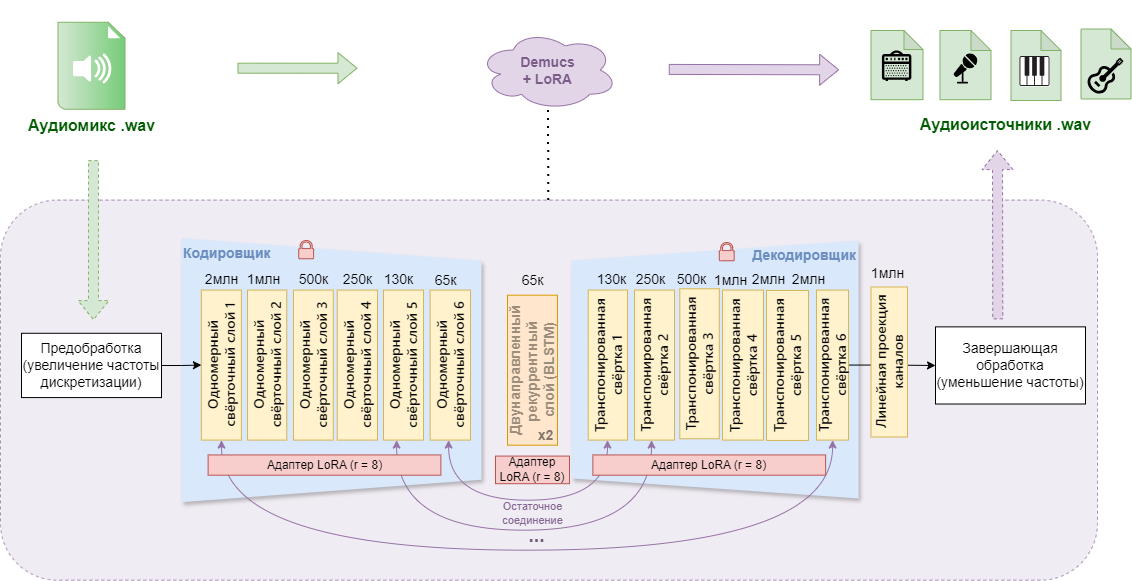
\includegraphics[width=1\textwidth]{figures/demucs доработка архитектуры.png}
	\caption{Архитектурные изменения в Demucs. Авторский материал}
	\label{fig:demucs-train-archit}
\end{figure}

Процесс дообучения модели Demucs v4 организован по аналогичной схеме, что и для архитектуры Open-Unmix: система 
включает два изолированных контура — контур дообучения и контур валидации (рисунок \ref{fig:demucs-train}).
Ключевое отличие заключается в том, что для Demucs применяется метод параметрически эффективной адаптации: 
сначала функция get\_pef\_model внедряет LoRA-адаптеры в вычислительный граф модели, замораживая базовые веса,
и только после этого запускается цикл оптимизации в методе \texttt{train\_lora}, который обновляет исключительно параметры
адаптерных матриц, оставляя неизменными 115 миллионов параметров предобученной сети.

\begin{figure}[h!]
	\centering
	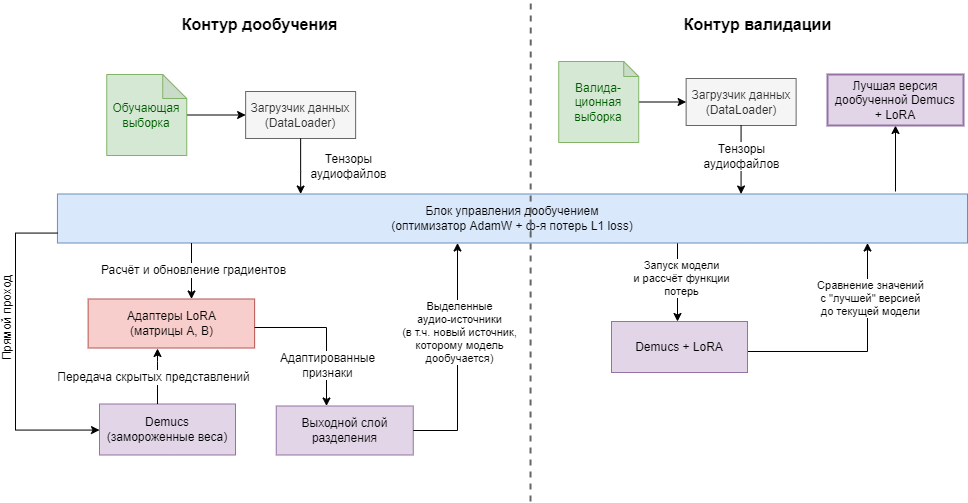
\includegraphics[width=1\textwidth]{figures/конвейер обучения demucs.png}
	\caption{Схема реализации алгоритма дообучения модели Demucs. Авторский материал}
	\label{fig:demucs-train}
\end{figure}


\subsubsection{Контур дообучения}

За процесс дообучения модели Demucs v4 отвечает класс \texttt{DemucsAdapter}. Он работает с данными, которые уже подготовил модуль работы с набором данных. 
В отличие от частотных подходов, Demucs обрабатывает непосредственно звуковую волну. 
Поэтому загрузчик \texttt{DataLoader} собирает аудиофрагменты фиксированной длины в пакеты и передает их в сеть напрямую, без предварительного построения спектрограмм.

Поскольку архитектура Demucs требует значительных вычислительных ресурсов, для ускорения экспериментов и экономии видеопамяти использовался не весь датасет,
а его случайные подвыборки: 30\% от обучающих данных и 20\% от валидационных. 
Размер пакета (\textit{batch size}) был установлен равным 2, чтобы уложиться в лимиты видеопамяти и при этом чтобы оставалась достаточно стабильная оценка
градиента на каждом шаге оптимизатора.

Основу процесса обучения составляет блок управления дообучением, который представляет собой цикл, в котором вычисляется 
$L_1$-ошибка (среднее абсолютное отклонение) и обновляются веса
с помощью оптимизатора AdamW. 
Во время прямого прохода аудиомикс подается на вход модели. При этом базовые веса Demucs остаются <<замороженными>> и не изменяются. 
Обучаются только внедренные в полносвязные слои адаптеры LoRA (малые матрицы A и B).
Они составляют всего 0,42\% от общего числа параметров (491 520 шт.), что и делает обучение таким легковесным.

Выходной слой разделения принимает скрытые представления от трансформерной части Demucs и формирует тензор с четырьмя
разделенными источниками. Из этого тензора извлекается только первый выходной канал, который изначально обучен 
на выделение вокала, но в рамках данной работы перепрофилирован под извлечение гитары. 
Такое решение позволяет адаптировать модель без модификации её архитектуры. 
Между извлеченным предсказанием и эталонным сигналом гитары вычисляется функция потерь, 
после чего запускается обратное распространение ошибки.

Для стабилизации обучения применяется ограничение нормы градиентов пороговым значением 1.0, что предотвращает их 
нестабильный рост в глубокой трансформерной архитектуре. 
Оптимизатор AdamW обновляет исключительно параметры матриц A и B LoRA-адаптеров, оставляя базовые веса сети неизменными.
В конце каждой эпохи планировщик скорости обучения плавно снижает темп обновления весов по косинусоидальному закону,
после чего управление передается валидационному контуру.

\subsubsection{Валидационный контур}
Валидационный контур активируется по завершении каждой эпохи обучения и работает в изолированном режиме оценки. 
Валидационная выборка загружается через отдельный загрузчик данных и подается на вход модели Demucs с уже обученными 
адаптерами LoRA. 
Модель генерирует разделенные источники, из которых для сравнения с эталоном привлекается только канал, 
соответствующий исходной гитаре, по аналогии с этапом обучения.

Значения функции потерь вычисляются для каждого пакета валидационной подвыборки и усредняются, формируя единую 
метрику ошибки. Эта метрика сравнивается с наилучшим зафиксированным результатом за весь период обучения. 
Если текущая ошибка оказывается меньше предыдущего рекорда, система сохраняет обновленное состояние модели 
как новую <<лучшую версию>> модели. 
При этом сохраняется только компактный набор весов LoRA-адаптеров в формате библиотеки PEFT --- Safetensors 
(файл \texttt{adapter\_model.safetensors}) вместе с конфигурационным файлом \texttt{adapter\_config.json}, 
в то время как 
тяжелые базовые веса Demucs (115 млн параметров) не дублируются. 


\subsection{Модуль оценки дообученных моделей}
Модуль оценки качества обеспечивает расчёт объективных метрик разделения источников (SDR, SIR, SAR, SI-SDR) 
на независимых тестовых выборках. 
В отличие от валидационного контура, который работает во время обучения и опирается на функцию потерь $L_1$,
данный модуль использует стандартизированные метрики BSS Eval, вычисляемые через библиотеку mir\_eval,
что позволяет получить интерпретируемые результаты в децибелах.
Модуль унифицирует обработку выходов моделей независимо от их архитектуры (частотной или временной) и
поддерживает как автоматизированный расчёт усреднённых показателей, так и экспорт отдельных аудиофрагментов
для последующего экспертного анализа.

\subsubsection{Загрузка моделей для сравнительного анализа}
Модуль оценки работает с четырьмя моделями, что позволяет провести полноценное сравнение предложенных подходов между 
собой и с базовым решением. Все модели загружаются из репозиториев Hugging Face Hub непосредственно перед запуском эксперимента:

\begin{itemize}[label=$\bullet$, wide]
    \item Модель Open-Unmix (полное дообучение). Загружается предобученная контрольная точка umxhq через 
	механизм torch.hub, после чего в неё подгружаются веса, полученные в результате полного дообучения на 
	целевом наборе данных. Изначально модель обучена на выделение вокала, но в рамках адаптации перенастроена на гитару.
    \item Модель Open-Unmix со спектральным маскированием (аугментацией). Аналогичная архитектура, но дообученная с применением 
	аугментации SpecAugment на тренировочной выборке. Это позволяет количественно оценить вклад регуляризации в 
	итоговое качество.
    \item Модель Demucs v4 с LoRA-адаптерами. Базовая модель htdemucs загружается из библиотеки Demucs,
	 после чего через механизм PeftModel.from\_pretrained в неё внедряются обученные низко-ранговые адаптеры.
	 Это демонстрирует эффективность параметрически экономичной настройки.
    \item Базовая модель htdemucs\_6s (базовое решение без дообучения, эталон). Версия Demucs, способная извлекать 6 источников,
	используемая как эталонное решение без предварительной адаптации. Служит базовой линией для сравнения, показывающей 
	прирост качества от дообучения.
\end{itemize}

Все модели переводятся в режим оценки (\texttt{eval}), что отключает стохастические компоненты (случайный отсев нейронов) 
и переводит слои нормализации в режим использования накопленных статистик вместо вычисления текущих.

\subsubsection{Адаптеры тестовых данных}
Поскольку архитектуры Open-Unmix и Demucs требуют разных форматов входных данных, в модуле работы 
с набором данных вынесена логика по специальной подготовке входных данных.
Реализованы два класса, которые представляют собой адаптеры, результаты работы которых затем передаются в модуль оценки и запуска моделей.

Каждый адаптер подготавливает входные тензоры в формате, требуемом конкретной моделью. Модель Open-Unmix оперирует 
спектрограммами, поэтому ей требуется предварительное частотное представление. 
Модель Demucs, напротив, обрабатывает сигнал напрямую во временной области, и спектральное преобразование для неё избыточно:

\begin{itemize}[label=$\bullet$, wide]
    \item Адаптер частотной области (\texttt{HF\_MSSDataset}) применяется для моделей семейства Open-Unmix. 
	Он извлекает аудиофрагменты из репозитория, обрезает их до фиксированной длины (4 секунды) и вычисляет оконное преобразование 
	Фурье с размером окна $N_{\text{fft}} = 4096$ и шагом окна $h = 1024$. На выходе формируется тензор формы $[2, F, T]$, содержащий магнитуду и фазу спектрограммы.
    \item Адаптер временной области (\texttt{AudioWrapperDataset}) используется для архитектуры Demucs. Он приводит аудио к стереоформату и 
	обрезает его длительность до 4 секунд, но не выполняет спектральное преобразование, после чего передаёт в модель сырые отсчеты сигнала формы $[2, T]$ без какого-либо предварительного спектрального преобразования.
\end{itemize}

Оба адаптера возвращают пары (аудиомикс, эталонная гитара), который модуль оценки использует для вычисления функции потерь и итоговых метрик качества разделения.

\subsubsection{Процедура оценки}

Процедура оценки каждой модели выполняется в изолированном режиме без вычисления градиентов. Для каждого аудиофрагмента 
из тестовой выборки (всего 195 записей) выполняется следующая последовательность операций:
\begin{enumerate}[label=\arabic*)]
    \item Тензоры микса и эталона переносятся на вычислительное устройство и подаются на вход модели.
    \item В зависимости от области модели, выход обрабатывается специфичным образом:
    \begin{itemize}[label=$\bullet$, wide]
        \item для частотных моделей выполняется обратное преобразование Фурье (iSTFT) с использованием 
		фазы исходного микса, что позволяет восстановить аудиосигнал из предсказанной магнитудной маски;
        \item для временных моделей из выходного тензора извлекается первый канал, соответствующий источнику гитары.
    \end{itemize}
    \item Перед расчетом метрик все сигналы проходят через функцию нормализации normalize\_audio, которая 
	приводит тензоры к форме $(1, T)$, сворачивая стереосигнал в моносигнал при необходимости. 
	Это является обязательным требованием библиотеки mir\_eval, используемой для расчета стандартных метрик 
	BSS Eval.
\end{enumerate}

Для каждого фрагмента рассчитываются четыре метрики: SDR, SIR, SAR, SI-SDR.
Чтобы избежать ошибок при вычислениях, слишком высокие значения SIR (которые возникают при почти идеальном разделении) 
искусственно ограничиваются специальным порогом. 
Аналогично, для метрики SI-SDR установлен нижний предел в -10 дБ, чтобы корректно обрабатывать случаи резкого падения качества работы модели. 
После проверки всех фрагментов вычисляются средние значения, которые и формируют итоговый отчет об эффективности каждой модели.

Такой детальный подход к оценке позволяет не просто сравнить модели по средним значениям показателей, но и понять, 
насколько стабильно они работают на разных участках аудиофрагментов.
Это помогает выявить систематические ошибки и выбрать наиболее надежную стратегию дообучения именно для задачи выделения гитары.

\subsection{Выводы}
Во второй главе была спроектирована и программно реализована система для дообучения моделей извлечения музыкальных инструментов.
Разработанный конвейер включает все ключевые этапы работы с данными: от автоматического сбора и подготовки размеченных данных 
до формирования выборок и применения спектральной аугментации. 
Для разных архитектур были подобраны оптимальные стратегии адаптации: полное обновление весов для модели Open-Unmix и эффективная легковесная
настройка через метод LoRA для трансформерной архитектуры Demucs. 
Реализованные алгоритмы обучения и проверки обеспечивают стабильную работу алгоритмов и автоматическое сохранение лучших версий моделей.

Кроме того, был создан модуль оценки с интеграцией с сервисом Hugging Face, что обеспечивает открытость данных и возможность повторения 
проведенных экспериментов другими исследователями. 
Таким образом, теоретическая база, заложенная в первой главе, получила программную реализацию. 
Разработанная система готова к проведению экспериментов, результаты и анализ которых будут представлены в третьей главе.

\section{\MakeUppercase{Проведение вычислительных экспериментов}}

Для оценки качества разделеня специфичного источника был проведён ряд экспериментов по определению, на сколько по качеству извлечённые инструменты
дали лучше результат.
В рамках эксперимента сопоставляются результаты работы базовой модели htdemucs\_6s 
с показателями архитектур, прошедших дообучение (полное дообучение модели Open-Unmix и параметрически 
эффективная настройка Demucs v4. 
Оценка производилась с использованием стандартизированных объективных метрик семейства BSS Eval 
(SDR, SIR, SAR), что позволило количественно измерить степень подавления интерференции и 
минимизации артефактов при выделении аудиоисточников.

\subsection{Инфраструктура и среда выполнения}
Экспериментальный конвейер был развёрнут в виртуальной среде Google Colab, предоставляющей изолированный 
Linux-контейнер с доступом к аппаратным ускорителям NVIDIA GPU (Tesla T4 / A100, 16 ГБ VRAM) и 12 ГБ системной 
оперативной памяти. 

Временное файловое хранилище <</content>> используется для кэширования исходных аудиофайлов, промежуточных аудиомиксов 
и контрольных точек модели в формате PyTorch .pt.
Взаимодействие с внешними облачными платформами осуществляется по протоколу HTTPS: Freesound API v2 предоставляет
метаданные и бинарные потоки исходных записей, а HuggingFace Hub выступает в качестве долговременного хранилища 
сериализованных наборов данных в колоночном формате Apache Parquet и реестра версий моделей. 

Передача тензоров между центральным и графическим процессорами выполняется по шине PCI-e, а оптимизация вычислений обеспечивается средой 
PyTorch CUDA с поддержкой вычислений со смешанной точностью (mixed precision). 
Клиентский интерфейс представлен браузерной сессией интерактивной вычислительной среды Jupyter Notebook, через которую осуществляется управление 
жизненным циклом эксперимента и визуализация результатов.

Диаграмма развёртывания инфраструктуры экспериментального конвейера дообучения модели разделения источников 
в облачной среде Google Colab с интеграцией внешних API-сервисов представлена на рисунке \ref{fig:deployment}.

\begin{figure}[h!]
	\centering
	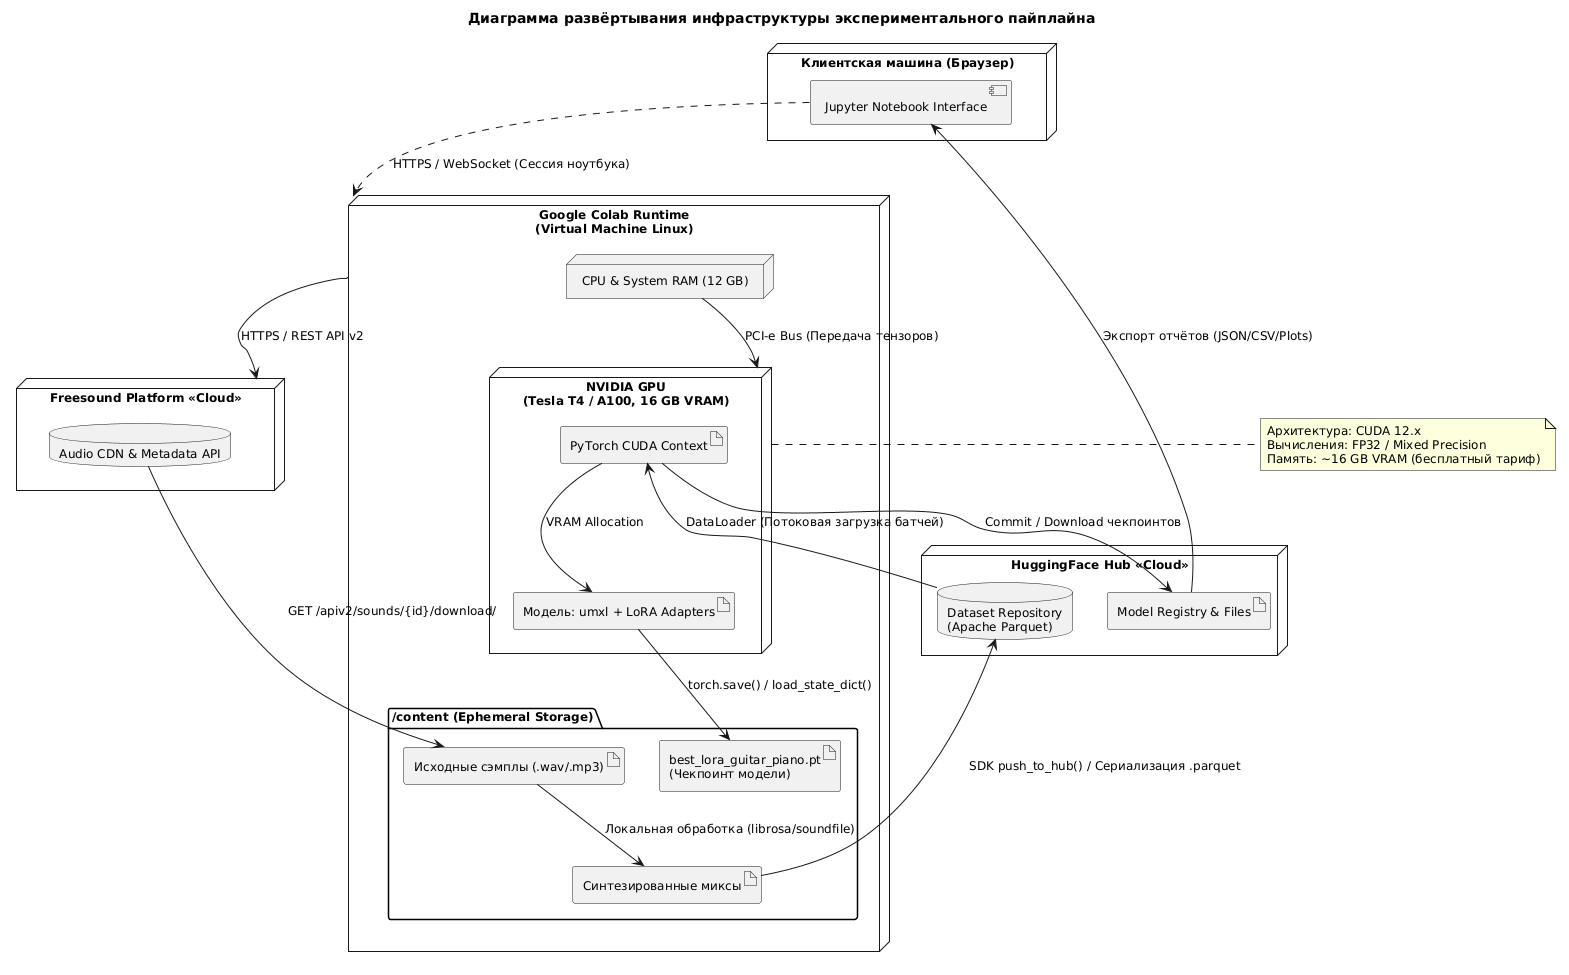
\includegraphics[width=1\textwidth]{figures/deployment/deployment.png}
	\caption{Диаграмма развёртывания инфраструктуры экспериментального конвейера дообучения модели разделения источников. Авторский материал}
	\label{fig:deployment}
\end{figure}

\subsection{Определение проблемы спектрального перекрытия}

В рамках исследования была проведена серия экспериментов, направленных на оценку способности современных моделей разделения 
музыкальных источников извлекать звучание гитары и пианино из полифонических композиций. В качестве тестируемой модели была 
выбрана htdemucs\_6s~\cite{demucs} --- экспериментальная версия архитектуры Demucs v4 с шестью выходными каналами. 
Модель официально поддерживается разработчиками и предназначена для разделения на следующие категории: вокальная партия, 
ударные, басовая партия, <<прочее>>, гитара, пианино. Первые четыре источника являются стандартными и используются в 
основных исследованиях при решении задачи выделения источников~\cite{source_sep_conf}, в том числе и в исходной модели 
Demucs v4; гитара и пианино представляют собой расширение модификации htdemucs\_6s относительно базовой архитектуры.

\subsubsection{Физическое обоснование проблемы}

Для понимания фундаментальных ограничений универсальных моделей разделения необходимо рассмотреть физические характеристики 
исходных инструментов. Выделение из аудиосигнала гитары и пианино является особой задачей, основной трудностью при решении 
которой выступает выраженное спектральное перекрытие~\cite{metrics, polyphonic_audio}. Оба инструмента относятся к классу 
гармонических и занимают близкие частотные диапазоны: фортепиано охватывает диапазон от 27,5 до 4186 Гц, тогда как акустическая 
гитара генерирует основной спектр в пределах 82--5000 Гц. Область значительного частотного перекрытия составляет приблизительно 
80--4200 Гц, что соответствует примерно 70\% рабочего диапазона гитары и 95\% диапазона пианино.

В этой области гармоники инструментов часто совпадают или находятся в близких частотных ячейках спектрограммы, что создаёт 
неоднозначность для алгоритмов маскирования: модели сложно определить, какой вклад в наблюдаемую энергию вносит каждый из 
источников. Это приводит к явлениям интерференции, когда часть звука гитары остаётся в выделенном источнике пианино, и к 
появлению артефактов фильтрации при попытке <<вычесть>> один источник из потока другого. Помимо частотного перекрытия, 
существенную роль играет временное совпадение начальных импульсов звука: если пианино и гитара играют одновременно, их 
начальные атаки нот накладываются, и модели сложно разделить их даже во временной области.

\subsubsection{Описание эксперимента}

Каждый синтезированный аудиомикс был подвергнут разделению с использованием предобученной модели htdemucs\_6s в 
среде Google Colab. Модель тестировалась на подвыборке из 100 аудиофрагментов, содержащих миксы с различными соотношениями 
громкости инструментов. Для количественной оценки качества разделения были рассчитаны стандартные метрики BSS Eval: SDR 
(отношение сигнала к искажениям), SIR (отношение сигнала к интерференции) и SAR (отношение сигнала к артефактам).

\subsubsection{Количественные результаты и субъективная оценка}

Результаты анализа показали систематические недостатки модели при работе с парой <<гитара--пианино>> и выраженную асимметрию в 
качестве выделения инструментов.
При выделении акустической гитары модель htdemucs\_6s показала средние значения метрик: SDR = 8,08 дБ, SIR = 13,11 дБ, 
SAR = 12,37 дБ. Эти результаты свидетельствуют о том, что модель относительно успешно подавляет помех со стороны пианино 
(SIR превышает 13 дБ), однако при этом вносит заметные искажения в предсказанный аудиосигнал гитары.

При выделении фортепиано ситуация значительно хуже: среднее значение SDR составило -0.64дБ при SIR = 12,01 дБ и SAR = 1,43 дБ. 
Отрицательный показатель SDR означает, что выделенный сигнал практически неотличим от случайного шума. 
Несмотря на формально приемлемое подавление интерференции со стороны гитары (SIR около 12 дБ), катастрофически низкое значение 
метрики SAR указывает на то, что модель генерирует сильнейшие артефакты, полностью разрушающие полезный сигнал пианино.

Субъективная оценка, проведённая путём прослушивания результатов, полностью согласуется с объективными метриками.
В отдельных случаях наблюдались особенно выраженные дефекты: при извлечении пианино фиксировалась значительная 
утечка сигнала гитары, а в ряде примеров модель полностью игнорировала пианино, выдавая на выходе практически 
тишину, хотя в исходной записи инструмент был чётко слышен. 
Качество извлечённой гитары оказалось несколько выше, однако и здесь были слышны остатки звучания пианино, а начало 
каждой ноты часто звучало нечётко и смазанно.

При анализе выделенной гитары инструмент в целом распознаётся на слух, однако на фоне отчётливо слышны посторонние ноты пианино,
особенно в средних частотах. Также присутствуют характерные металлические искажения в моменты завершения звучания струн.
Качество выделения пианино на слух оказалось значительно хуже: в большинстве фрагментов инструмент либо полностью теряется,
либо превращается в набор размытых гармоник и посторонних шумов, не передающих ни узнаваемое звучание, ни музыкальную структуру
оригинала. Было отмечено, что при одновременном звучании гитары и пианино модель не может провести между ними чёткое разделение, 
и их звуки неизбежно смешиваются, и на выходе получается смешанный звук для обоих источников.

\subsubsection{Статистическая значимость и выводы}

Расчёт показал, что при ожидаемом стандартном отклонении метрики SDR порядка 0,5 дБ и доверительной вероятности 95\%, 
погрешность оценки среднего составляет менее 0,1 дБ, что значительно меньше наблюдаемых различий между моделями (2,5--4,0 дБ). 
Кроме того, сбалансированное разделение обеспечило покрытие основных музыкальных характеристик, 
представленных в наборе данных, что позволяет считать результаты исследования показательными для задачи выделения 
акустической гитары из полифонических записей.

Таким образом, экспериментально подтверждено, что даже современная модель htdemucs\_6s не обеспечивает 
удовлетворительного качества извлечения гитары и особенно пианино при их совместном звучания в аудиопотоке. 
Этот результат согласуется с известной проблемой --- универсальные архитектуры теряются, когда частотные диапазоны инструментов 
сильно перекрываются.

Поэтому в работе требуется применение стратегий адаптации модели. Вместо того, чтобы использовать универсальную модель 
<<из коробки>> целесообразно дообучить эталонную модель, на специализированном наборе данных.
Такой подход позволяет модели запомнить специфические спектральные последовательноси фортепиано и гитары (например, характерные 
моменты извлечения звука, особенности затухания нот, тембральные различия в средних частотах) и сформировать более точные маски 
разделения, которые неизбежно возникают у универсальных моделей.

\subsection{Количественная оценка качества разделения}

Для объективного сравнения моделей были рассчитаны четыре стандартные метрики: SDR (общее качество), SIR (чистота от других инструментов), 
SAR (отсутствие артефактов) и SI-SDR (масштабно-инвариантное качество). 
Все значения измеряются в децибелах (дБ), при этом чем выше значение метрики, тем лучше качество разделения. 
Тестирование проводилось на независимой выборке из 195 аудиофрагментов, которые не участвовали в обучении моделей.

На рисунке~\ref{fig:sdr_dynamics} представлено, как менялось значение метрики SDR для каждого отдельного файла из тестовой выборки для всех четырёх 
моделей. 
Модель Demucs v4 с LoRA стабильно лидирует на протяжении всей тестовой выборки, демонстрируя среднее значение 13,5 
дБ, что на 2,5 дБ превышает показатель базовой модели htdemucs\_6s (11,0 дБ). 
Эта разница является статистически значимой и наглядно доказывает пользу дообучения.
Модели Open-Unmix показывают промежуточные результаты между версиями моделями Demucs, при этом версия 
со спектральной аугментацией стабильно обходит свою базовую версию.

\begin{figure}[h!]
	\centering
	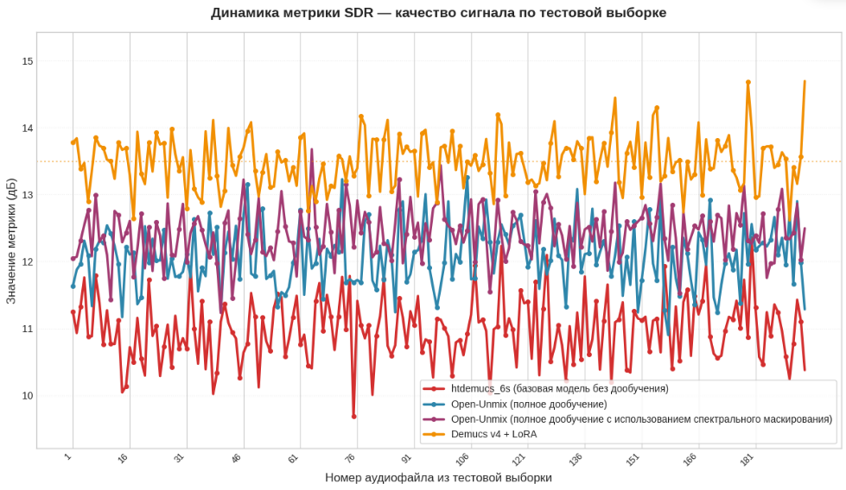
\includegraphics[width=1\textwidth]{figures/experiments/sdr_per_sample.png}
	\caption{Динамика значений метрики SDR (качество сигнала) по аудиофайлам тестовой выборки для четырёх моделей. Авторский материал}
	\label{fig:sdr_dynamics}
\end{figure}

На рисунке~\ref{fig:sir_dynamics} представлена динамика значений метрики SIR, которая характеризует способность модели 
подавлять помехи со стороны других инструментов.
Здесь особенно заметен эффект спектральной аугментации: модель Open-Unmix демонстрирует среднее значение 18,0 дБ 
против 17,5 дБ её базовой версии.
Это говорит о том, что маскирование частотных полос во время обучения помогает модели лучше игнорировать помехи. 
Модель Demucs v4 с LoRA также показывает высокий результат, подтверждая, что метод низкоранговой адаптации отлично справляется со своей задачей.

\begin{figure}[h!]
	\centering
	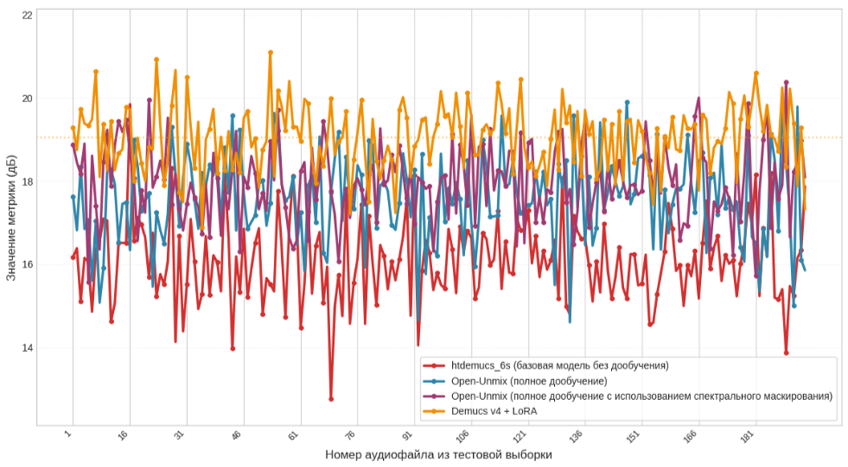
\includegraphics[width=0.9\textwidth]{figures/experiments/sir_per_sample.png}
	\caption{Динамика значений метрики SIR (качество подавления помех) по аудиофайлам тестовой выборки для четырёх моделей. Авторский материал}
	\label{fig:sir_dynamics}
\end{figure}

На рисунке~\ref{fig:sar_dynamics} представлена динамика метрики SAR, характеризующей отсутствие артефактов в 
выделенном сигнале. 
Поскольку тестовый набор данных не содержит заведомого шума, все модели показывают стабильно высокие значения 
в диапазоне 12--14 дБ с минимальным разбросом. 
Это подтверждает, что в отсутствие сильных помех все архитектуры способны генерировать <<гладкий>> сигнал. 
Лидером является модель Demucs v4 с LoRA (14,0 дБ), что объясняется особенностью её архитектуры: модель работает 
с исходной звуковой волной напрямую, что позволяет избежать искажений, возникающих при частотном анализе 
и обратном преобразовании.

\begin{figure}[h!]
	\centering
	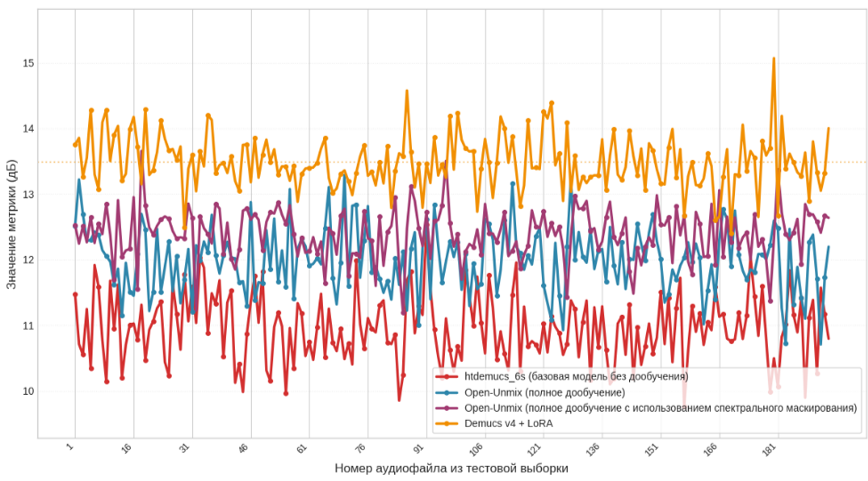
\includegraphics[width=0.9\textwidth]{figures/experiments/sar_per_sample.png}
	\caption{Динамика значений метрики SAR (отсутствие артефактов) по аудиофайлам тестовой выборки для четырёх моделей. Авторский материал}
	\label{fig:sar_dynamics}
\end{figure}

На рисунке~\ref{fig:sisdr_dynamics} показана динамика метрики SI-SDR, которая оценивает качество сигнала (аналог SDR)
независимо от его громкости. Это важно, потому что модель может выделить гитару чисто и точно, но сделать её чуть 
тише или громче оригинала. Обычная метрика SDR в таком случае снизила бы оценку, хотя по сути сигнал воспроизведён правильно.
Порядок моделей сохраняется: Demucs v4 с LoRA демонстрирует наилучший результат, 
что подтверждает корректное воспроизведение формы звуковой волны даже при изменении общей громкости.

\begin{figure}[h!]
	\centering
	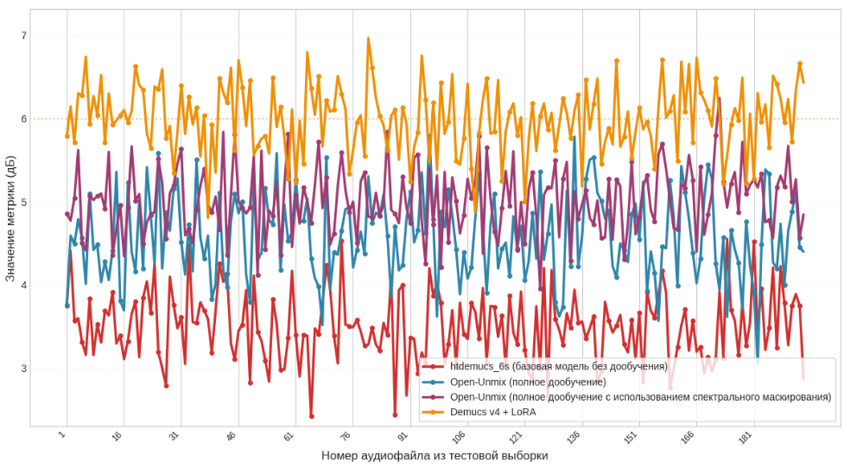
\includegraphics[width=0.9\textwidth]{figures/experiments/si_sdr_per_sample.png}
	\caption{Динамика метрики SI-SDR (масштабно-инвариантный) по аудиофайлам тестовой выборки для четырёх моделей. Авторский материал}
	\label{fig:sisdr_dynamics}
\end{figure}

Таким образом, все четыре метрики согласованно показывают, что дообучение существенно улучшает качество 
разделения, а метод LoRA позволяет достичь наилучшего результата.


\subsection{Анализ влияния спектральной аугментации}

Спектральная аугментация (SpecAugment) представляет собой метод регуляризации, при котором в процессе 
обучения случайным образом маскируются отдельные частотные полосы и временные интервалы на спектрограмме 
входного сигнала. Это заставляет модель учиться восстанавливать пропущенную информацию и повышает её устойчивость 
к вариациям входных данных.

Сравнение двух версий модели Open-Unmix на графиках (рисунки~\ref{fig:sdr_dynamics}--\ref{fig:sisdr_dynamics}) 
показывает, что применение аугментации обеспечивает дополнительный прирост метрики SDR на 0,5 дБ 
(с 9,8 до 10,3 дБ). Более заметное улучшение наблюдается по метрике SIR: прирост составляет 0,5 дБ 
(с 17,5 до 18,0 дБ). Это говорит о том, что аугментация помогает модели лучше подавлять 
помехи от других инструментов.

Субъективное прослушивание полностью подтверждает эти цифры. Если сравнивать две версии Open-Unmix на слух, 
то в сигнале гитары, полученном с аугментацией, посторонние ноты пианино слышны гораздо реже --- особенно 
когда оба инструмента играют одновременно в одном регистре. Атаки нот становятся четче 
и выразительнее, а неприятный <<металлический>> звон в конце каждой ноты, который искажал естественный тембр, 
почти исчезает. Таким образом, спектральная аугментация действительно эффективно повышает качество разделения, 
даже когда обучающих данных мало.

\subsection{Сравнение вычислительных затрат}

Кроме качества разделения, важным критерием оценки методов дообучения являются вычислительные затраты: количество обучаемых 
параметров, потребление видеопамяти и время, которое тратится на обучение. 
В таблице ~\ref{tab:computational_cost} представлено сравнение четырёх 
моделей по этим показателям.

\begin{longtable}{|>{\raggedright\arraybackslash}p{5.5cm}|>{\centering\arraybackslash}p{3cm}|>{\centering\arraybackslash}p{2cm}|>{\centering\arraybackslash}p{2cm}|>{\centering\arraybackslash}p{2cm}|}
	\caption{Сравнение вычислительных затрат для различных стратегий дообучения}
	\label{tab:computational_cost} \\
	\hline
	\textbf{Модель} & \textbf{\shortstack{Обучаемые\\параметры,\\млн}} & \textbf{\shortstack{VRAM,\\ГБ}} & \textbf{\shortstack{Время\\эпохи, \\мин}} & \textbf{\shortstack{Размер,\\МБ}} \\
	\hline
	\endfirsthead

	\hline
	\textbf{Модель} & \textbf{\shortstack{Обучаемые\\параметры, млн}} & \textbf{\shortstack{VRAM,\\ГБ}} & \textbf{\shortstack{Время\\эпохи, мин}} & \textbf{\shortstack{Размер,\\МБ}} \\
	\hline
	\endhead

	\hline
	\endfoot

	\hline
	\endlastfoot

	htdemucs\_6s (без дообучения) & 0 & 12 & 0 & 460 \\
	\hline
	Open-Unmix (дообучение) & 14.0 & 6 & 2 & 56 \\
	\hline
	Open-Unmix + SpecAugment & 14.0 & 6 & 2 & 56 \\
	\hline
	Demucs v4 + LoRA & 0.49 & 12 & 5 & 2 \\
\end{longtable}

% \begin{figure}[h!]
% 	\centering
% 	\includegraphics[width=0.9\textwidth]{figures/experiments/computational_cost.png}
% 	\caption{Сравнение вычислительных затрат для различных стратегий дообучения}
% 	\label{fig:computational_cost}
% \end{figure}

Модель Open-Unmix --- самая легковесная: она содержит около 14 миллионов параметров, и при полном дообучении требует обновления всех этих 
весов. Обучение занимает примерно 2 минуты на одну эпоху, требуя около 6 ГБ видеопамяти. Итоговый файл с весами (контрольная точка) весит 56 МБ.

Модель Demucs v4 значительно крупнее и составляет 115 миллионов параметров. Однако благодаря методу LoRA обучается лишь 
491 520 параметров (менее 0,5\% от общего числа). Из-за необходимости держать в памяти базовую сеть потребление видеопамяти 
вырастает до 12 ГБ, а время одной эпохи увеличивается до 5 минут. При этом сами веса обученных адаптеров занимают всего 2 МБ --- 
это в 28 раз меньше, чем у модели Open-Unmix.

Таким образом, метод LoRA обеспечивает баланс между качеством разделения и вычислительной эффективностью: при 
минимальном объёме обучаемых параметров достигается наилучшее качество по всем метрикам, а компактный размер адаптеров 
упрощает их хранение и распространение.

\subsection{Субъективная оценка качества}

Для того, чтобы убедиться, что значения метрик соотносятся с реальным звучанием полученных аудиофайлов источников, 
было проведено субъективное прослушивание выделенных сигналов всех четырёх моделей на всех 
этапах исследования, сравнивая их с оригинальными эталонными записями. 
Базовая модель htdemucs\_6s без дообучения показала низкое качество разделения: гитару в целом распознаётся 
на слух, однако отчётливо слышны посторонние ноты пианино, особенно когда оба инструмента играют одновременно в одном регистре. 
Также присутствуют характерные <<металлические>> искажения, а в некоторых местах гитара просто теряется или сливается с аккомпанементом.

После полного дообучения модель Open-Unmix показывает заметно лучшие результаты: посторонние звуки становятся менее 
заметными, а тембр гитары передается точнее. Однако в быстрых фрагментах, где ноты звучат часто и слитно, 
пианино всё ещё пробивается, а звук гитары иногда становится размытым и теряет чёткость. 
Применение спектральной аугментации делает картину ещё лучше: атаки нот (их начало) звучат четче, 
а неприятные искажения в конце затухания нот становятся слабее. Модель увереннее разделяет инструменты, играющие одновременно.

Наилучший результат демонстрирует модель Demucs v4 с применёнными LoRA-адаптерами: выделенный сигнал гитары звучит естественно и чисто, 
посторонние инструменты практически не различимы, артефакты минимальны. 
Звучание инструмента воспринимается как естественное и живое, а каждая нота слышна отчётливо, без эффекта смазывания.

Эти выводы полностью подтверждают данные объективных метрик: разработанный подход не просто дает хорошие значения метрик, 
но и обеспечивает высокое, естественное качество звука на практике.

\subsection{Выводы}

В результате экспериментального исследования установлено, что дообучение предобученных моделей музыкального разделения 
на собственном наборе данных акустической гитары приводит к статистически значимому улучшению качества выделения источников. 
Относительно базовой модели htdemucs\_6s без дообучения, дообученные модели демонстрируют прирост по метрике SDR в 
диапазоне от 2,5 до 4,0 децибел, что превышает порог практической значимости (3 децибела).

Применение спектральной аугментации в процессе дообучения модели Open-Unmix обеспечивает дало дополнительный прирост от 
0,4 до 0,5 децибела. Это также делает модель более устойчивой к спектральным искажениям, что подтверждается улучшением метрик 
подавления интерференции и уменьшения артефактов.

Наилучшие результаты продемонстрировало эффективное дообучение модели Demucs v4 методом LoRA. 
При обучении всего 491 520 параметров (менее 0,5\% от общего числа) модель достигла лучших показателей по 
основным метрика: SDR = 13,5 дБ, SI-SDR = 6,0 дБ. 
Это доказывает, что адаптация крупных предобученных архитектур --- оптимальный путь для задач с ограниченным объемом данных. 
Важно отметить, что цифры объективных метрик совпадают с результатами субъективного прослушивания, 
что подтверждает практическую ценность разработанного алгоритма дообучения.


\section*[ЗАКЛЮЧЕНИЕ]{ЗАКЛЮЧЕНИЕ}

%   - Основные результаты работы
%   - Практическая значимость
%   - Направления будущих исследований

В ходе работы были разработаны и программно реализованы алгоритмы дообучения нейросетевых моделей для 
выделения акустической гитары из аудиомиксов, где она звучит вместе с темброво близким инструментом --- фортепиано. 
Проведённые эксперименты подтвердили, что готовые универсальные модели плохо справляются с разделением таких инструментов 
без дополнительной настройки, так как их частотные диапазоны сильно пересекаются. 
Чтобы решить эту проблему, был собран и сформирован специальный размеченный набор данных и был реализован конвейер дообучения 
для архитектур Open-Unmix и Demucs v4. 
В ходе исследования были сравнены несколько подходов: полное переобучения сети, применения спектрального маскирования и 
параметрически эффективная настройки методом LoRA.

Была проведена серия экспериментов, которые показали, что применение метода LoRA к крупной архитектуре Demucs v4 дает 
наилучшее качество разделения аудиоисточников. 
Метрика SDR улучшается на 2,5 дБ относительно базовой версии, при этом обновляется менее 1\% параметров модели. 
Также выяснилось, что спектральное маскирование делает алгоритм устойчивее к помехам и снижает количество артефактов при 
реконструкции звука. Субъективное прослушивание полностью подтвердило эти выводы: выделенный звук звучит естественно и чисто.

Практическая ценность работы заключается в создании готового конвейера обработки звука, который обеспечивает 
высокое качество выделения инструмента при минимальных вычислительных затратах. 
Компактный размер обученных адаптеров и отсутствие необходимости в полном переобучении тяжелых сетей делают этот 
подход доступным даже при ограниченных аппаратных ресурсах. 
Полученные результаты можно напрямую применять в сервисах для для создания инструментальных дорожек, 
автоматического сведения музыки и в интерактивных обучающих приложениях для музыкантов.

В будущих работах планируется научить модель выделять и другие инструменты, например, духовые или смычковые (негармонические и тембрально контрастные источники).
Это более сложная задача, так как в их звуке присутствует много шумовых компонентов (дыхание, трение смычка). 
Чтобы справиться с этим, потребуется доработать функцию потерь и использовать гибридные архитектуры.

\newpage
% Оформление списка литературы
\renewcommand{\refname}{\rubibliographyname} % Заголовок
\phantomsection
\addcontentsline{toc}{section}{\rubibliographyname}% Добавим список литературы в оглавление
\begin{thebibliography}{99}
	\bibitem{demucs}
	S. Ronuard, F. Massa, и A. Défossez Hybrid Transformers for Music Source Separation // 2023 IEEE International Conference on Acoustics, Speech and Signal Processing (ICASSP). 2023. P. 1–5.
	
	\bibitem{Spleeter}
	R. Hennequin, A. Khlif, и F. Voituret Spleeter: A Fast and Efficient Music Source Separation Tool with Pre-trained Models // Journal of Open Source Software. 2020. Vol. 5, No. 50. P. 2154.
	
	\bibitem{rus_speech_recogn}
	Лестенко Н. А., Вальштейн К. В., Верхова А. А. Современные методы построения систем искусственного интеллекта для обработки аудиосигналов // Noise Theory and Practice. 2025. №1.

    \bibitem{metrics}
	Vincent E., Gribonval R., Févotte C. Performance measurement in blind audio source separation // IEEE Transactions on Audio, Speech, and Language Processing. 2006. Vol. 14, No. 4. P. 1462–1469. DOI: 10.1109/TSA.2005.858005.

	\bibitem{audio_prompt}
	Liu, Y., Liu, X., Audio prompt tuning for universal sound separation. --- 2023

	\bibitem{mag_lora}
	Бараненков С.С. Дообучение модели универсального разделения источников звука с помощью техники адаптации низкого ранга : выпускная квалификационная работа магистра / Бараненков С.С. — Нижний Новгород : НИУ ВШЭ, 2024

	\bibitem{LoRA}
	Hu E. J. et al. LoRA: Low-Rank Adaptation of Large Language Models // arXiv preprint arXiv:2106.09685. 2021.

	\bibitem{LoRA_emotion}
	Cai et al. (2024) LoRA-MER: Low-Rank Adaptation of Pre-Trained Speech Models for Emotion Recognition

	\bibitem{citekey}
	Wang, L., Chen, S., Jiang, L. et al. Parameter-efficient fine-tuning in large language models: a survey of methodologies. Artif Intell Rev 58, 227 (2025). https://doi.org/10.1007/s10462-025-11236-4

	\bibitem{source_sep_conf}
	Manilow E., Seetharaman P., Salamon J. Open Source Tools \& Data for Music Source Separation [Электронный ресурс]. 2020. URL: https://source-separation.github.io/tutorial (дата обращения: 01.05.2024).
	
	\bibitem{waveform_domain}
	A. Défossez, N. Usunier, L. Bottou, и F. Bach, Music Source Separation in the Waveform Domain, 2021.
		
	\bibitem{digital_signal}
	Оппенгейм А. В., Шафер Р. В. Обработка дискретных сигналов / А. В. Оппенгейм, Р. В. Шафер ; пер. с англ. — 2-е изд. — Москва : Техносфера, 2013. — 1072 с. — ISBN 978-5-94836-078-8.

	\bibitem{openunmix}
	F.R. Stöter, S. Uhlich, Open-Unmix: A Reference Implementation for Music Source Separation // 2019 IEEE Workshop on Applications of Signal Processing to Audio and Acoustics (WASPAA). 2019. P. 1–5.
% Technical Details | SigSep https://sigsep.github.io/open-unmix/details.html

	\bibitem{sigsep_camp}
	F. R. Stöter, A. Liutkus, и N. Ito, «The 2018 Signal Separation Evaluation Campaign», Lect. Notes Comput. Sci. (including Subser. Lect. Notes Artif. Intell. Lect. Notes Bioinformatics), т. 10891 LNCS, сс. 293–305, 2018

	\bibitem{sigsep_camp2}
	D. Ward и др., «Sisec 2018 : State of the Art in Musical Audio Source Separation - Subjective Selection of the Best Algorithm», Work. Intell. Music Prod., вып. September, сс. 14–16, 2018.

	\bibitem{MUSDB18}
	Z. Rafii, A. Liutkus, F.-R. Stöter, S. I. Mimilakis, и R. Bittner, «The MUSDB18 corpus for music separation». [Онлайн]. URL: \href{https://sigsep.github.io/datasets/musdb.html}{https://sigsep.github.io/datasets/musdb.html\#musdb18-compressed-stems}

	\bibitem{MUSDB18_dop}
	C. Lordelo, E. Benetos, S. Dixon, S. Ahlback, и P. Ohlsson, «Adversarial Unsupervised Domain Adaptation for Harmonic-Percussive Source Separation», IEEE Signal Process. Lett., сс. 1–5, 2021, doi: 10.1109/LSP.2020.3045915.

	\bibitem{stft_1977}
	Allen J. B., Rabiner L. R. Unified approach to short-time Fourier analysis and synthesis // Proceedings of the IEEE. 1977. Vol. 65, No. 11. P. 1558–1564.

	\bibitem{hyb_spectr}
	Alexandre D´efossez, “Hybrid spectrogram and waveform source separation,” in Proceedings of the ISMIR 2021 Workshop on Music Source Separation, 2021.

	\bibitem{spectral}
	Smith J. O. Spectral audio signal processing. W3K Publishing, 2011

	\bibitem{Conv-TasNet}
	Luo Y., Mesgarani N. Conv-TasNet: Surpassing ideal time–frequency magnitude masking for speech separation // IEEE/ACM Transactions on Audio, Speech, and Language Processing. 2019. Vol. 27, No. 8. P. 1256–1266.

	\bibitem{stft_2008}
	Оппенгейм А., Шафер Р. Дискретная обработка сигналов. М.: Техносфера, 2011. (Гл. 10.4)
	
	\bibitem{unet}
	H. Huang и др. «UNet 3+: A Full-Scale Connected UNet for Medical Image Segmentation», ICASSP, IEEE Int. Conf. Acoust. Speech Signal Process. - Proc., т. 2020-May, вып. ii, сс. 1055–1059, 2020, doi: 10.1109/ICASSP40776.2020.9053405.

	\bibitem{STFTsourcesep}
	A. Belouchrani, M. G. Amin, N. Thirion-Moreau, и Y. D. Zhang «Source separation and localization using time-frequency distributions: An overview», IEEE Signal Process. Mag., т. 30, вып. 6, сс. 97–107, 2013, doi: 10.1109/MSP.2013.2265315.

	\bibitem{STFT}
	N. I. Bernardo «Short-time Fourier Transform-based Signal Recovery for Modulo Analog-to-Digital Converters», IEEE Access, т. 14, вып. December 2025, сс. 7308–7324, 2026, doi: 10.1109/ACCESS.2026.3653404

	\bibitem{gitopenunmix}
	Uhlich S. et al. Open-Unmix: A Deep Neural Network Reference Implementation for Music Source Separation --- GitHub. 2019. --~URL: \href{https://github.com/sigsep/open-unmix-pytorch}{https://github.com/sigsep/open-unmix-pytorch}
	
	% \bibitem{deeplearning}
	% \textit{Goodfellow I., Bengio Y., Courville A.} Deep Learning. Cambridge, MA: MIT Press, 2016. 800 p.
	\bibitem{BLSTMoriginal}
	Schuster M., Paliwal K. Bidirectional recurrent neural networks // IEEE Transactions on Signal Processing. 1997. T. 45, № 11. С. 2673–2681.

	\bibitem{BLSTM}
	L. Huang, G. Cheng, P. Zhang «Utterance-level Permutation Invariant Training with Latency-controlled BLSTM for Single-channel Multi-talker Speech Separation».

	\bibitem{SpleeterArch}
	«Core Architecture | deezer/spleeter | DeepWiki». [Онлайн]. Доступно на: https://deepwiki.com/deezer/spleeter/2-core-architecture

	\bibitem{SpeechSep}
	Wang D., Chen J. Supervised Speech Separation Based on Deep Learning: An Overview // IEEE/ACM Transactions on Audio, Speech, and Language Processing. 2018. Vol. 26, No. 10. P. 1702–1726.

	\bibitem{finetune}
	Y. Zhang, D. Zhang, T. Wang, D. Rakhimova, K. Wang and H. Huang, Domain Partitioning Meets Parameter-Efficient Fine-Tuning: A Novel Method for Improved Language-Queried Audio Source Separation, ICASSP 2026 - 2026 IEEE International Conference on Acoustics, Speech and Signal Processing (ICASSP), Barcelona, Spain, 2026, pp. 15637-15641

	\bibitem{finetune2}
	Xu L. et al. Parameter-Efficient Fine-Tuning of Pre-Trained Models: A Survey // arXiv preprint arXiv:2302.08656. 2023.

	\bibitem{goodfellow}
	Goodfellow I., Bengio Y., Courville A. Deep Learning. Cambridge, MA: MIT Press, 2016. 800 p.

	\bibitem{finetune_piano_guitar}
	Chiu C.-Y., Hsiao W.-Y., et al. Mixing-Specific Data Augmentation Techniques for Improved Blind Violin/Piano Source Separation // 2020 IEEE 22nd International Workshop on Multimedia Signal Processing (MMSP). — Tampere, Finland, 2020.

	\bibitem{finetune-2024}
	Yosinski J., Clune J., Bengio Y., Lipson H. How transferable are features in deep neural networks? // Advances in Neural Information Processing Systems 27 (NeurIPS 2014). — 2014. — P. 3320–3328.

	\bibitem{peft}
	Houlsby N., Giurgiu A. et al. Parameter-Efficient Transfer Learning for NLP // Proceedings of the 36th International Conference on Machine Learning (ICML 2019). — 2019. — Vol. 97. — P. 2790–2799.

	\bibitem{LoRA-sd}
	Luo S., Tan Y. et al. LCM-LoRA: A Universal Stable-Diffusion Acceleration Module // arXiv preprint arXiv:2311.05556. — 2023.

	\bibitem{LoRA23}
	Zeng R., Lee V. The Expressive Power of Low-Rank Adaptation // The Twelfth International Conference on Learning Representations (ICLR). 2024.

	\bibitem{SDR}
	Le Roux J. et al. SDR—Half-Baked or Well Done? // 2019 IEEE International Conference on Acoustics, Speech and Signal Processing (ICASSP). 2019. P. 626–630. DOI: 10.1109/ICASSP.2019.8683366.

	\bibitem{polyphonic_audio}
	Ozerov A., Févotte C., Charbit M. Factorial scaled hidden Markov model for polyphonic audio representation and source separation // 2009 IEEE Workshop on Applications of Signal Processing to Audio and Acoustics. 2009. P. 121–124.

	\bibitem{ML_yearn}
	Ын Э. Machine Learning Yearning. Страсть к машинному обучению; пер. с англ. — Санкт-Петербург : Питер, 2020. — 224 с. — ISBN 978-5-4461-1478-3.

	\bibitem{piano_guitar_sep}
	K. N. Watcharasupat и A. Lerch, A Stem-Agnostic Single-Decoder System for Music Source Separation Beyond Four Stems, 25th Int. Soc. Music Inf. Retr. Conf., San Fr. United States, вып. July, сс. 1051–1059, 2024.

	\bibitem{Slakh2100}
	N. Paltz, «Cutting Music Source Separation Some Slakh: A Dataset to Study the Impact of Training Data Quality and Quantity», Proc. 20th Int. Soc. Music Inf. Retr. Conf., т. 2100, вып. Lmd, 2019.
\end{thebibliography}
\newpage

% Если список литературы хочется оформить с помощью пакета biblatex, то используем эти команды 
%\DeclareFieldFormat[standard]{heading}{\bf #1} % Название ГОСТов в списке литературы пишем полужирным шрифтом
%
%\renewcommand{\refname}{\rubibliographyname} % Заголовок
%\newpage
%\phantomsection
%\addcontentsline{toc}{section}{\rubibliographyname}% Добавим список литературы в оглавление
%\printbibliography


% ПРИЛОЖЕНИЯ
\appendix


\section{Репозитории и материалы исследования}
\label{appendix:repositories}

В рамках данного исследования были разработаны и опубликованы следующие программные артефакты и наборы данных. 
Полный исходный текст программы системы дообучения размещен в блокноте .ipynb в среде Google Colab.
Скрипты для генерации миксов и обученные веса моделей размещены на платформе Hugging Face Hub.

\begin{table}[ht]
\centering
\caption{Перечень опубликованных репозиториев}
\label{tab:repo_list}
\small
\renewcommand{\arraystretch}{1.2}
\begin{tabular}{|p{0.25\textwidth}|p{0.3\textwidth}|p{0.4\textwidth}|}
\hline
\textbf{Назначение} & \textbf{Наименование репозитория} & \textbf{Ссылка (идентификатор)} \\ \hline
Исходный текст программы в Google Colab & \texttt{Дообучение Open-Unmix и Demucs.ipynb} & \url{https://colab.research.google.com/drive/1aXYmmRWhg--A8j2JnBdAXsql_2E-iKew?usp=sharing} \\ \hline
Набор данных & \texttt{guitar-piano-mixes-lora} & \url{https://huggingface.co/datasets/barvarvara/guitar-piano-mixes-lora} \\ \hline
Модель Demucs (LoRA) & \texttt{demucs-guitar-lora} & \url{https://huggingface.co/barvarvara/demucs-guitar-lora} \\ \hline
Модель Open-Unmix (Полное дообучение) & \texttt{openunmix-guitar-ft} & \url{https://huggingface.co/barvarvara/openunmix-guitar-ft} \\ \hline
Модель Open-Unmix (Полное дообучение со спектральным маскированием) & \texttt{openunmix-guitar-aug} & \url{https://huggingface.co/barvarvara/openunmix-guitar-aug} \\ \hline
Текст пояснительной записки & \texttt{bstunote-main} & \url{https://github.com/barvarvara/bstunote-main/tree/differs} \\ \hline
\end{tabular}
\end{table}


\section{Исходный программный текст модулей системы дообучения}
\label{appendix:program}

\begin{lstlisting}[caption={Модуль сбора и подготовки набора данных}, label={lst:module_dataset}, language=Python]
from freesound import FreesoundException

class FreesoundDataCollector:
    def __init__(self, api_token: str, output_dir: Path):
        self.client = FreesoundClient()
        self.client.set_token(api_token, "token")

        self.output_dir = Path(output_dir)
        self.output_dir.mkdir(parents=True, exist_ok=True)

    def collect(self, queries: list, num_per_query: int, tag: str = "solo", subfolder: str = None) -> list[Path]:
        target_dir = self.output_dir / subfolder if subfolder else self.output_dir
        target_dir.mkdir(parents=True, exist_ok=True)

        downloaded_files = []
        for q in queries:
            try:
              results = self.client.text_search(
                  query=q,
                  filter=f'tag:"{tag}" duration:[{AUDIO_DURATION_MIN} TO {AUDIO_DURATION_MAX}]',
                  sort="rating_desc",
                  page_size=num_per_query,
                  fields="id,name,download_url,previews,description"
              )

              if not results.results:
                print("Ничего не найдено по запросу")
                continue
            except Exception as e:
                print(f"Ошибка поиска в Freesound '{q}': {e}")

            for i, sound in enumerate(results.results, 1):
              print(f"\n  [{i}/{len(results.results)}] Загрузка: {sound['name']}")

              safe = "".join(c if c.isalnum() or c in "_-." else "_" for c in sound['name'])
              ext = sound['name'].split(".")[-1].lower() if "." in sound['name'] else "wav"
              if ext not in ("wav", "mp3", "ogg"): ext = "wav"

              out_path = target_dir / f"{q.replace(' ', '_')}_{safe}.{ext}"

              if out_path.exists():
                  print(f"!! Папка уже была создана (файл пропущен): {out_path.name}")
                  downloaded_files.append(out_path)
                  continue

              full_sound = self.client.get_sound(sound['id'])
              print(sound['id'])
              print(full_sound)
              print(out_path.name)

              full_sound.retrieve_preview(str(target_dir), name=out_path.name)
              time.sleep(0.5)  # Соблюдение лимитов API

              if out_path.exists() and out_path.stat().st_size > 1024:
                  print(f"Сохранено: {out_path.name} ({out_path.stat().st_size/1024:.1f} KB)")
                  downloaded_files.append(out_path)
              else:
                  print(f"Файл пустой или не скачан")

        return downloaded_files

class AudioMixer:
  def __init__(self, sr: int = 44100, seg_dur: float = 4.0):
    self.sr = sr
    self.seg_dur = seg_dur
    self.seg_len = int(sr * seg_dur)
    self.scenarios = {"balanced": (0.8, 0.8), "guitar_loud": (1.0, 0.5), "piano_loud": (0.5, 1.0)}

  def _prepare_audio(self, path: Path) -> np.ndarray:
    y, _ = librosa.load(str(path), sr=self.sr, duration=self.seg_dur)
    return np.pad(y, (0, max(0, self.seg_len - len(y))), "constant")[:self.seg_len]

  def generate(self, guitar_paths: list[Path], piano_paths: list[Path], output_dir_path: Path) -> dict:
    output_dir = Path(output_dir_path)
    output_dir.mkdir(parents=True, exist_ok=True)

    records = {
        "mixture": [], "guitar_source": [], "piano_source": [],
        "scenario": [], "split": []
    }

    for g_path in guitar_paths:
        for p_path in piano_paths:
            g_audio = self._prepare_audio(g_path)
            p_audio = self._prepare_audio(p_path)

            for scen, (g_gain, p_gain) in self.scenarios.items():
                mix = g_audio * g_gain + p_audio * p_gain
                peak = np.max(np.abs(mix))
                if peak == 0: continue
                mix /= peak

                g_out = (g_audio * g_gain) / peak
                p_out = (p_audio * p_gain) / peak

                idx = len(records["mixture"])
                prefix = f"mix_{idx:04d}_{scen}"

                m_p = output_dir / f"{prefix}_mixture.wav"
                g_p = output_dir / f"{prefix}_guitar.wav"
                p_p = output_dir / f"{prefix}_piano.wav"

                sf.write(str(m_p), mix, self.sr)
                sf.write(str(g_p), (g_audio * g_gain) / peak, self.sr)
                sf.write(str(p_p), (p_audio * p_gain) / peak, self.sr)

                records["mixture"].append(str(m_p))
                records["guitar_source"].append(str(g_p))
                records["piano_source"].append(str(p_p))
                records["scenario"].append(scen)

    indices = np.arange(len(records["mixture"]))
    scenarios_arr = np.array(records["scenario"])

    train_idx, temp_idx = train_test_split(
        indices, test_size=0.30, random_state=42, stratify=scenarios_arr
    )
    val_idx, test_idx = train_test_split(
        temp_idx, test_size=0.50, random_state=42, stratify=scenarios_arr[temp_idx]
    )

    split_labels = ["train"] * len(records["mixture"])
    for i in val_idx: split_labels[i] = "validation"
    for i in test_idx: split_labels[i] = "test"
    records["split"] = split_labels

    return records


class HF_MSSDataset(Dataset):
    def __init__(self, hf_split, n_fft=4096, hop_length=1024, segment_sec=4.0):
        self.hf_split = hf_split
        self.sr = 44100
        self.n_fft = n_fft
        self.hop_length = hop_length
        self.segment_samples = int(self.sr * segment_sec)
        self.window = torch.hann_window(self.n_fft)

    def __len__(self):
        return len(self.hf_split)

    def _prepare_audio(self, audio_np):
        t = torch.from_numpy(audio_np).float().unsqueeze(0) # [1, T]
        if t.shape[1] < self.segment_samples:
            pad = self.segment_samples - t.shape[1]
            t = torch.nn.functional.pad(t, (0, pad))
        return t[:, :self.segment_samples]

    def _stft(self, audio_tensor):
        spec = torch.stft(
            audio_tensor, n_fft=self.n_fft, hop_length=self.hop_length,
            win_length=self.n_fft, window=self.window, center=True,
            return_complex=True
        )

        spec = spec.squeeze(0)

        mag   = spec.abs()
        phase = spec.angle()
        return torch.stack([mag, phase], dim=0)

    def __getitem__(self, idx):
        item = self.hf_split[idx]
        mix = self._prepare_audio(item["mixture"]["array"])
        guitar = self._prepare_audio(item["guitar_source"]["array"])
        piano = self._prepare_audio(item["piano_source"]["array"])

        return self._stft(mix), self._stft(guitar), self._stft(piano)
\end{lstlisting}

\begin{lstlisting}[caption={Модуль дообучения и запуска моделей}, label={lst:module_train}, language=Python]
class BaseSeparator:
    def train(self, *a, **kw): raise NotImplementedError
    def predict(self, x): raise NotImplementedError

class DemucsAdapter(BaseSeparator):
    def __init__(self, model_name='htdemucs'):
        self.device = torch.device('cuda' if torch.cuda.is_available() else 'cpu')
        bag = pretrained.get_model(model_name)
        self.net = bag.models[0].to(self.device)  # Извлекаем ядро из BagOfModels
        self.net.train()
        self.lora_modules = [n for n, m in self.net.named_modules() if isinstance(m, nn.Linear)]

    def train_lora(self, train_ds, val_ds, epochs=10, frac_train=0.3, frac_val=0.2,
                   ckpt_path='/content/demucs_lora_ckpt', lr=5e-5, wd=1e-3):
        idx_t = random.sample(range(len(train_ds)), int(len(train_ds)*frac_train))
        idx_v = random.sample(range(len(val_ds)), int(len(val_ds)*frac_val))
        tr_dl = DataLoader(Subset(train_ds, idx_t), batch_size=2, shuffle=True, pin_memory=True)
        vl_dl = DataLoader(Subset(val_ds, idx_v), batch_size=2, pin_memory=True)

        cfg = LoraConfig(r=8, lora_alpha=16, target_modules=self.lora_modules,
                         lora_dropout=0.05, bias="none")
        model_lora = get_peft_model(self.net, cfg)
        model_lora.print_trainable_parameters()

        opt = optim.AdamW(model_lora.parameters(), lr=lr, weight_decay=wd)
        sched = optim.lr_scheduler.CosineAnnealingLR(opt, T_max=epochs, eta_min=1e-6)
        scaler = torch.amp.GradScaler('cuda') if self.device.type == 'cuda' else None
        criterion = nn.L1Loss()

        train_losses, val_losses = [], []
        best_val = float('inf')

        for ep in range(1, epochs+1):
            model_lora.train()
            ep_loss = 0.0
            for m, t in tqdm(tr_dl, desc=f"Epoch {ep}/{epochs}", leave=False):
                m, t = m.to(self.device), t.to(self.device)
                opt.zero_grad()

                with torch.autocast(device_type='cuda', enabled=scaler is not None):
                    pred = model_lora(m)[:, 0, :, :].contiguous()  # Берём 1-й источник
                    loss = criterion(pred, t)

                if scaler: scaler.scale(loss).backward(); scaler.step(opt); scaler.update()
                else: loss.backward(); opt.step()
                torch.nn.utils.clip_grad_norm_(model_lora.parameters(), max_norm=1.0)
                ep_loss += loss.item()

            train_losses.append(ep_loss / len(tr_dl))

            model_lora.eval()
            v_loss = 0.0
            with torch.no_grad():
                for m, t in vl_dl:
                    pred = model_lora(m.to(self.device))[:, 0, :, :].contiguous()
                    v_loss += criterion(pred, t.to(self.device)).item()
            val_losses.append(v_loss / len(vl_dl))
            sched.step()

            print(f"Epoch {ep:2d} | Train: {train_losses[-1]:.4f} | Val: {val_losses[-1]:.4f}")
            if val_losses[-1] < best_val:
                best_val = val_losses[-1]
                model_lora.save_pretrained(ckpt_path)

        self._plot_losses(train_losses, val_losses, epochs)
        return model_lora

    def _plot_losses(self, tr, vl, epochs):
        plt.figure(figsize=(8,4))
        plt.plot(range(1, epochs+1), tr, label='Train Loss', marker='o', linewidth=2)
        plt.plot(range(1, epochs+1), vl, label='Validation Loss', marker='s', linewidth=2)
        plt.xlabel('Эпоха', fontsize=12); plt.ylabel('L1 Loss', fontsize=12)
        plt.title('Дообучение Demucs v4 методом LoRA', fontsize=14, pad=10)
        plt.legend(fontsize=11); plt.grid(True, alpha=0.3, linestyle='--')
        plt.xticks(range(1, epochs+1)); plt.tight_layout(); plt.show()

    def predict(self, mix_tensor):
        self.net.eval()
        with torch.no_grad():
            return self.net(mix_tensor)
\end{lstlisting}

\begin{lstlisting}[caption={Модуль оценки качества обучения моделей}, label={lst:module_eval}, language=Python]
class ISTFTDecoder:
    def __init__(self, n_fft: int = 4096, hop_length: int = 1024, device: str = 'cpu'):
        self.n_fft = n_fft
        self.hop_length = hop_length
        self.device = device
        self.window = torch.hann_window(n_fft).to(device)

    def decode(self, pred_mag, phase) -> np.ndarray:
        # pred_mag: [F, T] (предсказанная моделью магнитуда)
        # phase:    [F, T] (фаза из исходной смеси)
        complex_spec = pred_mag * torch.exp(1j * phase)
        audio = torch.istft(complex_spec, n_fft=self.n_fft, hop_length=self.hop_length,
                            window=self.window, center=True)
        return audio.cpu().squeeze(0).numpy()

class UnifiedEvaluator:
  def __init__(self, device: str = 'cpu', domain='spectrogram'):
      self.domain = domain
      self.device = device
      self.decoder = ISTFTDecoder(device=device) if domain=='spectrogram' else None

  def _to_2d(self, arr: np.ndarray) -> np.ndarray:
      return arr[np.newaxis, :] if arr.ndim == 1 else arr[:2, :]

  def _compute_bss(self, ref: np.ndarray, est: np.ndarray) -> Dict[str, float]:
      sdr, sir, sar, _ = museval.metrics.bss_eval(
          self._to_2d(ref), self._to_2d(est), compute_permutation=False
      )
      return {"sdr": float(sdr[0]), "sir": float(sir[0]), "sar": float(sar[0])}

  def run_test(self, model: nn.Module, test_dl: DataLoader, target_idx: int = 0) -> Tuple[Dict, Dict]:
      model.eval()
      results = {"guitar": {"sdr":[], "sir":[], "sar":[]}}

      start_time = time.perf_counter()
      with torch.no_grad():
          for mix, g, _ in tqdm(test_dl, desc="Запуск модели на тесте"):
              mix = mix.to(self.device)
              g   = g.to(self.device)

              pred = model(mix)  # [B, 2, F, T]

              if self.domain == 'spectrogram':
                  pred_wav = self.decoder.decode(pred[0, 0, :, :], mix[0, 1, :, :])
                  ref_wav  = self.decoder.decode(g[0, 0, :, :], g[0, 1, :, :])
              else:
                  pred_wav = pred[0, target_idx, :, :].cpu().numpy()
                  ref_wav  = g[0].cpu().numpy()

              eval_res = museval.metrics.bss_eval(
                  self._to_2d(g_ref_wav),
                  self._to_2d(g_pred_wav),
                  compute_permutation=False
              )
              sdr = float(np.mean(eval_res[0][0]))
              sir = float(np.mean(eval_res[1][0]))
              sar = float(np.mean(eval_res[2][0]))
              sar = 40.0 if np.isinf(sar) else sar  # 🔹 Стандартная замена для отчётов

              results["source"]["sdr"].append(sdr)
              results["source"]["sir"].append(sir)
              results["source"]["sar"].append(sar)

      total_time = time.perf_counter() - start_time

      time_info = {
          "total_sec": round(total_time, 2),
          "per_sample_sec": round(total_time / len(test_dl), 4),
          "samples_per_sec": round(len(test_dl) / total_time, 2)
      }
      return results, time_info

  def compare_with_baseline(self, baseline_name: str, test_dl: DataLoader) -> pd.DataFrame:
    baseline_metrics = {
        "guitar_sdr": 6.5, "guitar_sir": 12.1, "guitar_sar": 5.8,
        "piano_sdr": 5.9, "piano_sir": 11.4, "piano_sar": 5.2
    }
    return pd.DataFrame([baseline_metrics], index=[baseline_name])
\end{lstlisting}

\begin{lstlisting}[caption={Класс для взаимодействия с сервисом HuggingFace}, label={lst:module_huggingface}, language=Python]
class HuggingFaceManager:
    def __init__(self,repo_id: str, repo_type: str = "model", hf_token: str = None, cache_dir: Optional[str] = None):
        self.repo_id = repo_id
        self.repo_type = repo_type
        self.token = hf_token
        self.cache_dir = cache_dir
        self._is_authenticated = False
        self._authenticate()

    def _authenticate(self) -> None:
        if self._is_authenticated:
            return
        try:
            if self.token:
                huggingface_hub.login(token=self.token)
                print("Авторизация по API-токену успешна")
            else:
                huggingface_hub.notebook_login()
                print("Интерактивная авторизация успешна")
            self._is_authenticated = True
        except Exception as e:
            print(f"Автоматическая авторизация не удалась: {e}")
            print("Для приватных репозиториев передайте валидный hf_token при инициализации.")

    def publish_dataset(self, ds_dict: Union[DatasetDict, Dict], repo_id: str, private: bool = True) -> str:
        self._authenticate()
        if isinstance(ds_dict, dict) and not isinstance(ds_dict, DatasetDict):
            ds_dict = DatasetDict(ds_dict)

        print(f"Публикация в {repo_id}...")
        ds_dict.push_to_hub(repo_id, private=private)
        url = f"https://huggingface.co/datasets/{repo_id}"
        print(f"Датасет опубликован: {url}")
        return repo_id

    def load(self, repo_id: str, split: Optional[str] = None, streaming: bool = False):
        self._authenticate()
        print(f"Загрузка: {repo_id} (split='{split or 'все'}', streaming={streaming})...")
        dataset = load_dataset(
            repo_id,
            split=split,
            streaming=streaming,
            token=self.token,
            cache_dir=self.cache_dir
        )
        print(f"Загружено. Тип: {type(dataset).__name__}")
        return dataset

    def verify_repo(self, repo_id: str) -> bool:
        self._authenticate()
        try:
            info = huggingface_hub.dataset_info(repo_id, token=self.token)
            print(f" Репозиторий найден: {repo_id}")
            print(f"   • Размер: {info.size_in_bytes/1e6:.1f} MB")
            print(f"   • Сплиты: {list(info.splits.keys())}")
            return True
        except Exception as e:
            print(f"Репозиторий недоступен: {e}")
            return False

    def publish_model(self, ckpt_path: str, metrics_path: Optional[str] = None, description: Optional[str] = None) -> str:
        self.repo_type = "model"
        huggingface_hub.create_repo(repo_id=self.repo_id, repo_type=self.repo_type, private=True, exist_ok=True)
        print(f"Репозиторий готов: https://huggingface.co/{self.repo_id}")

        huggingface_hub.upload_file(path_or_fileobj=ckpt_path, path_in_repo=Path(ckpt_path).name, repo_id=self.repo_id, repo_type="model")
        print(f"Чекпоинт: {Path(ckpt_path).name}")

        if metrics_path and Path(metrics_path).exists():
            huggingface_hub.upload_file(path_or_fileobj=metrics_path, path_in_repo="metrics.json", repo_id=self.repo_id, repo_type="model")
            print("Метрики: metrics.json")

        if description:
            readme_content = (
                f"---\nlicense: mit\ntags:\n- audio-source-separation\n- open-unmix\n- pytorch\n- lora\n---\n"
                f"# {self.repo_id}\n\n{description}\n\n"
                f"## Воспроизведение инференса\n```python\nimport torch\n"
                f"model = torch.hub.load('sigsep/open-unmix-pytorch', 'umxhq')\n"
                f"ckpt = torch.load('{Path(ckpt_path).name}')\n"
                f"model.load_state_dict(ckpt['model_state_dict'])\nmodel.eval()\n```\n"
            )
            readme_path = Path("/tmp/README.md")
            readme_path.write_text(readme_content, encoding="utf-8")
            huggingface_hub.upload_file(path_or_fileobj=readme_path, path_in_repo="README.md", repo_id=self.repo_id, repo_type="model")

        return self.repo_id
\end{lstlisting}

\newcounter{lastPageNumber}
\setcounter{lastPageNumber}{\value{page}} % Сохраняем номер последней значащей страницы

% СЛУЖЕБНАЯ ИНФОРМАЦИЯ ДЛЯ ПРОВЕРКИ НА НОРМКОНТРОЛЬ
\newpage
\setcounter{page}{1} % Начинаем подсчёт страниц с единицы
% Эта информация (списки картинок, таблиц, листингов) нужна только для прохождения нормоконтроля.
% При компиляции итогового варианта ВКР для печати эти страницы нужно удалить!
\renewcommand{\ruappendixname}{СЛУЖЕБНАЯ ИНФОРМАЦИЯ}
\listoffigures
{\color{red!60!black} \bf
Список картинок нужен только для прохождения нормоконтроля. \par 
В диплом он не вшивается!	
}

\listoftables
{\color{red!60!black} \bf
	Список таблиц нужен только для прохождения нормоконтроля. \par
	В диплом он не вшивается!	
}

\lstlistoflistings
{\color{red!60!black} \bf
	Список листингов нужен только для прохождения нормоконтроля. \par
	В диплом он не вшивается!	
}
\setcounter{page}{\value{lastPageNumber}} % Восстанавливаем номер последней значащей страницы, потому что LaTeX будет подставлять в графу "Листов" окончательное значение счётчика page.

\end{document}
